\documentclass[titlepage]{article}

\usepackage[letterpaper,margin=1in,footskip=0.25in]{geometry}
\usepackage[hidelinks]{hyperref}
\usepackage{fancyhdr}
\usepackage{csquotes}
\usepackage{amsmath}
\usepackage{tikz}
\usepackage{subcaption}
\usepackage{graphicx}
\usepackage{amssymb}
\usepackage{float}
\usepackage{amssymb}

\MakeOuterQuote{"}

\numberwithin{figure}{section}
\numberwithin{table}{section}
\numberwithin{equation}{section}

\usetikzlibrary{knots,decorations.markings}

\newcommand{\dq}[2]{``#1" (#2).}

\renewcommand{\labelitemiii}{\scriptsize$\blacksquare$}

\title{{\Huge\emph{The Knot Book}}\\[5pt]\textcolor{gray!60!black}{Notes}\vspace{-0.5em}}
\author{Steven Labalme}
\date{\today}

\begin{document}




\pagenumbering{gobble}
\maketitle



\pagenumbering{roman}
\tableofcontents
\listoffigures
\listoftables
\newpage



\pagenumbering{arabic}
\pagestyle{fancy}
\fancyhf{}
\rfoot{Labalme \thepage}
\renewcommand{\headrulewidth}{0pt}
\section{Introduction}\label{sse:intro}
\subsection{Introduction}\label{sss:Introduction}
\begin{itemize}
    \item \textbf{Knot}: \dq{A knotted loop of string, except that we think of the string as having no thickness, its cross-section being a single point}{2}
    \item Do not distinguish between a `nice, even' knot and one that has been deformed through space.
    \item \textbf{Unknot}: \dq{The simplest knot of all\dots the unknoted circle}{2} \emph{Also known as} \textbf{trivial knot}. See Figure \ref{fig:circletrefoila}.
    \item \textbf{Trefoil knot}: \dq{The next simplest knot}{2} See Figure \ref{fig:circletrefoilb}.
    \begin{figure}[h!]
        \centering
        \begin{subfigure}{0.2\linewidth}
            \centering
            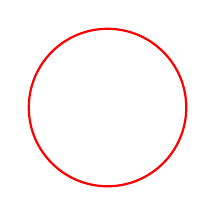
\begin{tikzpicture}
                \draw[red,thick] (0,0) circle (1cm);
            \end{tikzpicture}
            \caption{Trivial knot.}
            \label{fig:circletrefoila}
        \end{subfigure}
        \begin{subfigure}{0.2\linewidth}
            \centering
            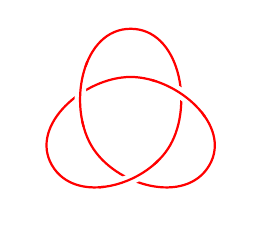
\begin{tikzpicture}
                \begin{knot}[
                    consider self intersections,
                    clip width=5
                ]
                    % could be defined with a combination of polar coordinates and foreach...
                    \strand[red,thick] (1,{3^0.5})
                        to [out=0,in=60] (1.5,0.25)
                        to [out=240,in=-60] (0,0)
                        to [out=120,in=180] (1,1.12)
                        to [out=0,in=60] (2,0)
                        to [out=240,in=-60] (0.5,0.25)
                        to [out=120,in=180] cycle
                    ;
                    \flipcrossings{1,3}
                \end{knot}
            \end{tikzpicture}
            \caption{Trefoil knot.}
            \label{fig:circletrefoilb}
        \end{subfigure}
        \caption{Projections of the two simplest knots.}
        \label{fig:circletrefoil}
    \end{figure}
    \item \textbf{Projection}: A picture of a knot, such as those in Figure \ref{fig:circletrefoil}.
    \begin{itemize}
        \item The same knots can have multiple projections (as they are deformed in space).
    \end{itemize}
    \item \textbf{Crossings}: The places in a projection where a knot crosses itself.
    \begin{itemize}
        \item The trefoil knot in Figure \ref{fig:circletrefoilb} is a \underline{three-crossing knot} because it crosses itself 3 times.
        \item Any one-crossing knot is trivial.
        \item \emph{Exercise 1.2}: Any two-crossing knot must be trivial because the simplest nontrivial knot is the trefoil knot, which has three crossings.
    \end{itemize}
    \item Atoms were originally thought to be tangles (knots) in the ether of the universe, but when chemists moved on, mathematicians took up knot theory. In the 1980s, biochemists began to see applications of knot theory in their research (see Section \ref{sse:biochemphys}).
    \item \textbf{Topology}: \dq{The study of the properties of geometric objects that are preserved under deformations}{6}
    \begin{itemize}
        \item Knot theory is a subfield of topology (see Section \ref{sse:topology}).
    \end{itemize}
    \begin{figure}[h!]
        \centering
        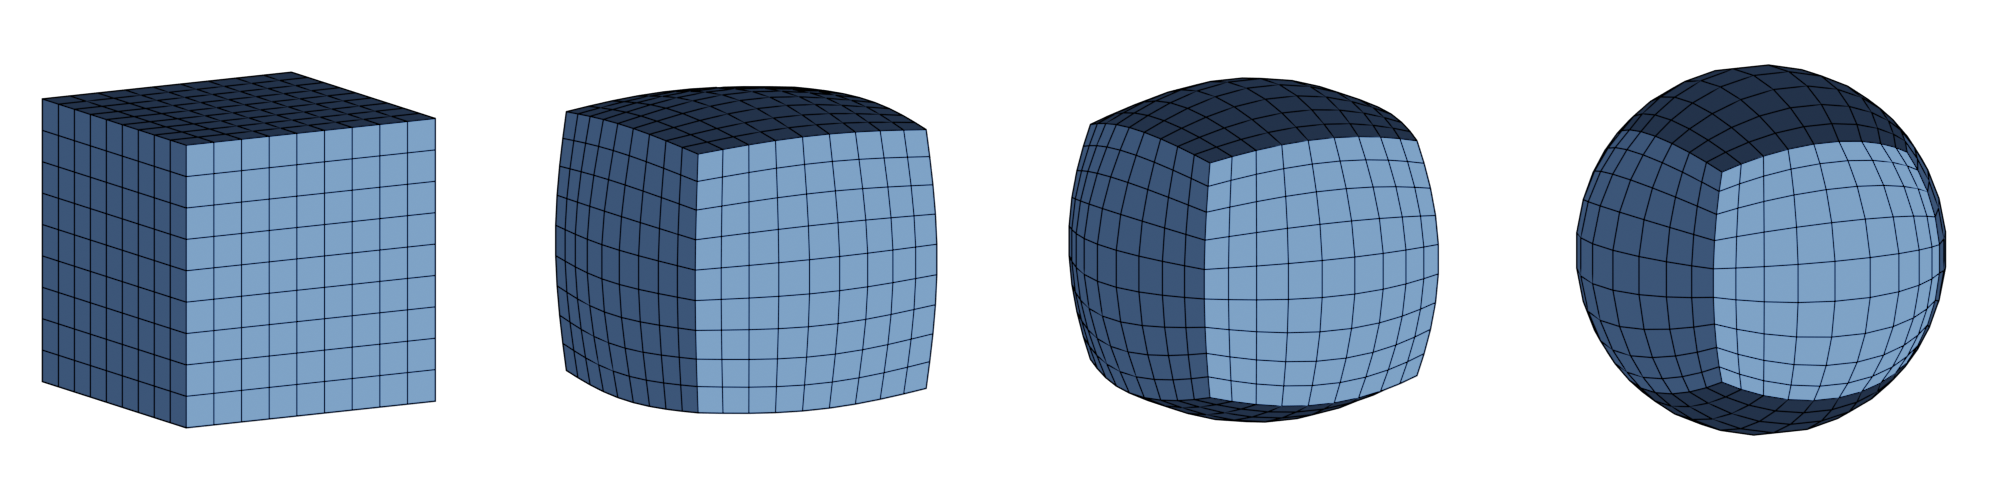
\includegraphics[width=0.7\linewidth]{Blender/CubeSphere.png}
        \caption{Deformation of a cube into a sphere.}
        \label{fig:cubesphere}
    \end{figure}
    \item Any knot can have a projection with as many crossings as desired.
    \item \textbf{Alternating knot}: \dq{A knot with a projection that has crossings that alternate between over and under as one travels around the knot in a fixed direction}{7}
    \begin{itemize}
        \item The trefoil is such a knot.
    \end{itemize}
    \item \emph{Exercise 1.7*}: By changing some of the crossings from over to under or vice versa, any projection of a knot can be made into a projection of the unknot$^[$\footnote{How can I \emph{show} something? How can I do these proofs? What kind of logic solves one of these? See Section \ref{sss:UnknottingNumber} for a direct proof of/solution to Exercise 1.7.}$^]$. See Figure \ref{fig:knottotrivial}.
    \begin{figure}[h!]
        \centering
        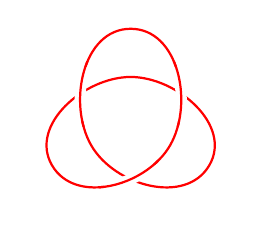
\begin{tikzpicture}
            \begin{knot}[
                consider self intersections,
                clip width=5
            ]
                \strand[red,thick] (1,{3^0.5})
                    to [out=0,in=60] (1.5,0.25)
                    to [out=240,in=-60] (0,0)
                    to [out=120,in=180] (1,1.12)
                    to [out=0,in=60] (2,0)
                    to [out=240,in=-60] (0.5,0.25)
                    to [out=120,in=180] cycle
                ;
                \flipcrossings{3}
            \end{knot}
        \end{tikzpicture}
        \caption{A projection of the unknot evoking the trefoil knot.}
        \label{fig:knottotrivial}
    \end{figure}
\end{itemize}


\subsection{Composition of Knots}\label{sss:Composition}
\begin{itemize}
    \item \textbf{Composition} (of two knots): \dq{A new knot obtained by removing a small arc from two knot projections and then connecting the four endpoints by two new arcs}{7}
    \begin{itemize}
        \item If two knots are designated $J$ and $K$, then their composition is denoted $J\#K$.
        \item Do not overlap the projections and choose two arcs that are on the outside to avoid new crossings.
        \item Make sure that the new arcs do not cross any of the the original knot projections or each other.
    \end{itemize}
    \item \textbf{Composite knot}: A knot that \dq{can be expressed as the composition of two knots, neither of which is the trivial knot}{8}
    \begin{itemize}
        \item This definition is analogous to composite integers, where an integer is \underline{composite} if it is the product of positive integers, neither of which is $1$.
        \item Similarly, if we compose any knot with the unknot, we get the same knot back.
    \end{itemize}
    \item \textbf{Factor knots}: \dq{The knots that make up the composite knot}{8}
    \item \textbf{Prime knot}: \dq{A knot [that] is not the composition of any two nontrivial knots}{9}
    \item The unknot, trefoil knot, and figure-eight knots are all prime (see Section \ref{sss:GenusSeifert}).
    \begin{itemize}
        \item The unknot is not composite for the same reason that 1 is not the product of two integers greater than 1.
    \end{itemize}
    \begin{figure}[h!]
        \centering
        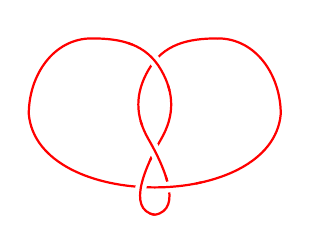
\begin{tikzpicture}[scale=0.8]
            \begin{knot}[
                clip width=5
            ]
                % Use looseness=# key to stretch out lengths!
                \strand[red,thick]       (0,0)
                    to [out=-85,in=-95]  (4,0)
                    to [out=90,in=0]     (3,1.2)
                ;
                \strand[red,thick]       (3,1.2)
                    to [out=180,in=60]   (1.9,0.7)
                    to [out=-120,in=120] (1.9,-0.4)
                    to [out=-60,in=10]   (2,-1.6)
                ;
                \strand[red,thick]       (2,-1.6)
                    to [out=170,in=-120] (2.1,-0.4)
                    to [out=60,in=-60]   (2.1,0.7)
                    to [out=120,in=0]    (1,1.2)
                    to [out=180,in=90]   (0,0)
                ;
                \flipcrossings{2,3}
            \end{knot}
        \end{tikzpicture}
        \caption{The figure-eight knot.}
        \label{fig:figure8knot}
    \end{figure}
    \item Similar to integers, \dq{a composite knot factors into a unique set of prime knots}{10}
    \item \emph{Exercise 1.8}: Using the appendix table, identify the factor knots that make up the composite knot in Figure \ref{fig:compos1}.
    \begin{itemize}
        \item The knot in Figure \ref{fig:compos1} is the composition of two projections of $5_2$.
    \end{itemize}
    \newpage
    \begin{figure}[h!]
        \centering
        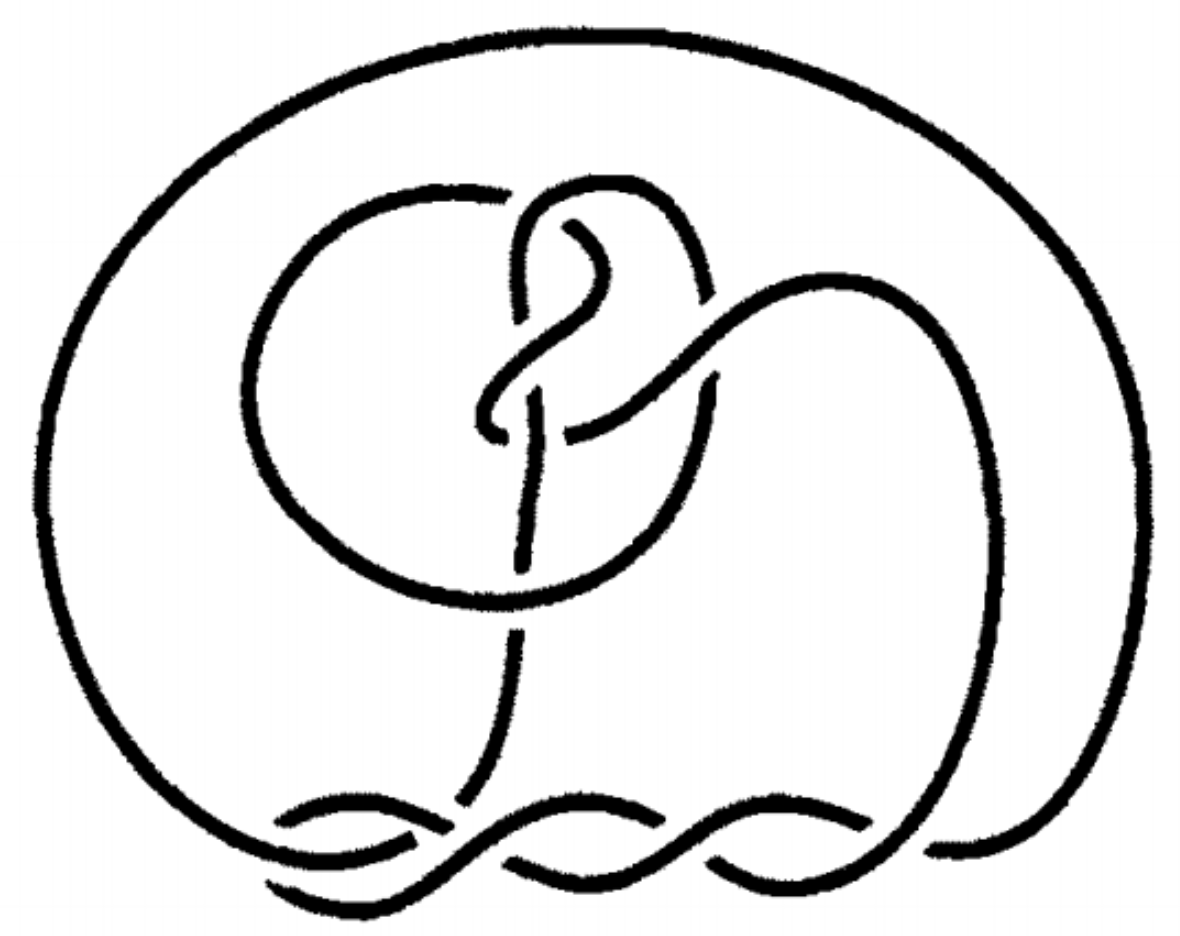
\includegraphics[width=0.2\linewidth]{Blender/compos1.png}
        \caption{The composite knot.}
        \label{fig:compos1}
    \end{figure}
    \item \emph{Exercise 1.9}: Show that the knot in Figure \ref{fig:compos2a} is composite.
    \begin{figure}[h!]
        \centering
        \begin{subfigure}[b]{0.3\textwidth}
            \centering
            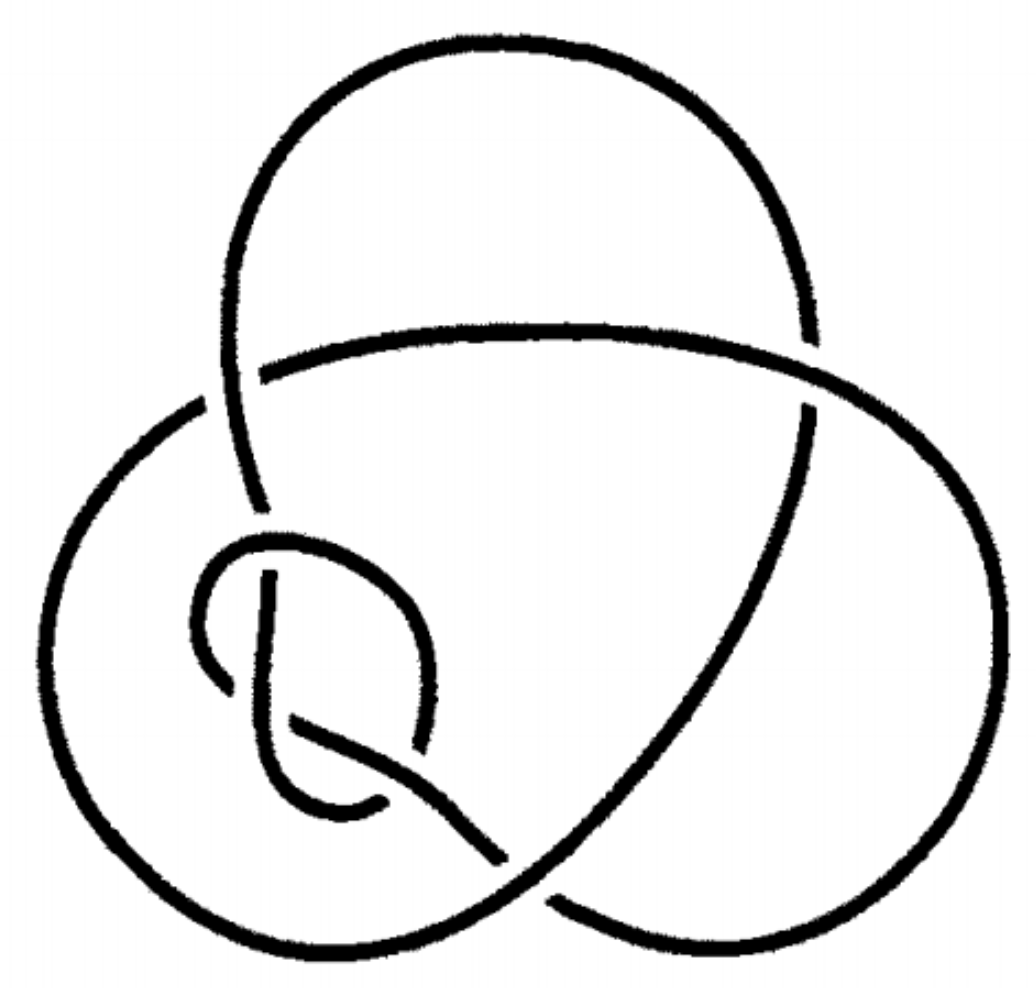
\includegraphics[width=0.5\textwidth]{Blender/compos2.png}
            \caption{The composite knot.}
            \label{fig:compos2a}
        \end{subfigure}
        \begin{subfigure}[b]{0.3\textwidth}
            \centering
            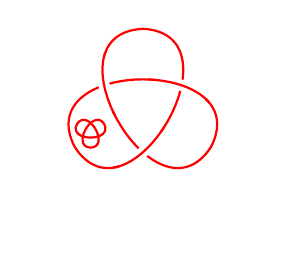
\begin{tikzpicture}
                \begin{knot}[
                    clip width=5,
                    consider self intersections
                ]
                    % Why don't polar coordinates mesh with figures?
                    \strand[red,thick] (90:1)
                        \foreach \x in {1,2,3} {
                            to [bend left=117,looseness=1.9] ({90+120*\x}:1)
                        }
                    ;
                    \flipcrossings{1,3}
                \end{knot}
                \begin{knot}[
                    clip width=5,
                    consider self intersections,
                    rotate=60,
                    scale=0.2,
                    xshift=-3cm,yshift=2.1cm
                ]
                    \strand[red,thick] (90:1)
                        \foreach \x in {1,2,3} {
                            to [bend left=117,looseness=1.9] ({90+120*\x}:1)
                        }
                    ;
                    \flipcrossings{1,3}
                \end{knot}
            \end{tikzpicture}
            \vspace{-0.8cm}
            \caption{Factors.}
            \label{fig:compos2b}
        \end{subfigure}
        \caption{Factorization of a `double trefoil.'}
        \label{fig:compos2}
    \end{figure}
    \item There is more than one way to take the composition of two knots (by removing different arcs).
    \begin{itemize}
        \item This is not analogous to multiplication --- a break in the pattern.
    \end{itemize}
    \item \textbf{Orientation}: A direction to travel around the knot. Denoted by placing \dq{coherently directed arrows along the projection of the knot in the direction of our choice}{10} A knot with such arrows is \textbf{oriented}.
    \begin{itemize}
        \item All compositions $J\#K$ where the orientations of $J$ and $K$ \underline{do} match up will yield the same composite knot.
        \begin{itemize}
            \item $J$ can be `slid around' $J\#K$ until it reaches the second position where the composition was taken.
        \end{itemize}
        \item All compositions $J\#K$ where the orientations of $J$ and $K$ \underline{do not} match up will yield the same composite knot.
        \item These two compositions can be distinct.
    \end{itemize}
    \begin{figure}[h!]
        \centering
        \begin{tikzpicture}
            \begin{knot}[
                clip width=5,
                consider self intersections
            ]
                \strand[red,thick,
                decoration={markings,
                mark=at position 0.2 with {\arrow{>}}},
                postaction={decorate}] (90:1)
                    \foreach \x in {1,2,3} {
                        to [bend left=117,looseness=1.9] ({90+120*\x}:1)
                    }
                ;
                \flipcrossings{1,3}
            \end{knot}
        \end{tikzpicture}
        \vspace{-0.8cm}
        \caption{Orientation notation.}
        \label{fig:orientnotation}
    \end{figure}
    \item \textbf{Invertible}: A knot that can be deformed back to itself so that an orientation on it is sent to the opposite orientation.
    \begin{itemize}
        \item \dq{In the case that one of the two knots is invertible, say $J$, we can always deform the composite knot so that the orientation on $K$ is reversed, and hence so that the orientations of $J$ and $K$ always match. Therefore, there is only one composite knot that we can construct from the two knots}{11}
    \end{itemize}
    \item To determine the possible compositions of knots, it is necessary to know which knots are invertible, but no general technique has yet been discovered.
\end{itemize}


\subsection{Reidemeister Moves}
\begin{itemize}
    \item \textbf{Ambient isotropy}: \dq{The movement of the string through three-dimensional space without letting it pass through itself}{12}
    \item \textbf{Planar isotropy}: A deformation of \dq{the projection plane as if it were made of ruber with the projection drawn upon it}{12}
    \begin{itemize}
        \item Stretching, squeezing, rotating, bending single arcs, etc.
    \end{itemize}
    \item \textbf{Reidemeister move}: \dq{One of three ways to change a projection of the knot that \emph{will} change the relation between the crossings}{13}
    \item \textbf{First Reidemeister move}: \dq{Put in or take out a twist in the knot}{13} See Figure \ref{fig:reidema}. \emph{Also known as} \textbf{type I Reidemeister move}.
    \item \textbf{Second Reidemeister move}: \dq{Either add two crossings or remove two crossings}{13} See Figure \ref{fig:reidemb}. \emph{Also known as} \textbf{type II Reidemeister move}.
    \item \textbf{Third Reidemeister move}: \dq{Slide a strand of the knot from one side of a crossing to the other side of the crossing}{13} See Figure \ref{fig:reidemc}. \emph{Also known as} \textbf{type III Reidemeister move}.
    \begin{itemize}
        \item Note that the crossings in Figure \ref{fig:reidem} can be reversed and the move will still be classified under the same category.
    \end{itemize}
    \begin{figure}[h!]
        \centering
        \begin{subfigure}[b]{0.3\linewidth}
            \centering
            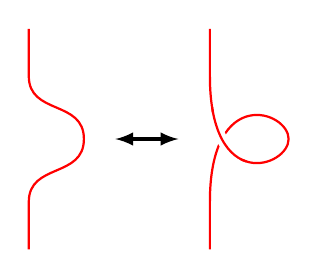
\begin{tikzpicture}
                \draw[red,thick,xshift=-1.5cm] (0,0.4) -- (0,1) .. controls (0,1.5) and (0.7,1.3) .. (0.7,1.8) .. controls (0.7,2.3) and (0,2.1) .. (0,2.6) -- (0,3.2);
                \draw[very thick,latex-latex] (-0.4,1.8) -- (0.4,1.8);
                \begin{knot}[
                    xshift=0.8cm,
                    consider self intersections=no splits,
                    clip width=5,
                    flip crossing=1
                ]
                    \strand[red,thick] (0,0.4) -- (0,1) to [out=90,in=90,out looseness=3,in looseness=0.7] (1,1.8) to [out=-90,in=-90,in looseness=3,out looseness=0.7] (0,2.6) -- (0,3.2);
                \end{knot}
            \end{tikzpicture}
            \caption{Type I Reidemeister move.}
            \label{fig:reidema}
        \end{subfigure}
        \begin{subfigure}[b]{0.3\linewidth}
            \centering
            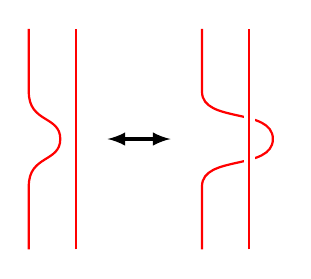
\begin{tikzpicture}
                \draw[red,thick,xshift=-1.4cm] (0,0.4) -- (0,1.2) .. controls (0,1.6) and (0.4,1.5) .. (0.4,1.8) .. controls (0.4,2.1) and (0,2) .. (0,2.4) -- (0,3.2);
                \draw[red,thick,xshift=-1.4cm] (0.6,0.4) -- (0.6,3.2);
                \draw[very thick,latex-latex] (-0.4,1.8) -- (0.4,1.8);
                \begin{knot}[
                    xshift=0.8cm,
                    clip width=5
                ]
                    \strand[red,thick] (0,0.4) -- (0,1.2) .. controls (0,1.6) and (0.9,1.4) .. (0.9,1.8) .. controls (0.9,2.2) and (0,2) .. (0,2.4) -- (0,3.2);
                    \strand[red,thick] (0.6,0.4) -- (0.6,3.2);
                    \flipcrossings{1,2}
                \end{knot}
            \end{tikzpicture}
            \caption{Type II Reidemeister move.}
            \label{fig:reidemb}
        \end{subfigure}\\
        \vspace{1em}
        \begin{subfigure}[b]{0.6\linewidth}
            \centering
            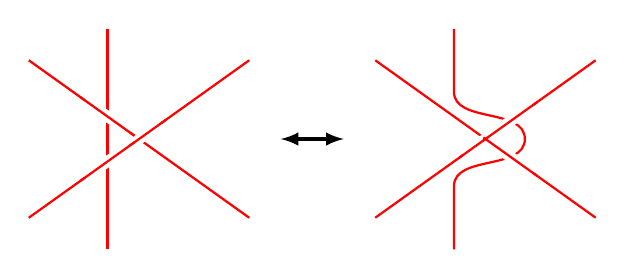
\begin{tikzpicture}
                \begin{knot}[
                    xshift=-2.2cm,
                    clip width=5
                ]
                    \strand[red,thick] (-1.4,0.8) -- (1.4,2.8);
                    \strand[red,thick] (-1.4,2.8) -- (1.4,0.8);
                    \strand[red,thick] (-0.4,0.4) -- (-0.4,3.2);
                \end{knot}
                \draw[very thick,latex-latex] (-0.4,1.8) -- (0.4,1.8);
                \begin{knot}[
                    xshift=2.2cm,
                    clip width=5
                ]
                    \strand[red,thick] (-1.4,0.8) -- (1.4,2.8);
                    \strand[red,thick] (-1.4,2.8) -- (1.4,0.8);
                    \strand[red,thick] (-0.4,0.4) -- (-0.4,1.2) .. controls (-0.4,1.6) and (0.5,1.4) .. (0.5,1.8) .. controls (0.5,2.2) and (-0.4,2) .. (-0.4,2.4) -- (-0.4,3.2);
                \end{knot}
            \end{tikzpicture}
            \caption{Type III Reidemeister move.}
            \label{fig:reidemc}
        \end{subfigure}
        \caption{Reidemeister moves.}
        \label{fig:reidem}
    \end{figure}
    \item All Reidemeister moves are ambient isotropies.
    \item \dq{If we have two distinct projections of the same knot, we can get from the one projection to the other by a series of Reidemeister moves and planar isotropies}{14}
    \item \textbf{Amphicheiral}: A knot that \dq{is equivalent to its mirror image, that is, the knot obtained by changing every crossing\dots to the opposite crossing}{14-15} \emph{Also known as} \textbf{achiral} \emph{by chemists.}
    \begin{itemize}
        \item A knot and its mirror image are distinct unless the knot is amphicheiral.
        \item See Section \ref{sse:biochemphys} for more on amphicheirality.
    \end{itemize}
    \newpage
    \item \emph{Exercise 1.10}: Show that the two projections in Figure \ref{fig:ex1-10} represent the same knot by finding a series of Reidemeister moves from one to the other.
    \begin{figure}[h!]
        \centering
        \begin{subfigure}[b]{0.2\linewidth}
            \centering
            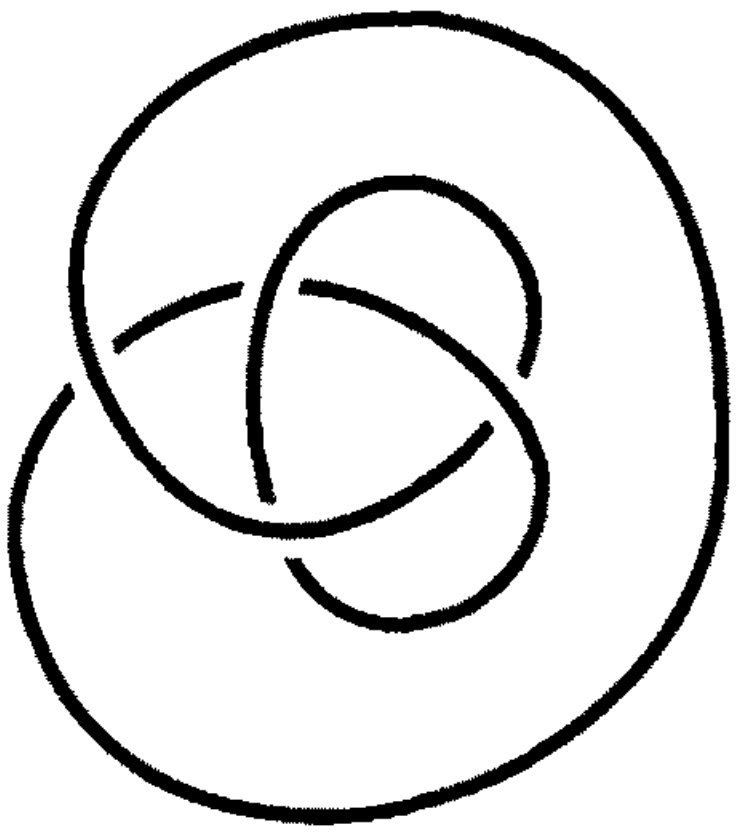
\includegraphics[width=0.6\linewidth]{Blender/ex1-10a.png}
            \caption{Initial projection.}
            \label{fig:ex1-10a}
        \end{subfigure}
        \begin{subfigure}[b]{0.2\linewidth}
            \centering
            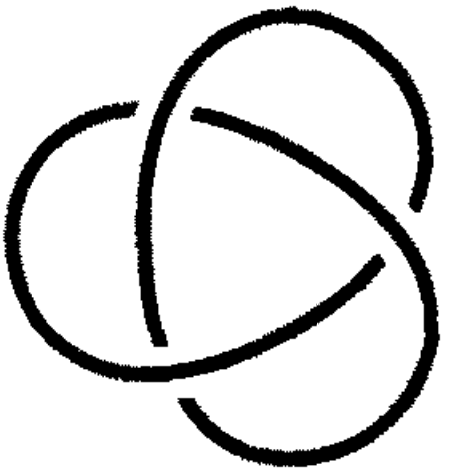
\includegraphics[width=0.4\linewidth]{Blender/ex1-10b.png}
            \vspace{4mm}
            \caption{Final projection.}
            \label{fig:ex1-10b}
        \end{subfigure}
        \caption{Finding Reidemeister moves.}
        \label{fig:ex1-10}
    \end{figure}
    \begin{figure}[h!]
        \centering
        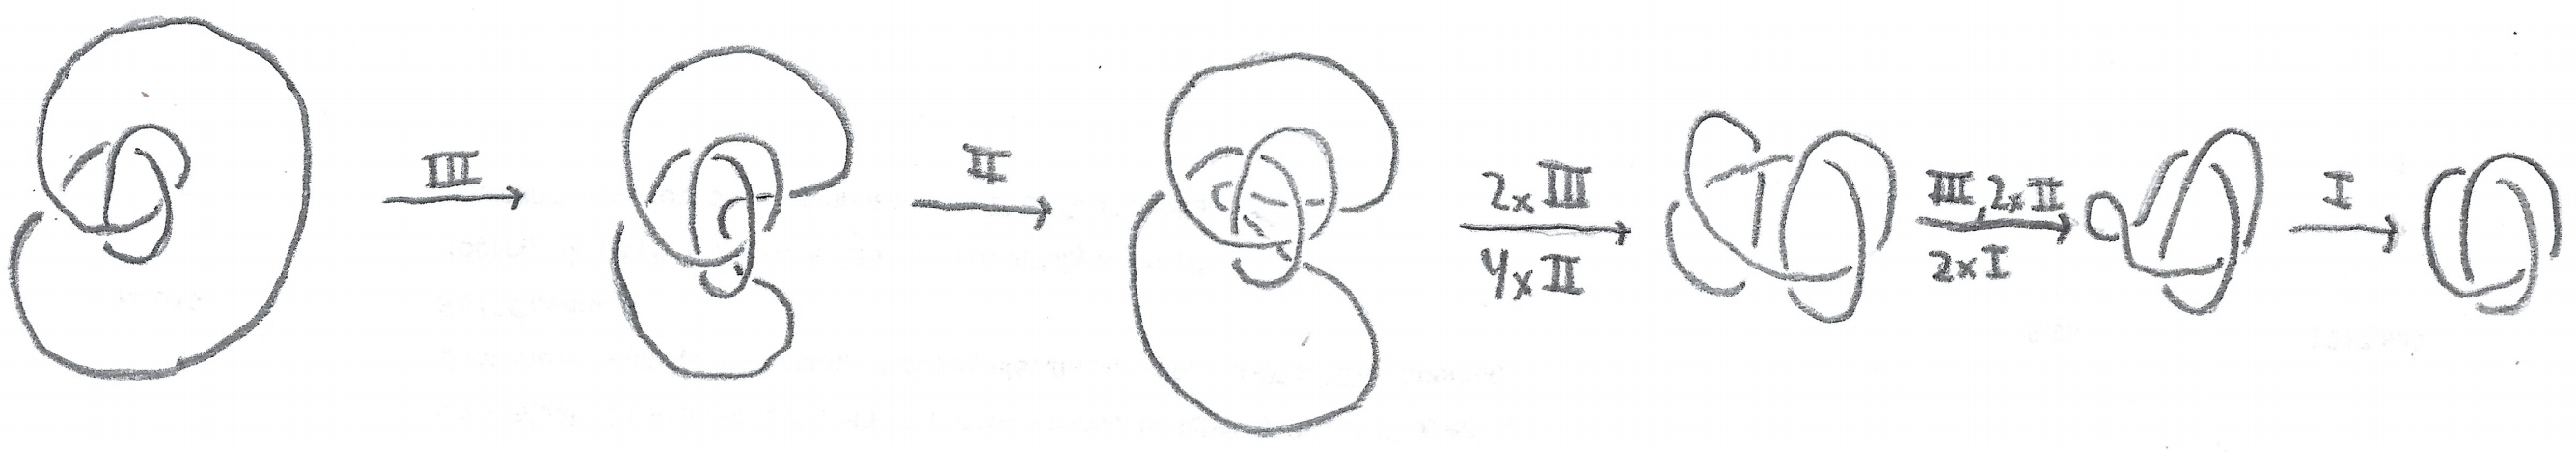
\includegraphics[width=0.8\linewidth]{Blender/ex1-10-2.png}
        \caption{Solution to \emph{Exercise 1.10}.}
        \label{fig:ex1-10-2}
    \end{figure}
    \item \emph{Exercise 1.11*}: Find a sequence of Reidemeister moves to untangle the unknot shown in Figure \ref{fig:ex1-11}.
    \begin{figure}[h!]
        \centering
        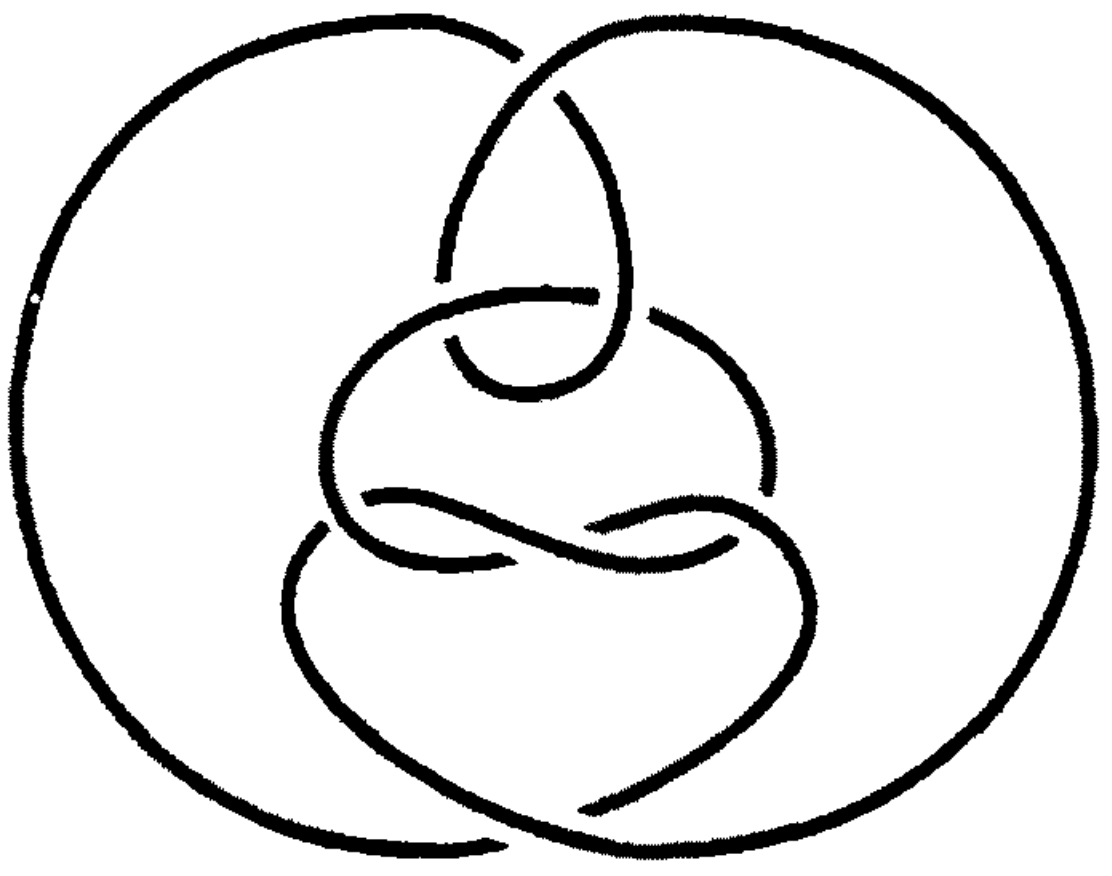
\includegraphics[width=0.17\linewidth]{Blender/ex1-11.png}
        \caption{Unknot to be untangled.}
        \label{fig:ex1-11}
    \end{figure}
    \begin{figure}[h!]
        \centering
        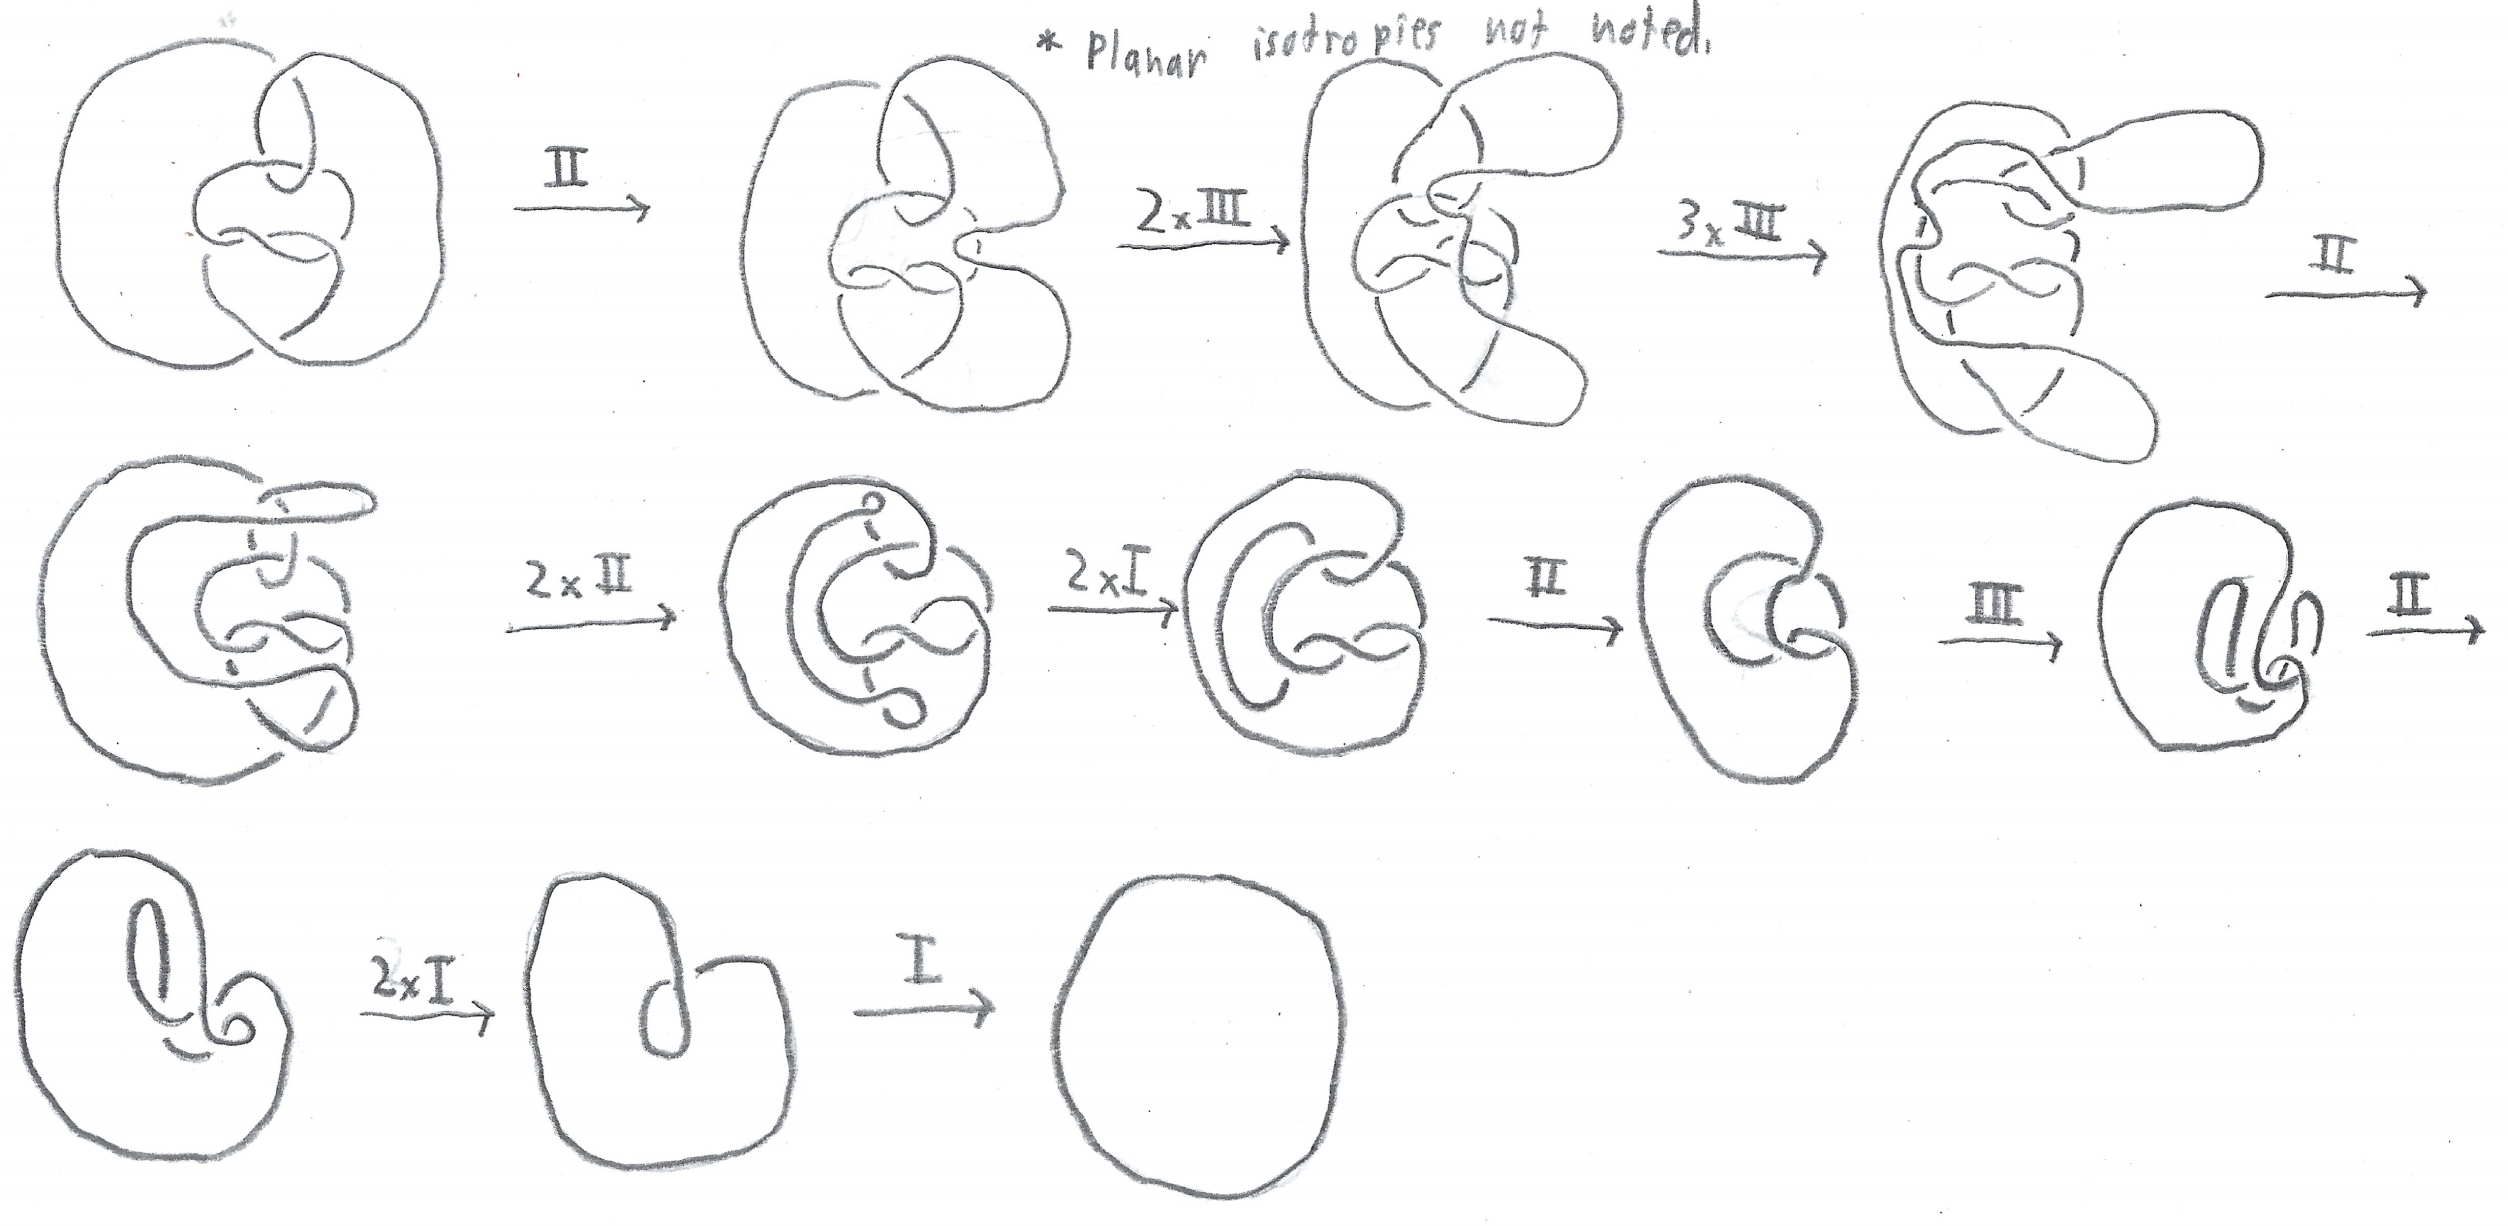
\includegraphics[width=0.8\linewidth]{Blender/ex1-11-2.png}
        \caption{Solution to \emph{Exercise 1.11*}.}
        \label{fig:ex1-11-2}
    \end{figure}
    \item The bounds on the increase in crossings generated by Reidemeister moves from one projection to another are unknown.
\end{itemize}


\subsection{Links}\label{sss:Links}
\begin{itemize}
    \item \textbf{Link}: \dq{A set of knotted loops all tangled up together}{17}
    \item \dq{Two links are considered to be the same if we can deform the one link to the other link without ever having any one of the loops intersect itself or any of the other loops in the process}{17}
    \begin{figure}[h!]
        \centering
        \begin{subfigure}[b]{0.2\linewidth}
            \centering
            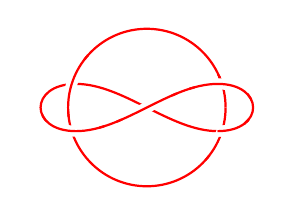
\begin{tikzpicture}
                \begin{knot}[
                    clip width=5,
                    ignore endpoint intersections=false,
                    consider self intersections=true
                ]
                    \strand[red,thick] circle (1cm);
                    \strand[red,thick] plot[smooth cycle,tension=1.2] coordinates{
                        (-0.9,0.3) (0.9,-0.3) (0.9,0.3) (-0.9,-0.3)
                    };
                    \flipcrossings{3,5}
                \end{knot}
            \end{tikzpicture}
            \caption{Whitehead link.}
            \label{fig:WhiteheadBorromeana}
        \end{subfigure}
        \begin{subfigure}[b]{0.2\linewidth}
            \centering
            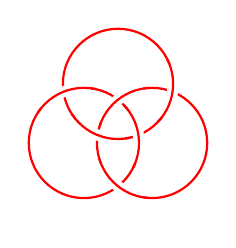
\begin{tikzpicture}
                \begin{knot}[
                    clip width=5
                ]
                    \strand[red,thick] (90:0.5)  circle (0.7cm);
                    \strand[red,thick] (210:0.5) circle (0.7cm);
                    \strand[red,thick] (330:0.5) circle (0.7cm);
                    \flipcrossings{1,2,5,6}
                \end{knot}
            \end{tikzpicture}
            \caption{Borromean rings.}
            \label{fig:WhiteheadBorromeanb}
        \end{subfigure}
        \caption{Projections of two common links.}
        \label{fig:WhiteheadBorromean}
    \end{figure}
    \item \emph{Exercise 1.13}: Show that the two projections in Figure \ref{fig:ex1-13a} and \ref{fig:ex1-13c} represent the same link.
    \begin{itemize}
        \item Untwist the right side of the figure-eight loop, twisting the right side of the circle at the same time. Then add a futher twist to the circle loop and flip (rotate along the horizontal axis) the figure-eight loop (which now looks like an ellipse).
    \end{itemize}
    \begin{figure}[h!]
        \centering
        \begin{subfigure}[b]{0.3\linewidth}
            \centering
            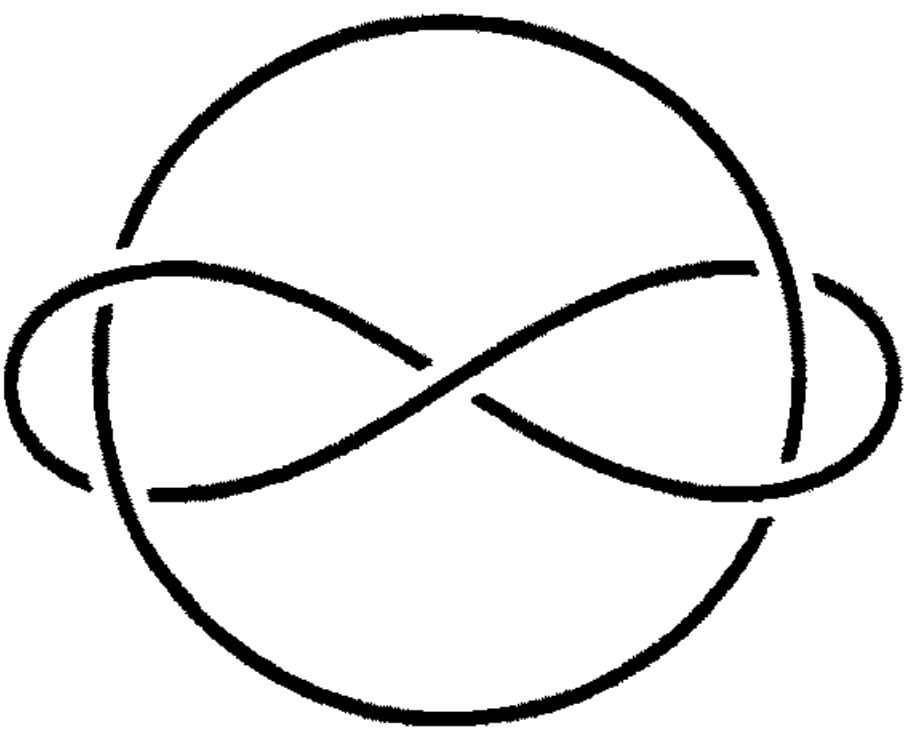
\includegraphics[width=0.5\linewidth]{Blender/ex1-13a.png}
            \caption{Initial projection.}
            \label{fig:ex1-13a}
        \end{subfigure}
        \begin{subfigure}[b]{0.3\linewidth}
            \centering
            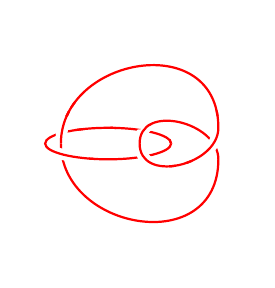
\begin{tikzpicture}
                \begin{knot}[
                    clip width=5,
                    consider self intersections=true,
                    ignore endpoint intersections=false
                ]
                    \strand[red,thick] (-0.4,0) ellipse (0.8cm and 0.2cm);
                    \strand[red,thick] (-1,0)
                        to [out=90,in=90,out looseness=1.4,in looseness=1.6] (1,0.2)
                        to [out=270,in=270,out looseness=1.2,in looseness=1.3] (0,0)
                        to [out=90,in=90,out looseness=1.3,in looseness=1.2] (1,-0.2)
                        to [out=270,in=270,out looseness=1.6,in looseness=1.4] cycle
                    ;
                    \flipcrossings{2,4,6}
                \end{knot}
            \end{tikzpicture}
            \vspace{-1em}
            \caption{Intermediate projection.}
            \label{fig:ex1-13b}
        \end{subfigure}
        \begin{subfigure}[b]{0.3\linewidth}
            \centering
            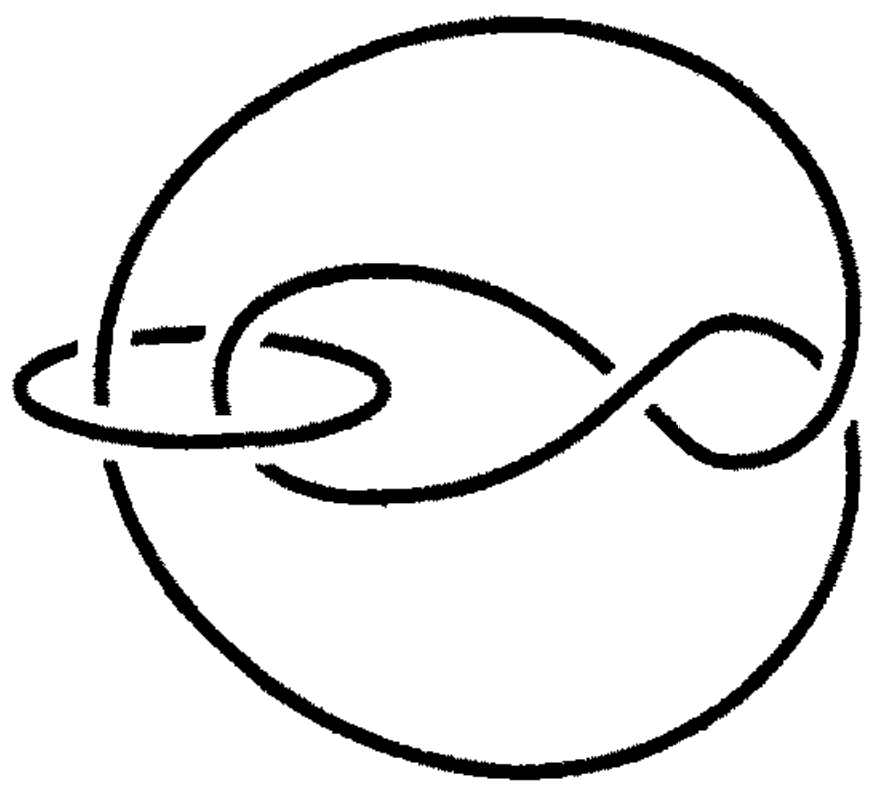
\includegraphics[width=0.5\linewidth]{Blender/ex1-13c.png}
            \caption{Final projection.}
            \label{fig:ex1-13c}
        \end{subfigure}
        \caption{Ambient isotropies of the Whitehead link.}
        \label{fig:ex1-13}
    \end{figure}
    \item \textbf{Link of \emph{n} components}: A link made up of $n$ loops knotted with each other.
    \begin{itemize}
        \item The Whitehead link (Figure \ref{fig:WhiteheadBorromeana}) is a \underline{link of 2 components}.
        \item The Borromean rings (Figure \ref{fig:WhiteheadBorromeanb}) are a \underline{link of 3 components}.
        \item A knot is a \underline{link of 1 component}.
        \item If the number of components in two links differ, then the links are clearly distinct.
    \end{itemize}
    \item \textbf{Splittable}: A link whose components \dq{can be deformed so that they lie on different sides of a plane in three-space}{17}
    \item \emph{Exercise 1.14}: Show that the link in Figure \ref{fig:ex1-14} is splittable.
    \begin{figure}[h!]
        \centering
        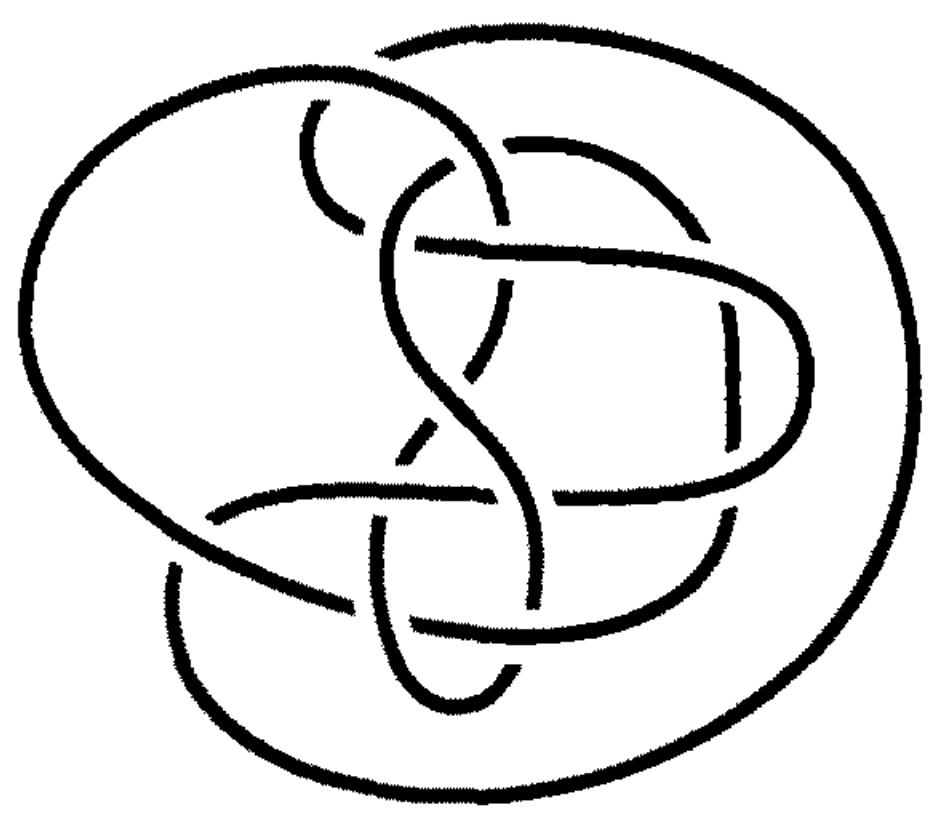
\includegraphics[width=0.2\linewidth]{Blender/ex1-14.png}
        \caption{Link to be split.}
        \label{fig:ex1-14}
    \end{figure}
    \begin{figure}[h!]
        \centering
        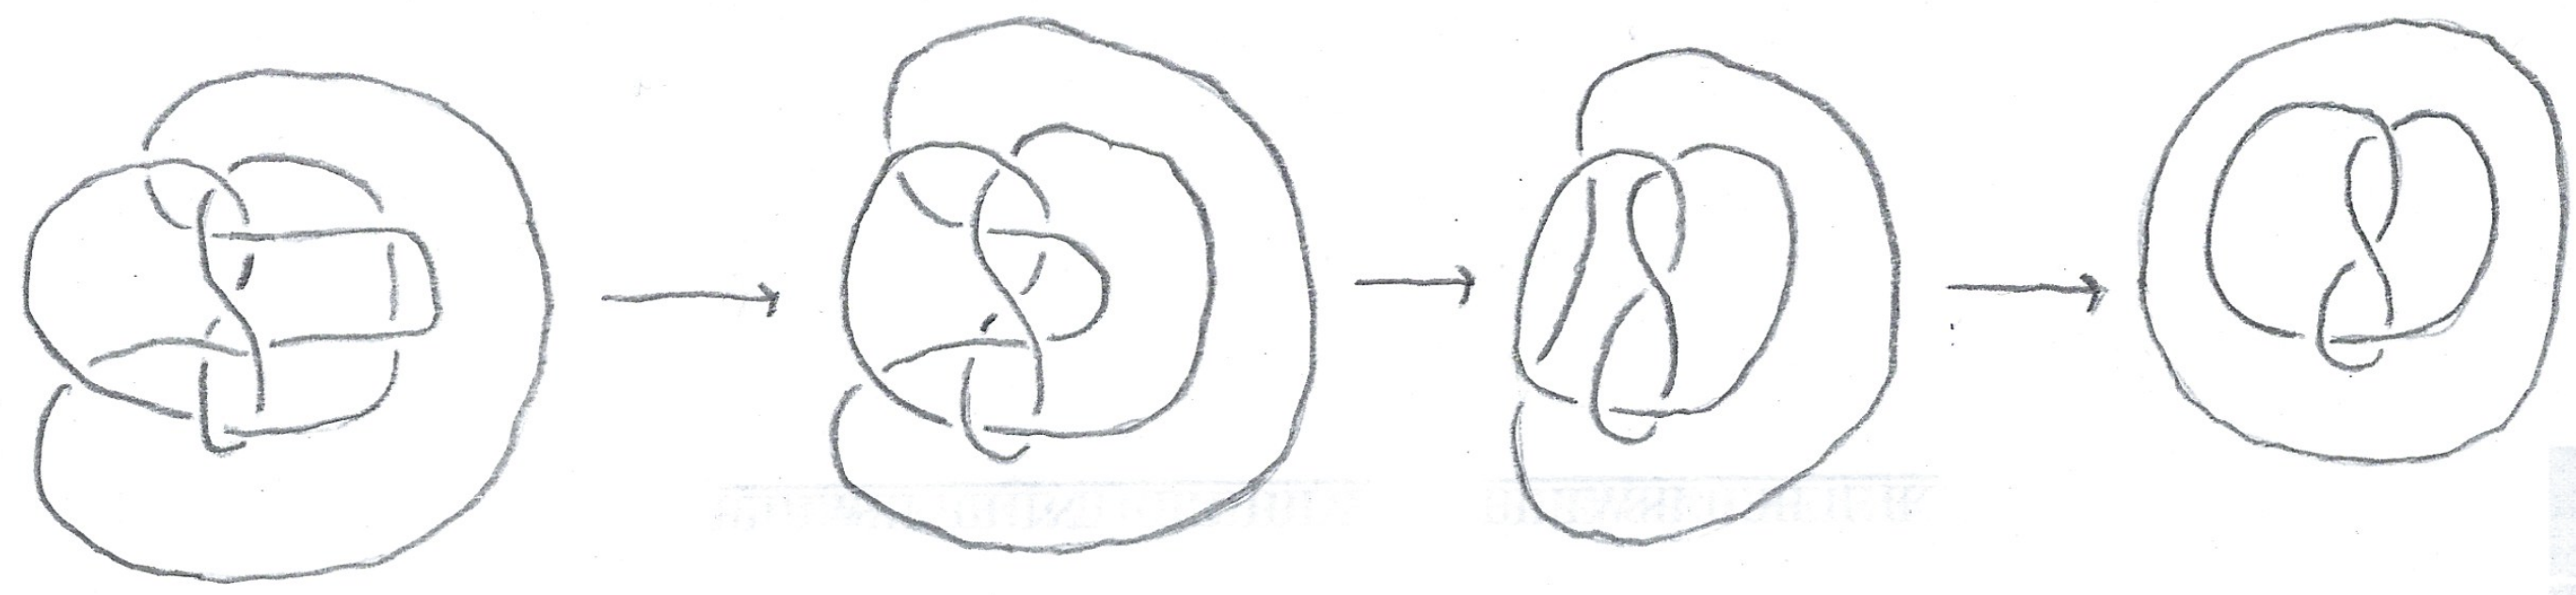
\includegraphics[width=0.8\linewidth]{Blender/ex1-14-2.png}
        \caption{Solution to \emph{Exercise 1.14}.}
        \label{fig:ex1-14-2}
    \end{figure}
    \item \textbf{Unlink}: One of the two simplest links of two components and the simplest splittable link of two components. \emph{Also known as} \textbf{trivial link}. See Figure \ref{fig:unlinkHopfa}.
    \item \textbf{Hopf link} The other of the two simplest links of two components and the simplest nonsplittable link of two components. See Figure \ref{fig:unlinkHopfb}.
    \begin{figure}[h!]
        \centering
        \begin{subfigure}[b]{0.4\linewidth}
            \centering
            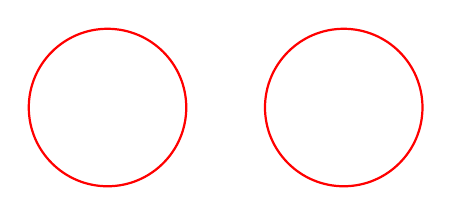
\begin{tikzpicture}[red,thick]
                \draw (-1.5,0) circle (1cm);
                \draw (1.5,0)  circle (1cm);
            \end{tikzpicture}
            \caption{Trivial link.}
            \label{fig:unlinkHopfa}
        \end{subfigure}
        \begin{subfigure}[b]{0.4\linewidth}
            \centering
            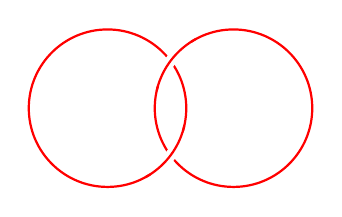
\begin{tikzpicture}
                \begin{knot}[
                    clip width=5,
                    flip crossing=1
                ]
                    \strand[red,thick] (-0.8,0) circle (1cm);
                    \strand[red,thick] (0.8,0)  circle (1cm);
                \end{knot}
            \end{tikzpicture}
            \caption{Hopf link.}
            \label{fig:unlinkHopfb}
        \end{subfigure}
        \caption{Projections of the two simplest links of two components.}
        \label{fig:unlinkHopf}
    \end{figure}
    \item \textbf{Linking number}: A quantity that numerically measures how linked up two components are.
    \begin{itemize}
        \item If $M$ and $N$ are two components in a link, begin by orienting both of them.
        \item At each crossing, count a $+1$ if Figure \ref{fig:linkingnumbera} holds or count a $-1$ if Figure \ref{fig:linkingnumberb} holds.
        \begin{itemize}
            \item Note that if you are unsure, do the following: If rotating the bottom strand clockwise lines up the arrows (correlates the two orientations), count $+1$.
            \item In the same vein, if rotating the bottom strand counterclockwise lines up the arrows, count $-1$.
            \item If a component crosses itself, do not count it.
        \end{itemize}
        \begin{figure}[h!]
            \centering
            \begin{subfigure}[b]{0.2\linewidth}
                \centering
                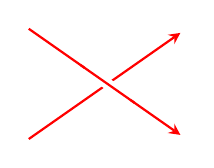
\begin{tikzpicture}
                    \begin{knot}[
                        clip width=5,
                        flip crossing=1
                    ]
                        \strand[red,thick,-stealth] (-1,-0.7) -- (1,0.7);
                        \strand[red,thick,-stealth] (-1,0.7) -- (1,-0.7);
                    \end{knot}
                \end{tikzpicture}
                \caption{Count $+1$.}
                \label{fig:linkingnumbera}
            \end{subfigure}
            \begin{subfigure}[b]{0.2\linewidth}
                \centering
                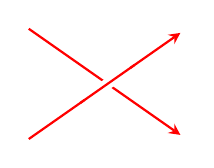
\begin{tikzpicture}
                    \begin{knot}[
                        clip width=5
                    ]
                        \strand[red,thick,-stealth] (-1,-0.7) -- (1,0.7);
                        \strand[red,thick,-stealth] (-1,0.7) -- (1,-0.7);
                    \end{knot}
                \end{tikzpicture}
                \caption{Count $-1$.}
                \label{fig:linkingnumberb}
            \end{subfigure}
            \caption{Computing linking numbers per crossing.}
            \label{fig:linkingnumber}
        \end{figure}
        \item Sum all of the $+1$s and $-1$s and divide this sum by 2 to yield the linking number.
        \begin{itemize}
            \item For example, the linking number for the Hopf link (Figure \ref{fig:unlinkHopfb}) is $\pm 1$ depending on the chosen orientation.
            \item Note that reversing the orientation for one of the two links is equivalent to multiplying the linking number by $-1$.
            \item As such, the absolute value of the linking number remains constant whatever orientation is chosen.
        \end{itemize}
    \end{itemize}
    \item \emph{Exercise 1.15}: Compute the linking number of the link pictured in Figure \ref{fig:ex1-15}. Now reverse the direction on one of the components and recompute it.
    \begin{itemize}
        \item Add up all of the numbers in the second row of Table \ref{tab:ex1-15} to yield $2$. Divide by $2$ to yield the linking number, $1$.
    \end{itemize}
    \begin{figure}[h!]
        \centering
        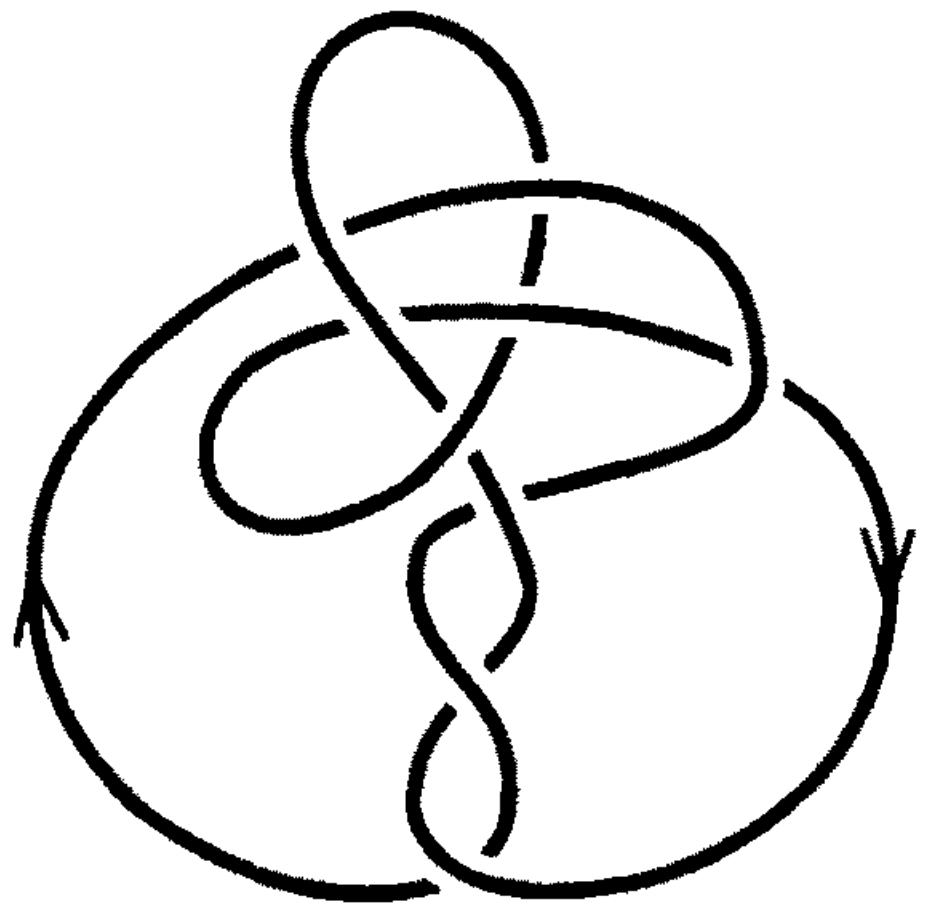
\includegraphics[width=0.2\linewidth]{Blender/ex1-15.png}
        \begin{tikzpicture}[
                remember picture,overlay,
                red,thin
            ]
            \draw (-1.5,2.6)   circle (4pt) node[right]{A};
            \draw (-2.28,2.42) circle (4pt) node[left] {B};
            \draw (-2.08,2.13) circle (4pt) node[left] {C};
            \draw (-1.56,2.16) circle (4pt) node[right]{D};
            \draw (-0.73,1.96) circle (4pt) node[right]{E};
            \draw (-1.78,1.76) circle (4pt) node[right]{F};
            \draw (-1.65,1.48) circle (4pt) node[right]{G};
            \draw (-1.74,0.83) circle (4pt) node[right]{H};
            \draw (-1.77,0.15) circle (4pt) node[right]{I};
        \end{tikzpicture}
        \caption{Link of linking number $n$.}
        \label{fig:ex1-15}
    \end{figure}
    \renewcommand{\arraystretch}{1.4}
    \begin{table}[h!]
        \centering
        \begin{tabular}{|c|c|c|c|c|c|c|c|c|}
            \hline
            A    & B    & C   & D   & E    & F   & G    & H    & I   \\
            \hline
            $-1$ & $-1$ & $0$ & $0$ & $+1$ & $0$ & $+1$ & $+1$ & $+1$\\
            \hline
        \end{tabular}
        \caption{Counting crossings.}
        \label{tab:ex1-15}
    \end{table}
    \item Although a linking number is computed using a single projection of a link, the linking number will be the same for any projection of the link.
    \begin{itemize}
        \item This can be proven by demonstrating that the Redemeister moves do not change the linking number. \dq{Since we can get from any one projection of a link to any other via a sequence of Reidemeister moves, none of which will change the linking number, it must be that two different projections of the same link yield the same linking number}{20}
        \item Let's take this case by case.
        \begin{itemize}
            \item A Type I Reidemeister move generates a self-intersection. Because self-crossings do not count toward the linking number by definition, the first Reidemeister move does not affect the linking number.
            \item A Type II Reidemeister move generates two crossings. There are now two cases: Either the new crossings are self-intersections or they are not. If the new crossings are self-intersections, then there is no change to the linking number. If the new crossings are not self-intersections, they will always have opposite linking numbers, and, thus, the two new crossings cancel each other out. Therefore, the second Reidemeister move does not affect the linking number.
            \item A Type III Reidemeister move removes two crossings and generates two crossings. There are now two cases: Either the new crossings are self-intersections or they are not. If the new crossings are self-intersections, then there is no change to the linking number. If the new crossings are not self-intersections, both pairs of crossings will always have opposite linking numbers and, thus, both pairs of crossings cancel each other out. Therefore, the third Reidemeister move does not affect the linking number.
        \end{itemize}
        \item This logic can be visually confirmed by assigning orientations and counting crossings in Figure \ref{fig:reidem}.
    \end{itemize}
    \item \textbf{Invariant}: A quality of a knot or link that, once orientations are chosen, is unchanged by ambient isotropy.
    \begin{itemize}
        \item Both the linking number and the number of components are \underline{link invariants}.
    \end{itemize}
    \item \emph{Exercise 1.16}: Explain why the linking number of a splittable two-component link will always be $0$, no matter what projection is used to compute it.
    \begin{itemize}
        \item \textsc{Solution 1}: By definition, the linking number numerically measures how linked up two components are. Since splittable links are not joined (or "linked up") in any way, the linking number must be $0$.
        \item \textsc{Solution 2}: If a two-component link is splittable, then there exists a projection of it with no crossings that are not self-intersections (a projection of the split link, as in Figure \ref{fig:unlinkHopfb}). If all crossings are self-intersections, then the linking number computed for this projection must be $0$. Now that it is known that said link has a linking number of $0$, any combination of Reidemeister moves can be used to manipulate the link into any other projection. But because Reidemeister moves do not affect the linking number, the linking number will remain $0$.
    \end{itemize}
    \item The absolute value of the linking number, as a link invariant, can be used to distinguish certain distinct links, regardless of orientation.
    \begin{itemize}
        \item \dq{Any two links with two components that have distinct absolute values of their linking numbers have to be different links}{21}
        \item For example, the difference in linking number between the unlink (0; Figure \ref{fig:unlinkHopfa}) and the Hopf link (1; Figure \ref{fig:unlinkHopfb}) distinguishes them.
    \end{itemize}
    \item However, the linking number cannot distinguish between all links.
    \begin{itemize}
        \item For instance, both the Whitehead link (Figure \ref{fig:WhiteheadBorromeana}) and the unlink (Figure \ref{fig:unlinkHopfa}) have linking number 0.
        \item One such distinction is discussed in Section \ref{sss:tricolor}.
    \end{itemize}
    \item \textbf{Brunnian link}: A nontrivial link where the removal of any one component leaves behind a set of trivial unlinked circles.
    \begin{itemize}
        \item The Borromean rings (Figure \ref{fig:WhiteheadBorromeanb}) are Brunnian$^[$\footnote{How can I draw a Brunnian link with four components? Or more?}$^]$.
    \end{itemize}
\end{itemize}


\subsection{Tricolorability}\label{sss:tricolor}
\begin{itemize}
    \item How do we \emph{prove} that every knot is not just a projection of the unknot?
    \item \textbf{Strand}: \dq{A piece of the link that goes from one undercrossing to another with only overcrossings in between}{23}
    \item \textbf{Tricolorable}: A projection of a knot or link in which each strand \dq{can be colored one of three different colors, so that at each crossing, either three different colors come together or all the same color comes together}{23}
    \begin{figure}[h!]
        \centering
        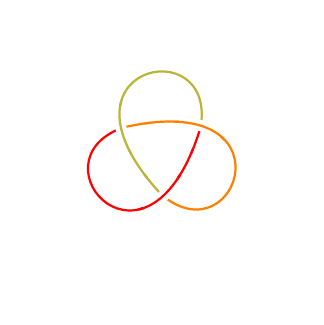
\begin{tikzpicture}
            \coordinate (a) at (30:0.57);
            \coordinate (b) at (150:0.57);
            \coordinate (c) at (270:0.57);
        
            \begin{knot}[
                clip width=5,clip radius=8pt,ignore endpoint intersections=false
            ]
                \strand[red,thick] (a) to[relative,out=73,in=20,out looseness=5.8,in looseness=3.3] (b);
                \strand[orange,thick] (b) to[relative,out=73,in=20,out looseness=5.8,in looseness=3.3] (c);
                \strand[yellow!70!black,thick] (c) to[relative,out=73,in=20,out looseness=5.8,in looseness=3.3] (a);
                \flipcrossings{1,3,5}
                \redraw{1}{(c)}
            \end{knot}
        \end{tikzpicture}
        \vspace{-0.8cm}
        \caption{Tricolored trefoil.}
        \label{fig:TricolorTrefoil}
    \end{figure}
    \item \emph{Exercise 1.21}: Determine which of the projections of the three six-crossing knots $6_1$, $6_2$, and $6_3$ are tricolorable.
    \begin{itemize}
        \item $6_1$ is tricolorable and the other two knots are not. I determined this through trial and error.
    \end{itemize}
    \item \emph{Exercise 1.22}: Show that the projection of the knot $7_4$ in Figure \ref{fig:ex1-22a} is tricolorable.
    \begin{figure}[h!]
        \centering
        \begin{subfigure}[b]{0.3\linewidth}
            \centering
            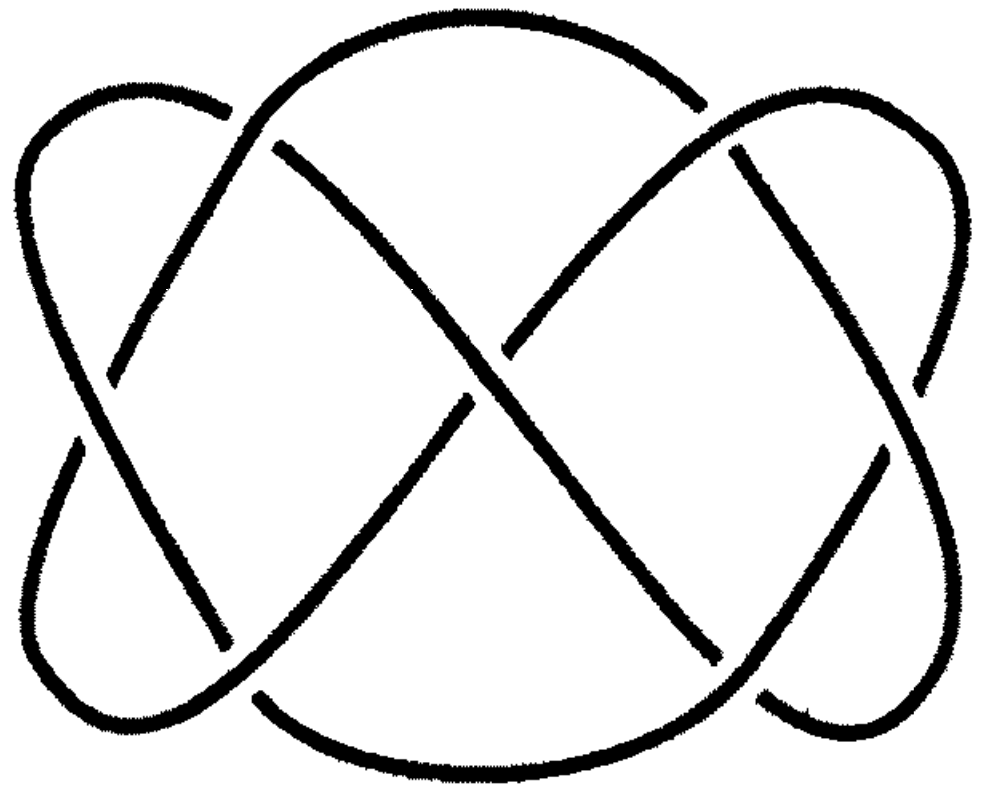
\includegraphics[width=0.5\linewidth]{Blender/ex1-22.png}
            \caption{Initial projection.}
            \label{fig:ex1-22a}
        \end{subfigure}
        \begin{subfigure}[b]{0.3\linewidth}
            \centering
            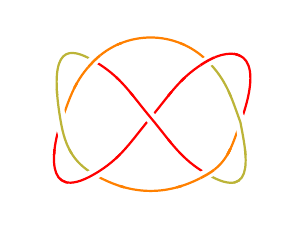
\begin{tikzpicture}[scale=0.6]
                \coordinate (a) at (-1.2,0.5);
                \coordinate (b) at (1.2,0.5);
                \coordinate (c) at (1.9,1.6);
                \coordinate (d) at (1.2,2.9);
                \coordinate (e) at (0,1.7);
                \coordinate (f) at (-1.9,1.6);
                \coordinate (g) at (-1.2,2.9);
                
                \begin{knot}[
                    clip width=5,
                    ignore endpoint intersections=false
                ]
                    \strand[orange,thick] (a)
                        to [out=-30,in=-150] (b)
                        to [out=30,in=-110] (c)
                    ;
                    \strand[red,thick] (c)
                        to [out=70,in=30,out looseness=3] (d)
                        to [out=-150,in=50] (e)
                    ;
                    \strand[red,thick] (e)
                        to [out=-130,in=30] (a)
                        to [out=-150,in=-110,out looseness=2.5] (f)
                    ;
                    \strand[orange,thick] (f)
                        to [out=70,in=-135] (g)
                        to [out=45,in=135] (d)
                    ;
                    \strand[yellow!70!black,thick] (d)
                        to [out=-45,in=110] (c)
                        to [out=-80,in=-30,in looseness=2.5] (b)
                    ;
                    \strand[red,thick] (b)
                        to [out=150,in=-50] (e)
                        to [out=130,in=-30] (g)
                    ;
                    \strand[yellow!70!black,thick] (g)
                        to [out=150,in=100,in looseness=3] (f)
                        to [out=-80,in=150] (a)
                    ;
                    \flipcrossings{10,13,19}
                \end{knot}

                \begin{scope}
                    \path[clip] (b) circle (5pt);
                    \draw[white,double=orange,very thick,double distance=0.9pt] (a)
                        to [out=-30,in=-150] (b)
                        to [out=30,in=-110] (c)
                    ;
                \end{scope}
                \begin{scope}
                    \path[clip] (d) circle (5pt);
                    \draw[white,double=red,very thick,double distance=0.9pt] (c)
                        to [out=70,in=30,out looseness=3] (d)
                        to [out=-150,in=50] (e)
                    ;
                \end{scope}
                \begin{scope}
                    \path[clip] (g) circle (5pt);
                    \draw[white,double=orange,very thick,double distance=0.9pt] (f)
                        to [out=70,in=-135] (g)
                        to [out=45,in=135] (d)
                    ;
                \end{scope}
            \end{tikzpicture}
            \caption{Tricolored projection.}
            \label{fig:ex1-22b}
        \end{subfigure}
        \caption{Tricolored $7_4$.}
        \label{fig:ex1-22}
    \end{figure}
    \item Reidemeister moves do not affect tricolorability.
    \begin{itemize}
        \item A Type I Reidemeister move generates a self-intersection. At such a crossing (made out of one original strand), every color will be the same; only one color meets at the crossing.
        \item A Type II Reidemeister move generates two crossings. If the strands are the same color, then everything stays the same color. If the strands are different colors, than newly created loop takes on the third color.
        \item Type III has many cases (\emph{Exercise 1.23}).
    \end{itemize}
    \item Since the unknot is not tricolorable and the trefoil knot is, we have just proven that there is at least one other knot besides the unknot.
    \begin{itemize}
        \item Tricolorability is a knot invariant.
    \end{itemize}
    \item For links, tricolorability is a bit different --- the unlink, for example, is tricolorable.
    \begin{figure}[h!]
        \centering
        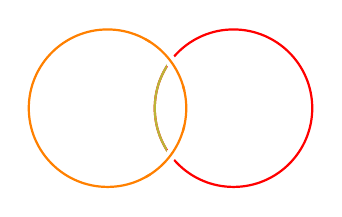
\begin{tikzpicture}
            \begin{knot}[
                clip width=5
            ]
                \strand[orange,thick] (-0.8,0) circle (1cm);
                \strand[red,thick] (0.8,0)  circle (1cm);
            \end{knot}
            \begin{scope}
                \clip (-0.045,-1) rectangle (-1.8,1);
                \draw[yellow!70!black,thick] (0.8,0) circle (1cm);
            \end{scope}
        \end{tikzpicture}
        \caption{Tricolored unlink.}
        \label{fig:tricolorUnlink}
    \end{figure}
\end{itemize}


\subsection{Knots and Sticks}
\begin{itemize}
    \item We can also consider knots made out of straight sticks glued to each other at each end.
    \item The first nontrivial knot made out of sticks is the trefoil, with six sticks.
    \begin{itemize}
        \item We know that the stick trefoil in Figure \ref{fig:sticktrefoil} could be made in the real world because, if two vertices lie in the $xy$-plane, then two lie above and two lie below.
        \item This P(lanar), L(ow), H(igh) notation is commonly used.
    \end{itemize}
    \begin{figure}[h!]
        \centering
        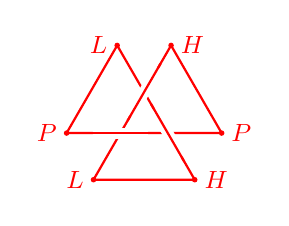
\begin{tikzpicture}
            \begin{knot}[
                clip width=5,
                consider self intersections
            ]
                \strand[red,thick] (70:1) to (-10:1) to (-170:1) to (110:1) to (-50:1) to (-130:1) to cycle;
                \flipcrossings{1,3}
            \end{knot}

            \fill[red] (70:1)   circle (1pt) node[right]{\small$H$};
            \fill[red] (-10:1)  circle (1pt) node[right]{\small$P$};
            \fill[red] (-170:1) circle (1pt) node[left] {\small$P$};
            \fill[red] (110:1)  circle (1pt) node[left] {\small$L$};
            \fill[red] (-50:1)  circle (1pt) node[right]{\small$H$};
            \fill[red] (-130:1) circle (1pt) node[left] {\small$L$};
        \end{tikzpicture}
        \caption{A trefoil knot made of sticks.}
        \label{fig:sticktrefoil}
    \end{figure}
    \item \textbf{Stick number}: \dq{The least number of straight sticks necessary to make a knot $K$}{29} \emph{Also known as} \textbf{s(K)}.
    \item The stick number for the composition of $n$ trefoil knots is $2n+4$.
    \item Many problems listed$^[$\footnote{These could make good topics for a larger paper. Alternatively, some I am not ready to solve and need to learn more math first (those that I will come back to at the end of the book). I do not believe I'm missing anything essential by skipping these for now, but we'll see.}$^]$.
\end{itemize}
\newpage



\section{Tabulating Knots}\label{sse:tabulating}
\subsection{History of Knot Tabulation}
\begin{itemize}
    \item Although many mathematicians (including Gauss) had dabbled with knots, Lord Kelvin's theory that atoms were knotted vortices in the ether (referenced in Section \ref{sss:Introduction}) kicked off research in earnest.
    \item Reverand Thomas P. Kirkman began tabulating knots but wrote poorly.
    \item However, Kirkman's ideas were applied by Scottish physicist Peter Guthrie Tait to list all alternating knots up to 10 crossings.
    \item C. N. Little of the University of Nebraska was the first to tackle the nonalternating knots.
    \begin{itemize}
        \item He tabulated up to 10 crossings (43 knots total).
        \item However, in 1974, it was discovered that two knots were, in fact, the same and there were really 42 knots.
        \begin{itemize}
            \item Kenneth A. Perko, a parttime mathematician and New York lawyer, discovered that the projections were not distinct. As such, the projections are known as the Perko pair (Figure \ref{fig:perkopair}).
        \end{itemize}
    \end{itemize}
    \item \emph{Exercise 2.1}: Show that the Perko pair (projected in Figure \ref{fig:perkopair}) are the same knot.
    \begin{figure}[h!]
        \centering
        \begin{subfigure}[b]{0.2\linewidth}
            \centering
            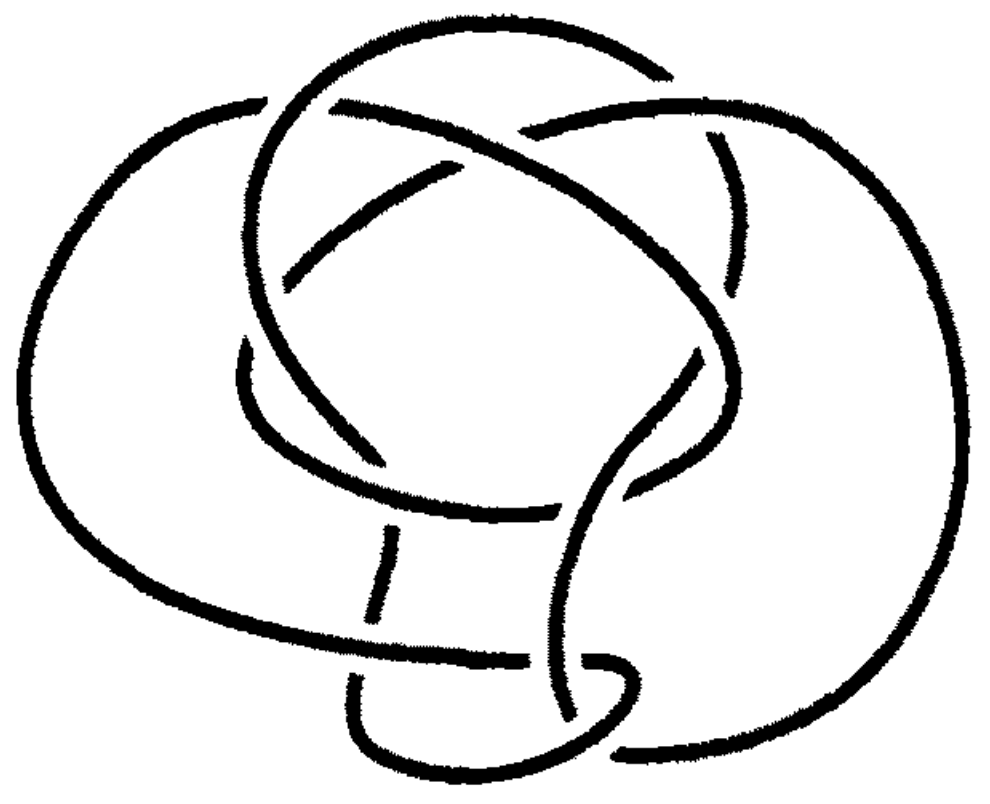
\includegraphics[width=0.8\linewidth]{Blender/perkopair1.png}
            \caption{Projection 1.}
            \label{fig:perkopaira}
        \end{subfigure}
        \begin{subfigure}[b]{0.2\linewidth}
            \centering
            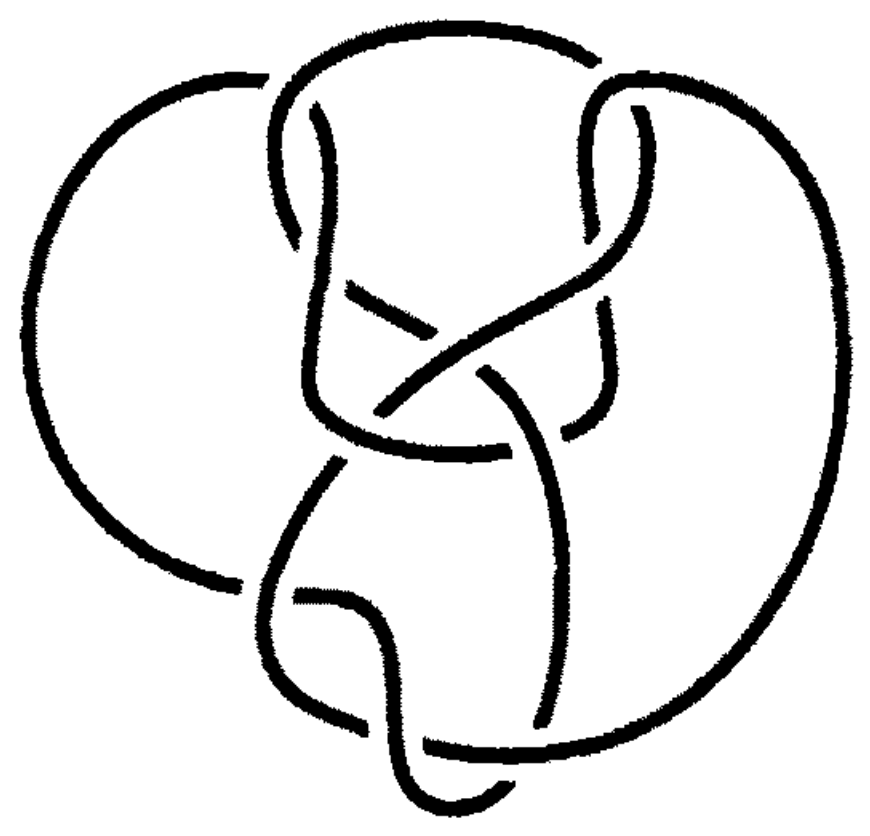
\includegraphics[width=0.7\linewidth]{Blender/perkopair2.png}
            \caption{Projection 2.}
            \label{fig:perkopairb}
        \end{subfigure}
        \caption{The Perko pair.}
        \label{fig:perkopair}
    \end{figure}
    \begin{figure}[h!]
        \centering
        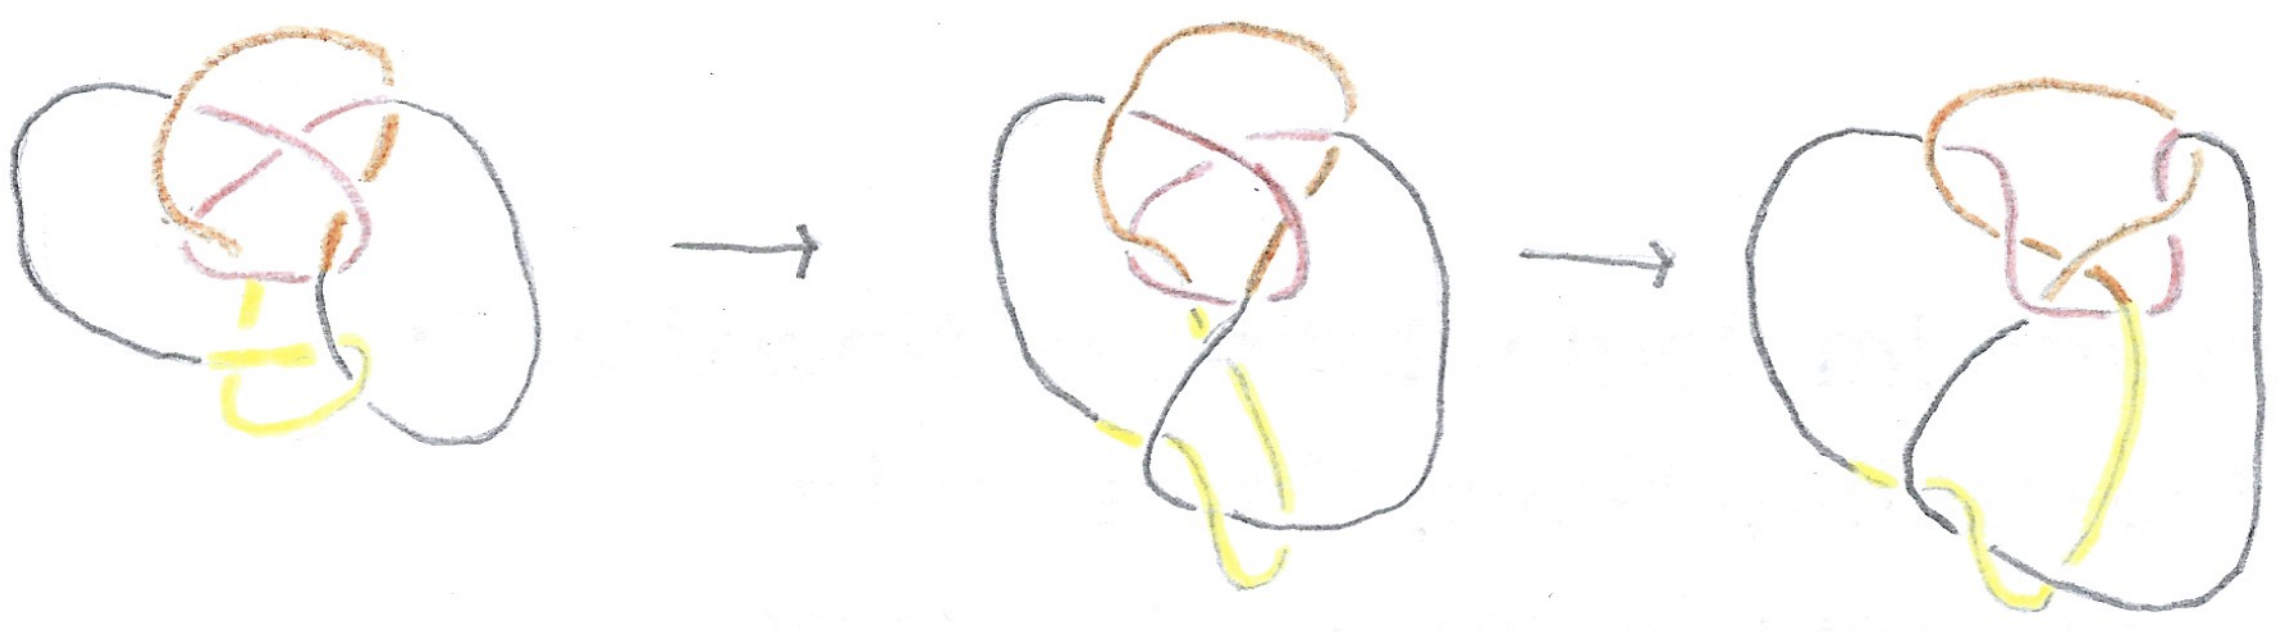
\includegraphics[width=0.6\linewidth]{Blender/ex2-1.png}
        \caption{Solution to \emph{Exercise 2.1}.}
        \label{fig:ex2-1}
    \end{figure}
    \item Little later published a census of 11-crossing alternating knots with 11 omissions and 1 duplication.
    \item Mary G. Haseman listed all amphicheiral knots of 12 crossings.
    \item Early on, there were few attempts to \emph{prove} that the tabulated knots were actually distinct.
    \item In 1927, Alexander and Briggs proved that the knots up to 9 crossings were distinct.
    \begin{itemize}
        \item They developed the first knot polynomial, the Alexander polynomial.
        \item This would remain the only knot polynomial until 1984.
    \end{itemize}
    \item Once Kurt Reidemeister finished rigorously classifying the knots up to 9 crossings in 1932, tabulation was inactive for a while.
    \item In 1969, John H. Conway developed a new notation and used it to determine all of the prime knots up to 11 crossings and all prime nonsplittable links up to 10 crossings.
    \item In 1978, Alain Caudron of the University of Paris corrected Conway's tabulation a bit.
    \item Meanwhile, a new notation was developed by Hugh Dowker (see Section \ref{sss:Dowker}) that was implemented as a computer algorithm by Morwen Thistlethwaite.
    \item In the 1980s-1990s (with computer help), Jim Hoste, Thistlethwaite, and Jeff Weeks (an expert in hyperbolic knots; see Section \ref{sss:Hyperbolic}) tabulated up to 16-crossing knots.
    \begin{itemize}
        \item Note that the number of knots of successive numbers of crossings \emph{appears} to grows exponentially (this is unproven).
        \item Also note that Hoste et al's listed knots includes those that are not amphicheiral only once, so those knots actually represent 2 distinct knots.
        \begin{itemize}
            \item Determining amphicheirality is discussed in Section \ref{sse:polynomials}
        \end{itemize}
    \end{itemize}
    \item On drawing a 14-crossing knot.
    \item Claus Ernst and Dewitt Sumners proved a lower exponential bound on the number of distinct prime knots (see Section \ref{sss:Bridge}).
    \item Dominic Welsh proved an upper exponential bound on the number of distinct prime knots.
\end{itemize}


\subsection{The Dowker Notation for Knots}\label{sss:Dowker}
\begin{itemize}
    \item For alternating knots\dots
    \begin{itemize}
        \item Begin by choosing an orientation.
        \item Label an arbitrary crossing 1.
        \item Leaving that crossing on the understrand, label the next crossing 2.
        \item Continue through the crossing on the same strand and label the next crossing 3.
        \item Continue in this fashion until you have gone all the way around the knot once.
        \begin{itemize}
            \item Note that this gives each crossing two numbers.
        \end{itemize}
    \end{itemize}
    \begin{figure}[h!]
        \centering
        \begin{tikzpicture}
            \begin{knot}[
                clip width=5,
                consider self intersections
            ]
                \strand[red,thick,
                decoration={markings,
                mark=at position 0.2 with {\arrow{>}}},
                postaction={decorate}] (90:1)
                    \foreach \x in {1,2,3} {
                        to [bend left=117,looseness=1.9] ({90+120*\x}:1)
                    }
                ;
                \flipcrossings{1,3}
            \end{knot}
            \footnotesize
            \fill (30:0.57) circle (0pt)
                node[above right]{1}
                node[below left]{4}
            ;
            \fill (-90:0.57) circle (0pt)
                node[above]{2}
                node[below]{5}
            ;
            \fill (150:0.57) circle (0pt)
                node[above right]{3}
                node[below left=]{6}
            ;
            \normalsize
        \end{tikzpicture}
        \caption{Trefoil knot labeled in Dowker notation.}
        \label{fig:Dowkertrefoil}
    \end{figure}
    \item \emph{Exercise 2.2}: Why does every crossing get one even numbered label and one odd numbered label?
    \begin{itemize}
        \item Because the knot is alternating --- every understrand will add an odd label and every overstrand will add an even number (because you set off on the understrand after labeling your starter crossing 1).
    \end{itemize}
    \begin{table}[h!]
        \centering
        \begin{tabular}{ccc}
            1 & 3 & 5\\
            4 & 6 & 2
        \end{tabular}
        \caption{Dowker numerical pairing of a trefoil knot.}
        \label{tab:Dowkertrefoil}
    \end{table}
    \item From the counting in Figure \ref{fig:Dowkertrefoil}, we obtain a pairing between the numbers (Table \ref{tab:Dowkertrefoil}).
    \item Note that the numbers in the top row of Table \ref{tab:Dowkertrefoil} are constantly increasing odd numbers.
    \item Since the top row numbers are in a predictable pattern, we can shorthand the notation for the trefoil knot in Figure \ref{fig:Dowkertrefoil} to 4 6 2.
    \item \dq{Thus, from a projection of a knot, we obtain a sequence of even integers, where the number of even integers is exactly the number of crossings in the knot}{36}
    \item \emph{Exercise 2.3}: Find a sequence of even integers that represents the projection of the knots $6_2$ and $6_3$ (Figure \ref{fig:ex2-3}). How about a second sequence of even integers that also represents the same projection of $6_3$?
    \begin{itemize}
        \item For Figure \ref{fig:ex2-3a}, write 6 8 10 12 2 4.
        \item For Figure \ref{fig:ex2-3b}, write 8 6 10 12 4 2.
        \item Another sequence of even integers for Figure \ref{fig:ex2-3b} is 4 10 8 12 2 6.
    \end{itemize}
    \begin{figure}[h!]
        \centering
        \begin{subfigure}[b]{0.2\linewidth}
            \centering
            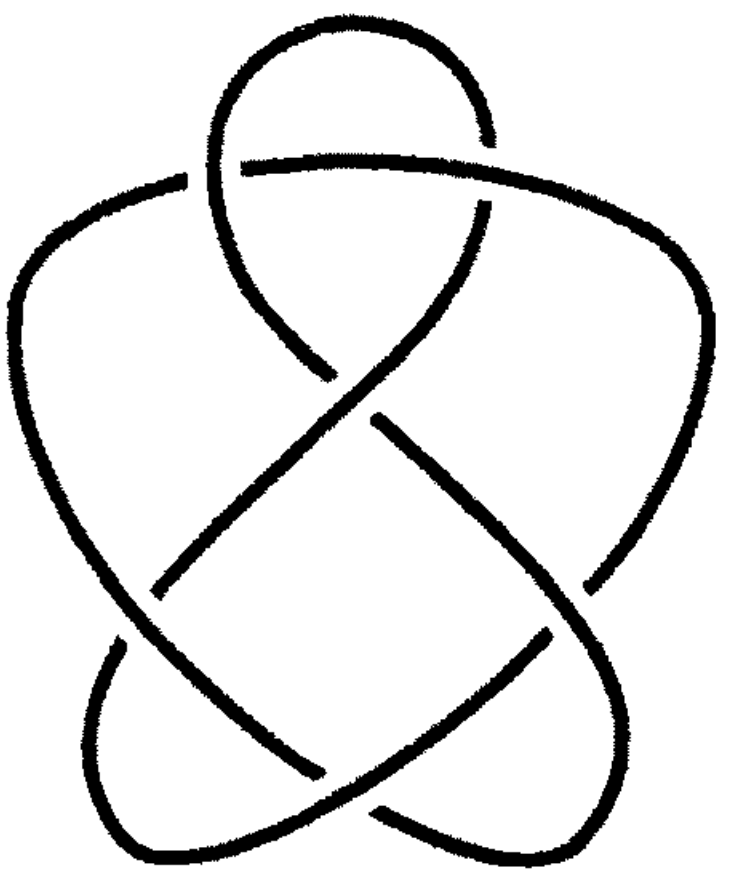
\includegraphics[width=0.8\linewidth]{Blender/ex2-3a.png}
            \caption{$6_2$.}
            \label{fig:ex2-3a}
        \end{subfigure}
        \begin{subfigure}[b]{0.2\linewidth}
            \centering
            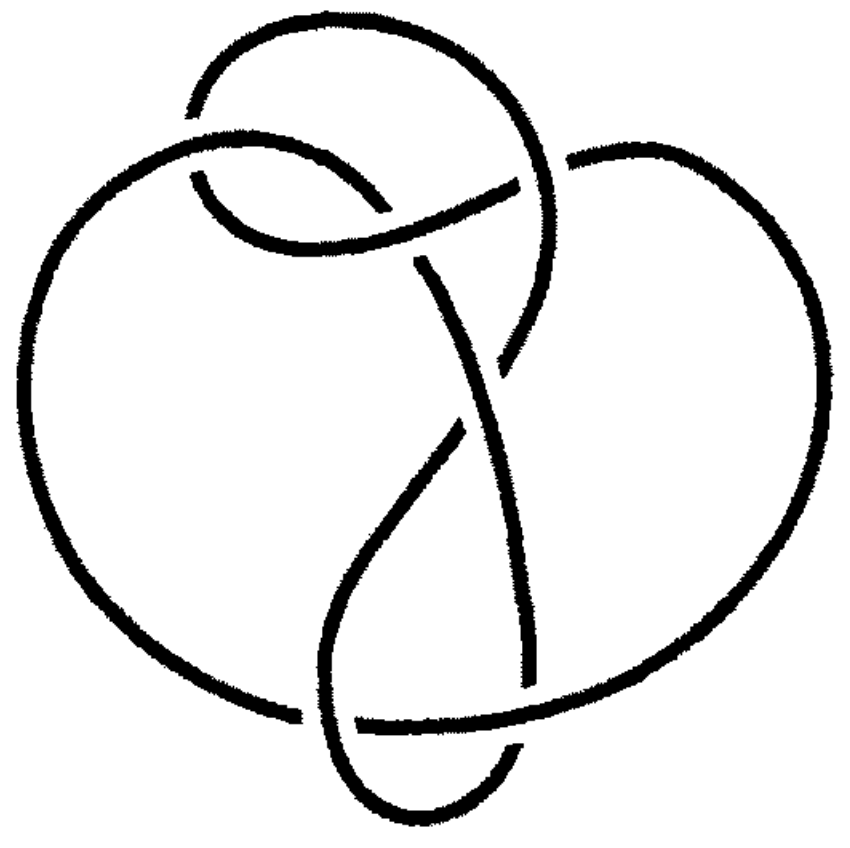
\includegraphics[width=0.7\linewidth]{Blender/ex2-3b.png}
            \caption{$6_3$.}
            \label{fig:ex2-3b}
        \end{subfigure}
        \caption{Knots $6_2$ and $6_3$.}
        \label{fig:ex2-3}
    \end{figure}
    \item Knots can also be reconstructed from Dowker notation. See Figure \ref{fig:reconstruction} for an example of reconstructing an alternating knot from the notation, 8 10 12 2 14 6 4.
    \begin{figure}[h!]
        \centering
        \begin{tikzpicture}[
            every node/.style={black}
        ]
            \begin{knot}[
                clip width=5,
                every strand/.append style={red,thick},
                consider self intersections=true,
                ignore endpoint intersections=false
            ]
                \footnotesize
                \strand[
                    decoration={markings,
                    mark=at position 0.3 with {\arrow{>}},
                    mark=at position 0.9 with {\arrow{>}}},
                    postaction={decorate}
                ] (0,0) to (6,0) to[out=0,in=-90] (7,0.4) to[out=90,in=90,out looseness=0.5] (2,0) node[below left]{2}node[above right]{7} to (2,-0.5);
                \strand (1,0.5) to node[below left]{1}node[above right]{8}  (1,-0.5);
                \strand (3,0.5) to node[below left]{3}node[above right]{10} (3,-0.5);
                \strand (4,0.5) to node[below left]{4}node[above right]{13} (4,-0.5);
                \strand (5,0.5) to node[below left]{5}node[above right]{12} (5,-0.5);
                \strand (6,0.5) to node[below left]{6}node[above right]{11} (6,-0.5);
                \flipcrossings{3,4,6}
                \redraw{1}{(6,0)}
            \end{knot}
        \end{tikzpicture}
        \caption{Constructing a knot projection from its Dowker notation.}
        \label{fig:reconstruction}
    \end{figure}
    \item Our choice in drawing can change the resulting knot.
    \begin{itemize}
        \item 4 6 2 10 12 8 gives two distinct knots.
        \begin{itemize}
            \item \dq{Note that the two knots are composite knots, and that this is refleted in the fact that the sequence 4 6 2 10 12 8 is actually a shuffling of the three numbers 2, 4, 6 and then a shuffling of the three numbers 8, 10, and 12}{38}
        \end{itemize}
        \item When the Dowker notation can be broken into two subpermutations (as above) the knot is composite (unless one subpermutation is trivial).
        \item Any sequence that cannot be split in this way represents either a particular knot or its mirror image.
        \item If the knot is amphicheiral, then the sequence only represent one knot.
    \end{itemize}
    \item A knot and its mirror image are equivalent when projected onto a sphere as opposed to a plane.
    \item \emph{Exercise 2.6}: Draw two projections given by 10 12 2 14 6 4 8, which are inequivalent as projections in the plane but which are equivalent as projections on the sphere.
    \begin{figure}[h!]
        \centering
        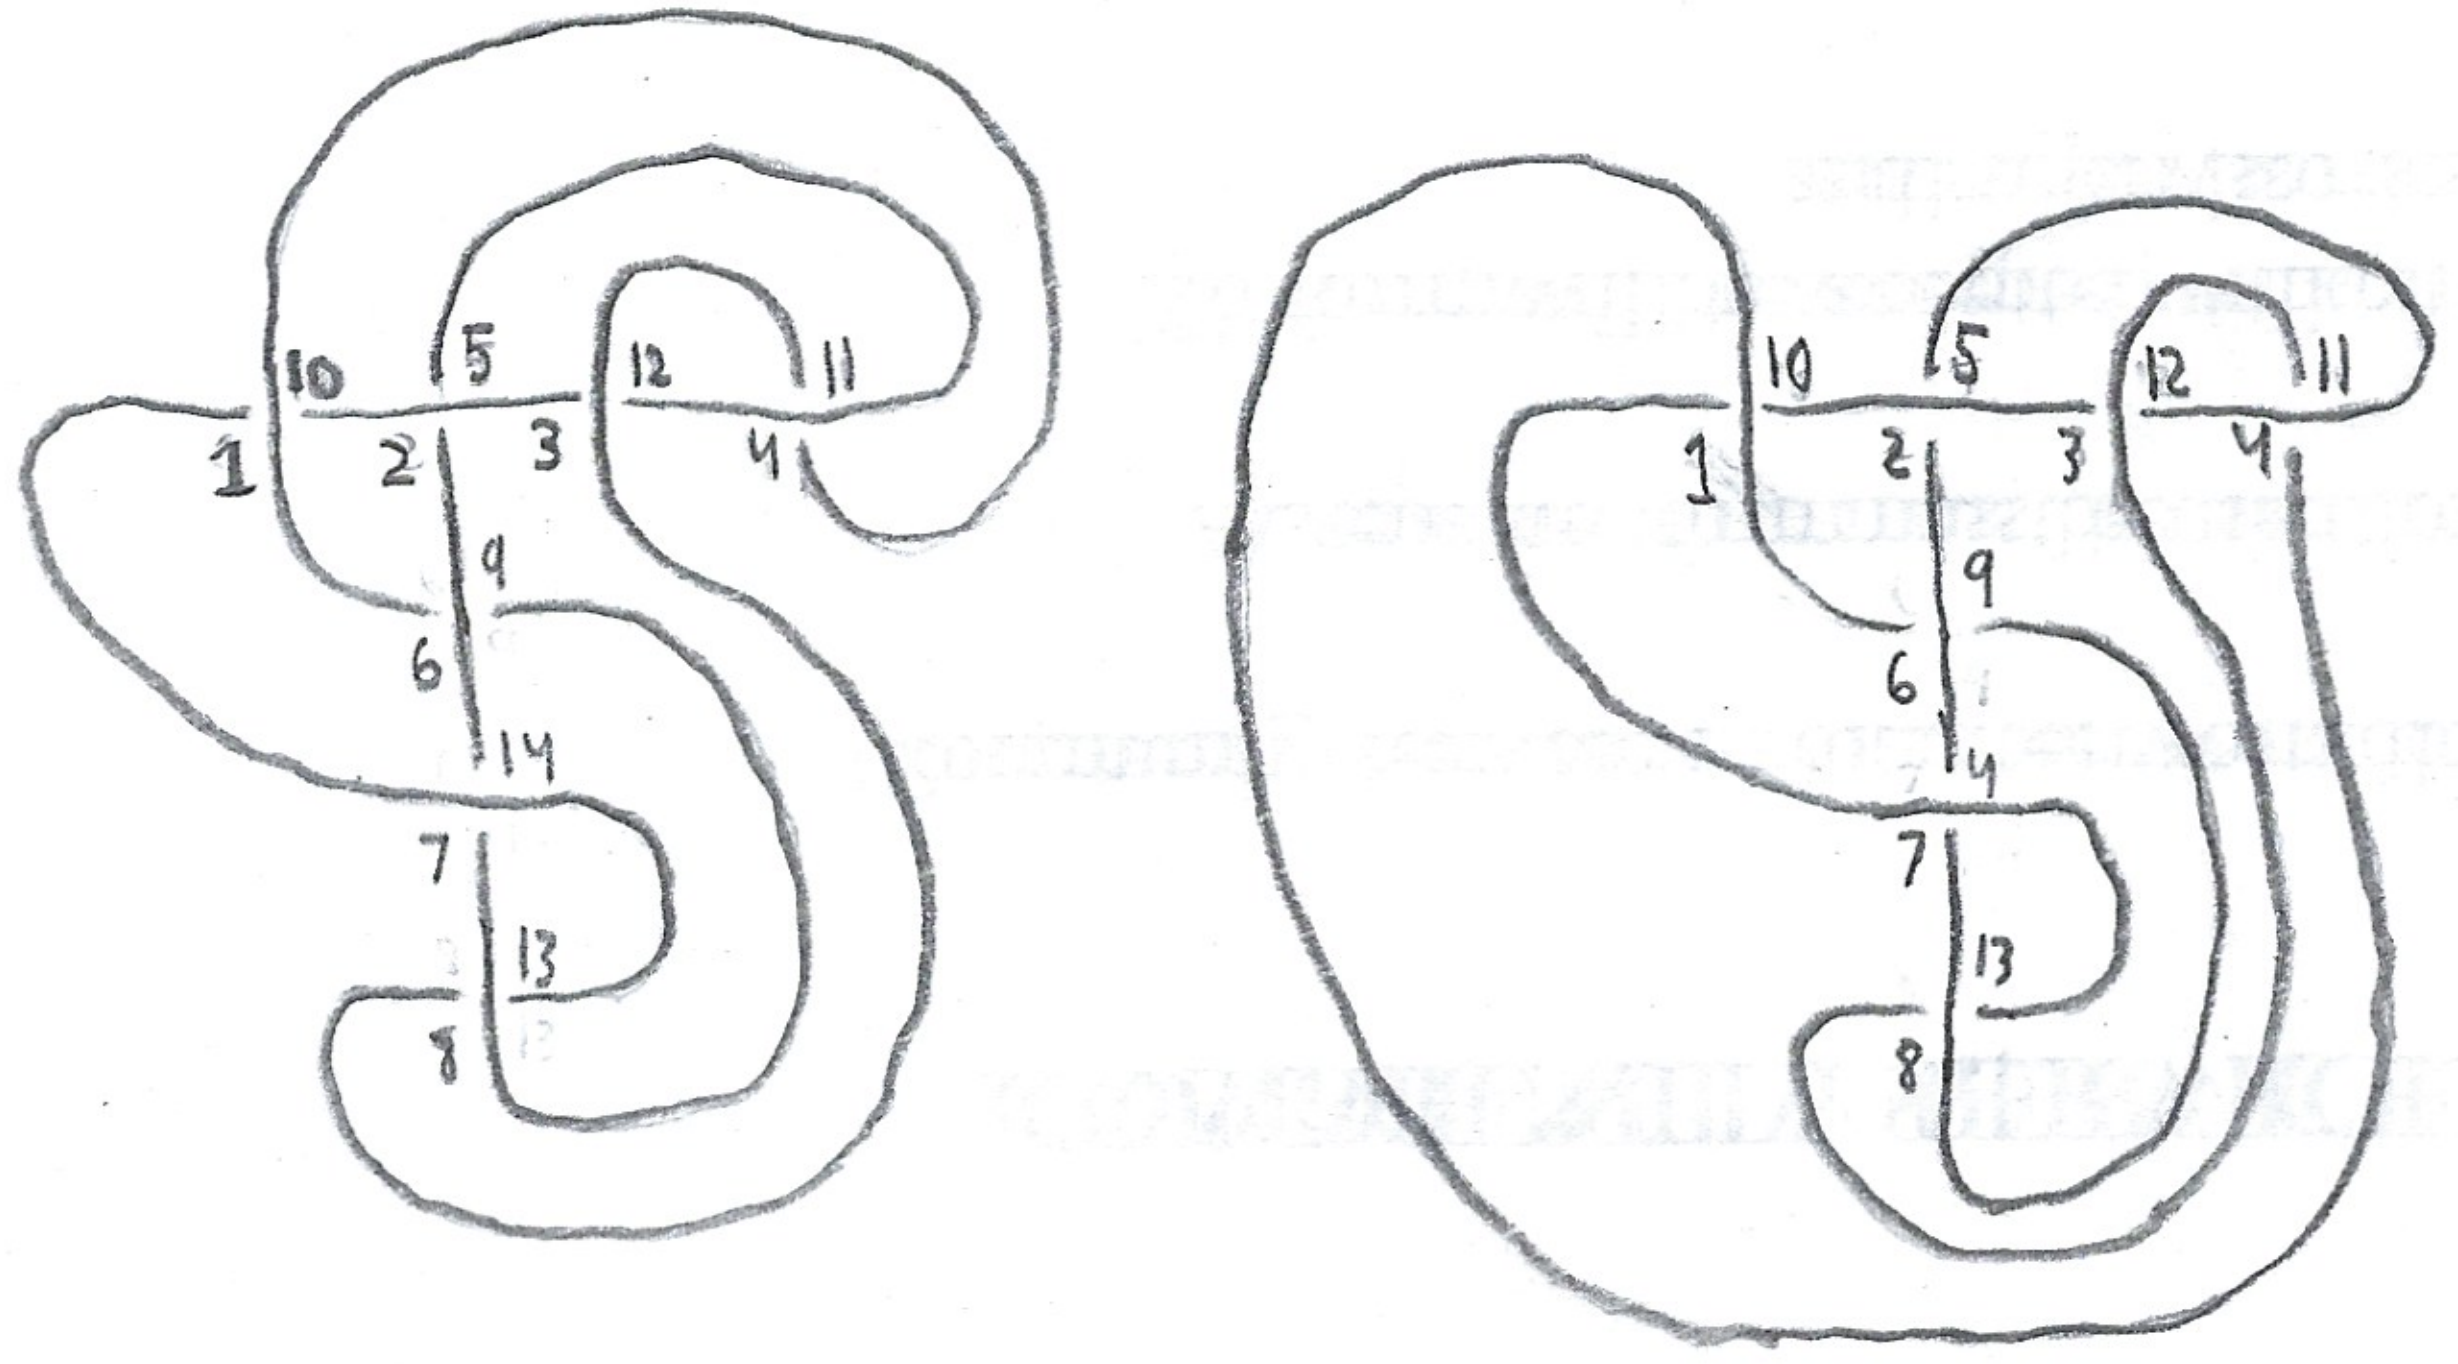
\includegraphics[width=0.5\linewidth]{Blender/ex2-6.png}
        \caption{Solution to \emph{Exercise 2.6}.}
        \label{fig:ex2-6}
    \end{figure}
    \item \emph{Exercise 2.7}: How many different sequences of the integers 2 4 6 8 10 12 14 are there? (This exercise gives us an upper bound on the number of possible alternating knot projections with seven crossings; however, it's far from accurate.)
    \begin{itemize}
        \item There are $7!=5040$ sequences.
    \end{itemize}
    \item There is a slightly modified Dowker notation for nonalternating knots.
    \begin{itemize}
        \item \dq{If the even integer is assigned to the crossing while we are on the overstrand at that crossing, we leave the even integer positive. But if the even integer is assigned to the crossing while we are on the understrand of theat crossing, we make the corresponding even numbers negative}{39}
    \end{itemize}
    \item \emph{Exercise 2.9}: How can you recognize from the sequence of numbers that a projection has a trivial crossing in it like in Figure \ref{fig:ex2-9a}? How about recognizing a Type II Reidemeister move that will reduce the number of crossings by two like in Figure \ref{fig:ex2-9b}?
    \begin{figure}[h!]
        \centering
        \begin{subfigure}[b]{0.3\linewidth}
            \centering
            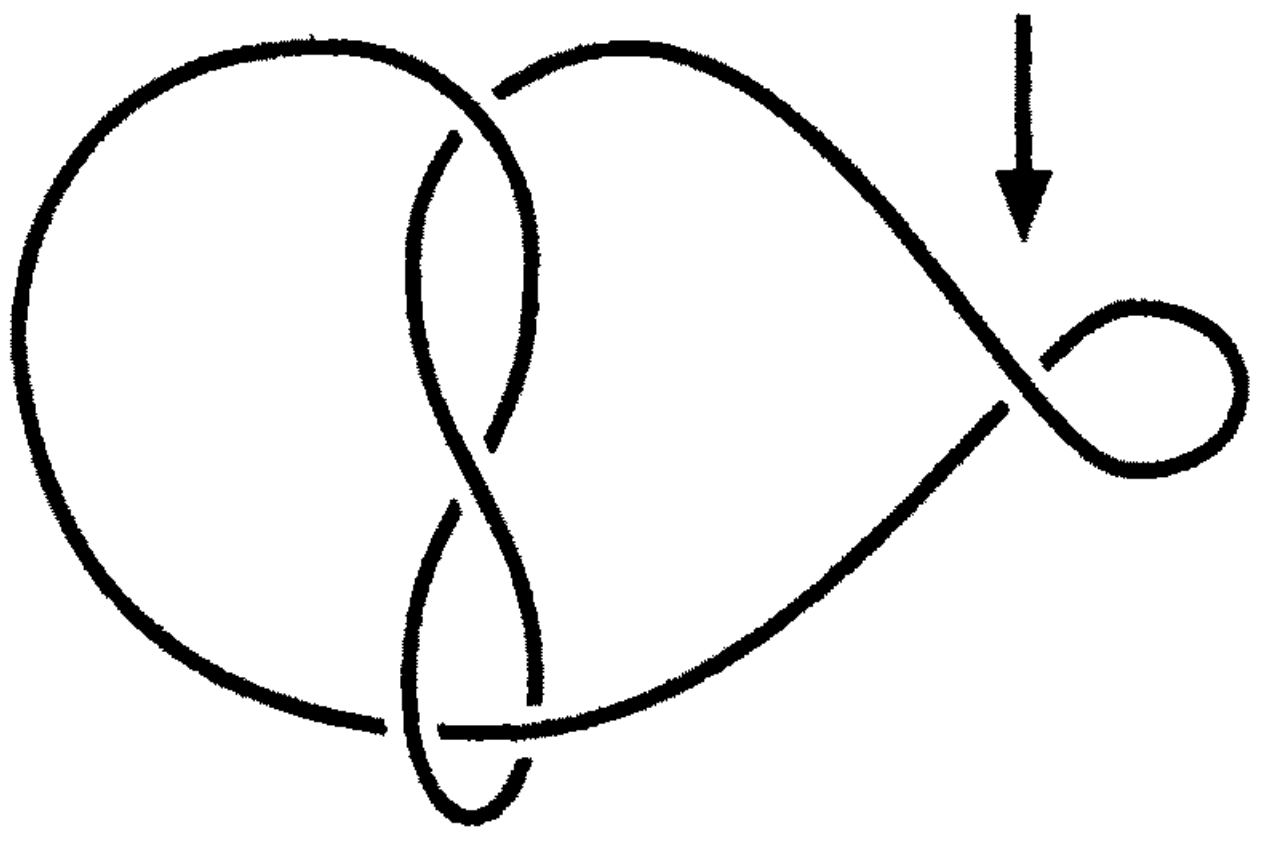
\includegraphics[width=0.6\linewidth]{Blender/ex2-9a.png}
            \caption{Type I Reidemeister move.}
            \label{fig:ex2-9a}
        \end{subfigure}
        \begin{subfigure}[b]{0.3\linewidth}
            \centering
            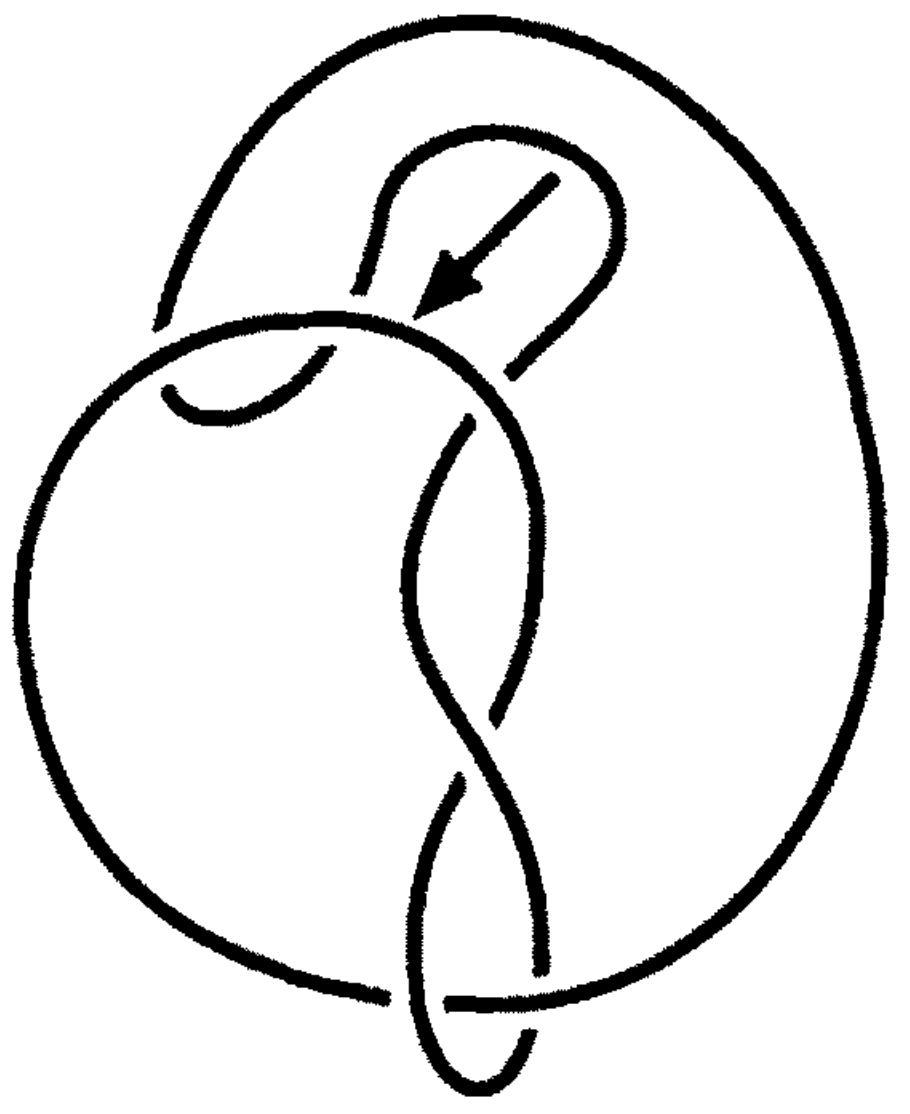
\includegraphics[width=0.53\linewidth]{Blender/ex2-9b.png}
            \caption{Type II Reidemeister move.}
            \label{fig:ex2-9b}
        \end{subfigure}
        \caption{Recognizing extra crossings from the Dowker notation.}
        \label{fig:ex2-9}
    \end{figure}
    \begin{itemize}
        \item A Type I Reidemeister move can be recognized from the Dowker notation sequence by the pairing of two numbers that have an absolute difference of 1. In Figure \ref{fig:ex2-9a}, a sample Dowker notation is 6 2 8 10 4. Since 2 pairs with 3, and $|2-3|=1$, we know that there is a Type I Reidemeister move. Logically, this makes sense because when moving along the orientation, a trivial crossing will be crossed twice in a row.
        \item A Type II Reidemeister move can be recognized from the Dowker notation sequence by a specific characteristic of two pairs: If $(x_1,y_1)$ and $(x_2,y_2)$ is such a pair, where the order is listed such that $|x_2|>|x_1|$ and $|y_1|>|y_2|$, then both of the following must be true.
        \begin{align}
            \big||x_1|-|x_2|\big|=1=\big||y_1|-|y_2|\big| && |x_1-y_2|\neq\big||x_1|-|y_2|\big|\label{eqn:typeIIdowker}
        \end{align}
        In Figure \ref{fig:ex2-9b}, a sample Dowker notation is 8 6 10 $-2$ 12 4. Since ($-2$,7) and (3,6) are pairs that satisfy the above, we know that there is a Type II Reidemeister move. Logically, this makes sense because, when moving along the orientation, such crossings' numbers will be sequential both times crossed (confirmed by the left statement in Equation \ref{eqn:typeIIdowker}). Additionally, the even numbers must have opposite signs or the strand would be linked, as opposed to entirely above or below (confirmed by the right statement in Equation \ref{eqn:typeIIdowker}).
    \end{itemize}
    \item The most consequential fact of Dowker notation is that it allows us to \dq{feed projections of knots into the computer simply as a sequence of numbers}{40}
\end{itemize}


\subsection{Conway's Notation}
\begin{itemize}
    \item Particularly suited to calculations involving \textbf{tangles}.
    \item \textbf{Tangle}: \dq{A region [in a knot or link] in the projection plane surrounded by a circle such that the knot or link crosses the circle exactly four times}{41}
    \begin{itemize}
        \item These four crossings will be thought of as occurring in the four ordinal compass directions.
    \end{itemize}
    \item Tangles can be thought of as building blocks in knot or link projections.
    \item \textbf{Equivalent}: Two tangle projections that can be transformed into each other via a series of Reidemeister moves \dq{while the four endpoints of the strings in the tangle remain fixed and while the strings of the tangle never journey outside the circle defining the tangle}{41}
    \item Notice that, if a knot is formed by gluing together the tangle's ends in pairs, the knot is equivalent to other projections of itself as long as the tangles are equivalent (by a series of Reidemeister moves).
    \item Tangles, such as the one in Figure \ref{fig:tanglesc} are denoted by the number of left-hand twists (crossings).
    \begin{itemize}
        \item If we had twisted the tangle the other way, we would have called it $-3$.
        \item More simply, \dq{for a positive-integer twist, the overstrand always has a positive slope, if we think of it as a small segment of a line [perhaps a cubic, in the case of Figure \ref{fig:tanglesc}]}{42}
    \end{itemize}
    \begin{figure}[h!]
        \centering
        \begin{subfigure}[b]{0.3\linewidth}
            \centering
            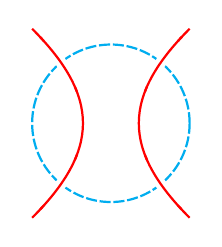
\begin{tikzpicture}
                \begin{knot}[
                    clip width=5
                ]
                    \strand[cyan,thick,only when rendering/.style={dashed,dash pattern={on 4pt off 1pt}}] circle (1cm);
                    \strand[red,thick] (-1,1.2) to[out=-45,in=45,looseness=1.3] (-1,-1.2);
                    \strand[red,thick] (1,1.2) to[out=-135,in=135,looseness=1.3] (1,-1.2);
                    \flipcrossings{1,2,3,4}
                \end{knot}
            \end{tikzpicture}
            \caption{The $\infty$ tangle.}
            \label{fig:tanglesa}
        \end{subfigure}
        \begin{subfigure}[b]{0.3\linewidth}
            \centering
            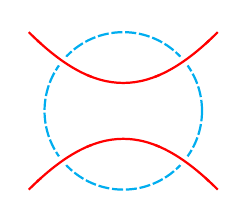
\begin{tikzpicture}
                \begin{knot}[
                    clip width=5
                ]
                    \strand[cyan,thick,only when rendering/.style={dashed,dash pattern={on 4pt off 1pt}}] circle (1cm);
                    \strand[red,thick] (-1.2,1) to[out=-45,in=-135,looseness=1.3] (1.2,1);
                    \strand[red,thick] (-1.2,-1) to[out=45,in=135,looseness=1.3] (1.2,-1);
                    \flipcrossings{1,2,3,4}
                \end{knot}
            \end{tikzpicture}
            \caption{The $0$ tangle.}
            \label{fig:tanglesb}
        \end{subfigure}
        \begin{subfigure}[b]{0.3\linewidth}
            \centering
            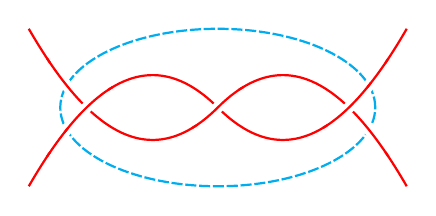
\begin{tikzpicture}
                \begin{knot}[
                    clip width=5,
                    ignore endpoint intersections=false
                ]
                    \strand[cyan,thick,only when rendering/.style={dashed,dash pattern={on 4pt off 1pt}}] ellipse (2cm and 1cm);
                    \strand[red,thick] (-2.4,-1)
                        to[out=60,in=135,looseness=1.3] (0,0)
                        to[out=-45,in=-120,looseness=1.3] (2.4,1)
                    ;
                    \strand[red,thick] (-2.4,1)
                        to[out=-60,in=-135,looseness=1.3] (0,0)
                        to[out=45,in=120,looseness=1.3] (2.4,-1)
                    ;
                    \flipcrossings{1,2,3,4,6}
                \end{knot}
            \end{tikzpicture}
            \caption{The $3$ tangle.}
            \label{fig:tanglesc}
        \end{subfigure}
        \caption{Tangles.}
        \label{fig:tangles}
    \end{figure}
    \item \textbf{0 tangle}: The simplest of all tangles (by definition). \emph{Also known as} \textbf{trivial tangle}. See Figure \ref{fig:tanglesb}.
    \item If we reflect the 3 tangle across a line connecting the NW and SE corners, and then proceed to extrude the NE and SE strands, twisting positively twice, we yield the tangle, 3 2.
    \item If we reflect 3 2 across the same line, and then proceed to extrude the NE and SE stands, twisting negatively four times, we yield the tangle, 3 2 $-4$.
    \item \textbf{Rational tangle}: Any tangle that can be constructed in the manner described in the above 2 bullet points.
    \begin{itemize}
        \item Note that if the tangle is represented by an even number of integers, it can be thought of as being constructed from the $\infty$ tangle, and vice versa for the 0 tangle.
    \end{itemize}
    \item \emph{Exercise 2.10}: Draw the rational tangles corresponding to 2 $-3$ 4 5 and 3 $-1$ 3 $-3$ 2.
    \begin{figure}[H]
        \centering
        \begin{subfigure}[b]{0.4\linewidth}
            \centering
            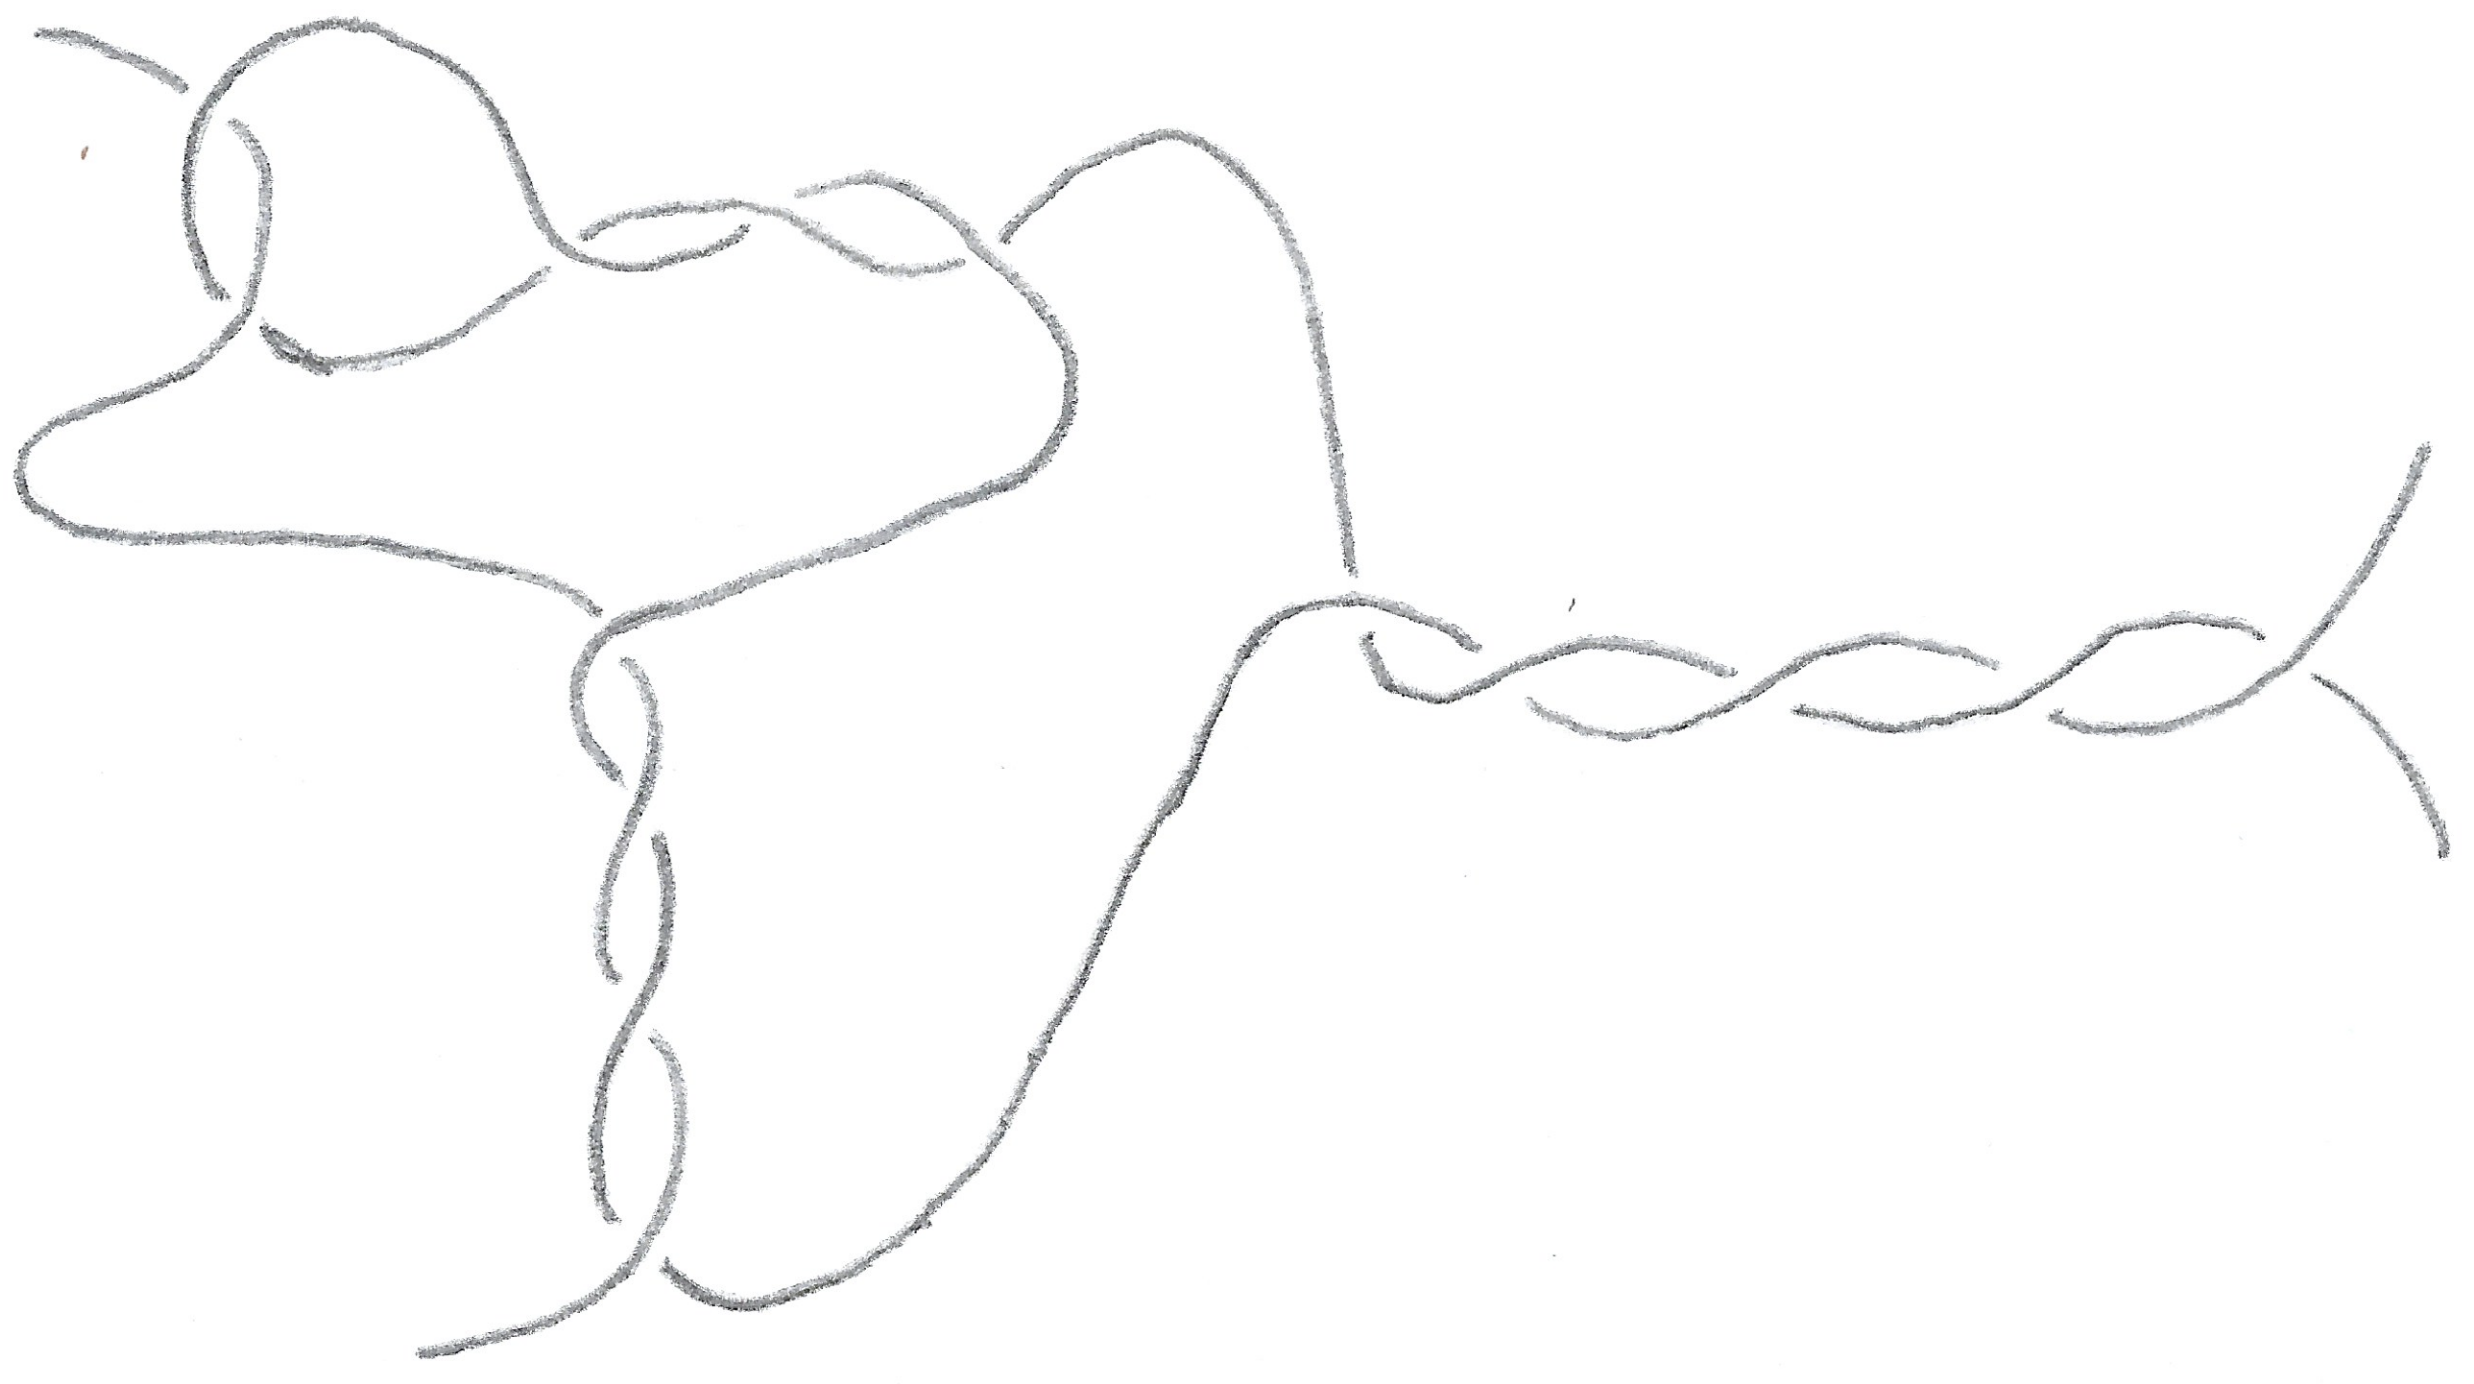
\includegraphics[width=\linewidth]{Blender/ex2-10a.png}
            \caption{The tangle, 2 $-3$ 4 5.}
            \label{fig:ex2-10a}
        \end{subfigure}
        \begin{subfigure}[b]{0.4\linewidth}
            \centering
            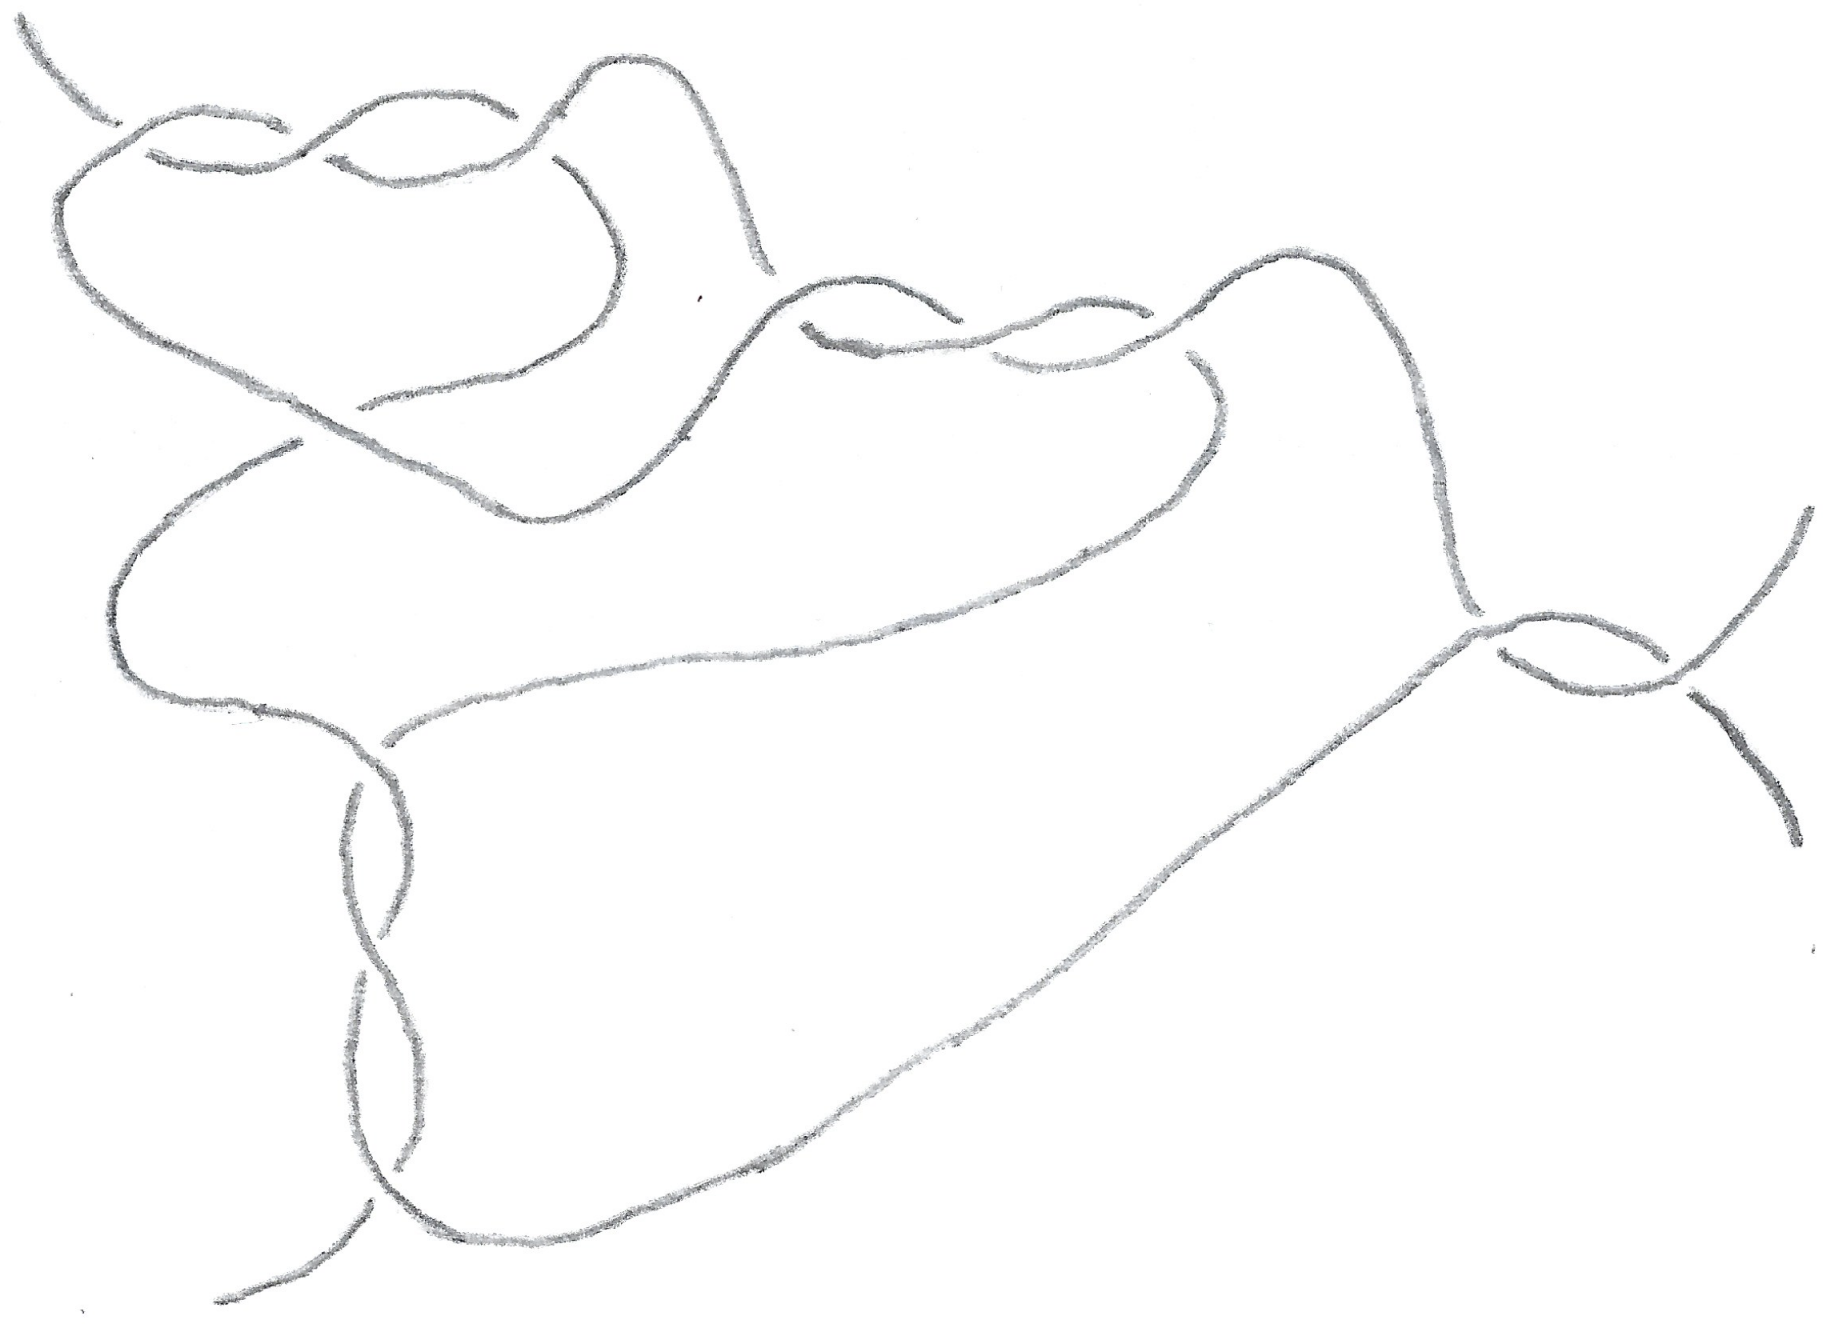
\includegraphics[width=0.8\linewidth]{Blender/ex2-10b.png}
            \caption{The tangle, 3 $-1$ 3 $-3$ 2.}
            \label{fig:ex2-10b}
        \end{subfigure}
        \caption{Solution to \emph{Exercise 2.10}}
        \label{fig:ex2-10}
    \end{figure}
    \item There is an extremely simple way to tell if two rational tangles are equivalent from their notation: \textbf{continued fractions}.
    \item \textbf{Continued fraction}: A fraction obtained through the iterative process of summing a number and its reciprocal.
    \begin{itemize}
        \item For example, given the three numbers a, b, and c, the continued fraction would be the following.
        \begin{equation}
            c+\frac{1}{b+\frac{1}{a}}
        \end{equation}
    \end{itemize}
    \item Applied to knot theory, we know that the tangles, $-2$ 3 2 and 3 $-2$ 3, (seen in Figure \ref{fig:ex2-12}) are equivalent because of the following.
    \begin{align}
        \begin{split}
            2+\frac{1}{3+\frac{1}{-2}} &= 3+\frac{1}{-2+\frac{1}{3}}\\
            2+\frac{1}{\frac{5}{2}} &= 3+\frac{1}{\frac{-5}{3}}\\
            2+\frac{2}{5} &= 3+\frac{-3}{5}\\
            \frac{12}{5} &= \frac{12}{5}\\
        \end{split}
    \end{align}
    \item \emph{Exercise 2.13}: Determine which of the four rational tangles in Figure \ref{fig:ex2-13} are equivalent$^[$\footnote{Idea for first paper: Prove that a series of NE$\leftrightarrow$SE and SE$\leftrightarrow$SW moves is sufficient to generate any rational tangle (like Reidemeister moves). Apply these findings to defining a tangle from a projection. Potentially create a new notation (show how this notation and the current tangle notation convert).}$^]$.
    \begin{figure}[h!]
        \centering
        \begin{subfigure}[b]{0.2\linewidth}
            \centering
            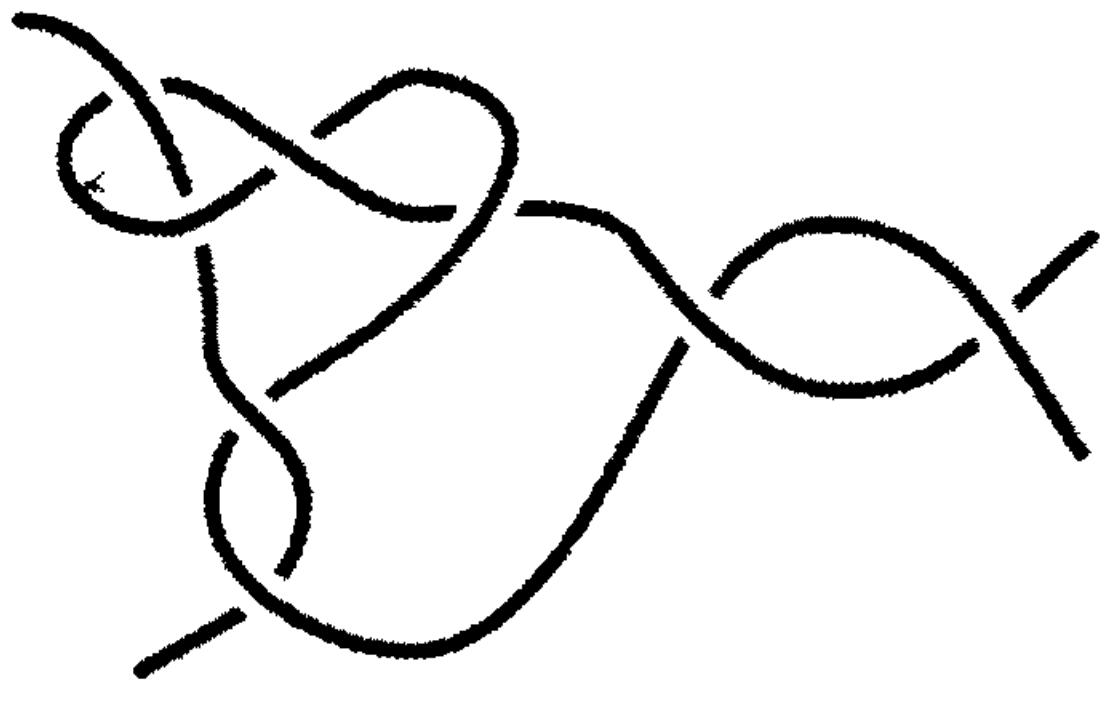
\includegraphics[width=0.8\linewidth]{Blender/ex2-13a.png}
            \caption{Tangle 1.}
            \label{fig:ex2-13a}
        \end{subfigure}
        \begin{subfigure}[b]{0.2\linewidth}
            \centering
            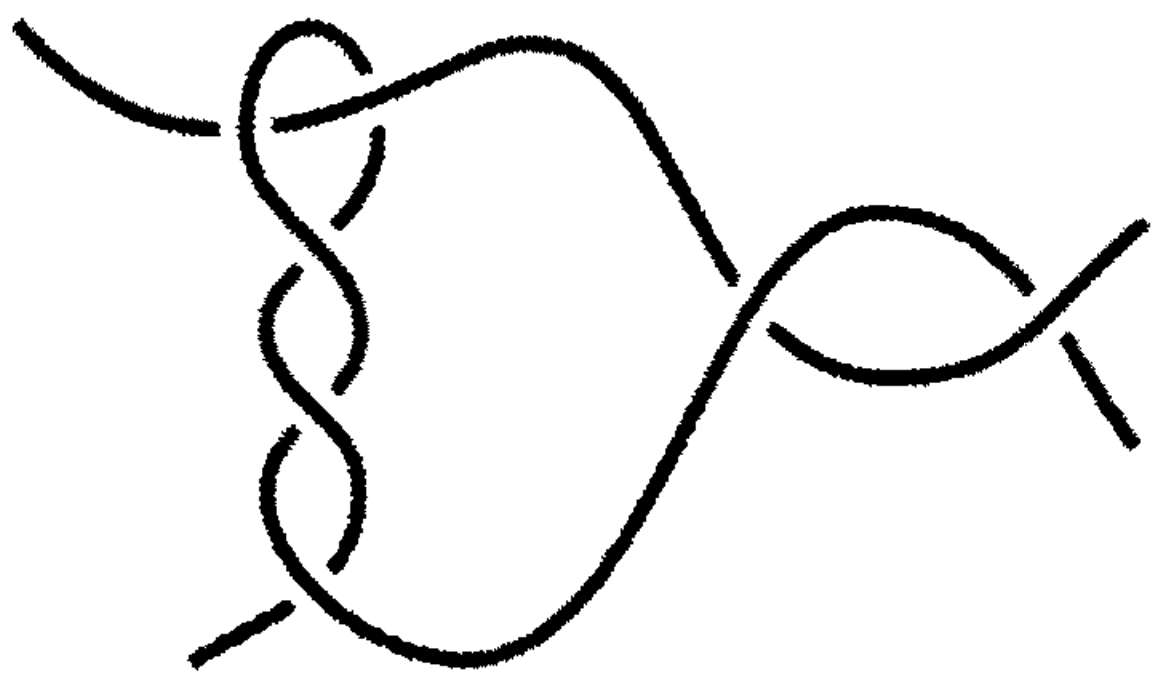
\includegraphics[width=0.8\linewidth]{Blender/ex2-13b.png}
            \caption{Tangle 2.}
            \label{fig:ex2-13b}
        \end{subfigure}
        \begin{subfigure}[b]{0.25\linewidth}
            \centering
            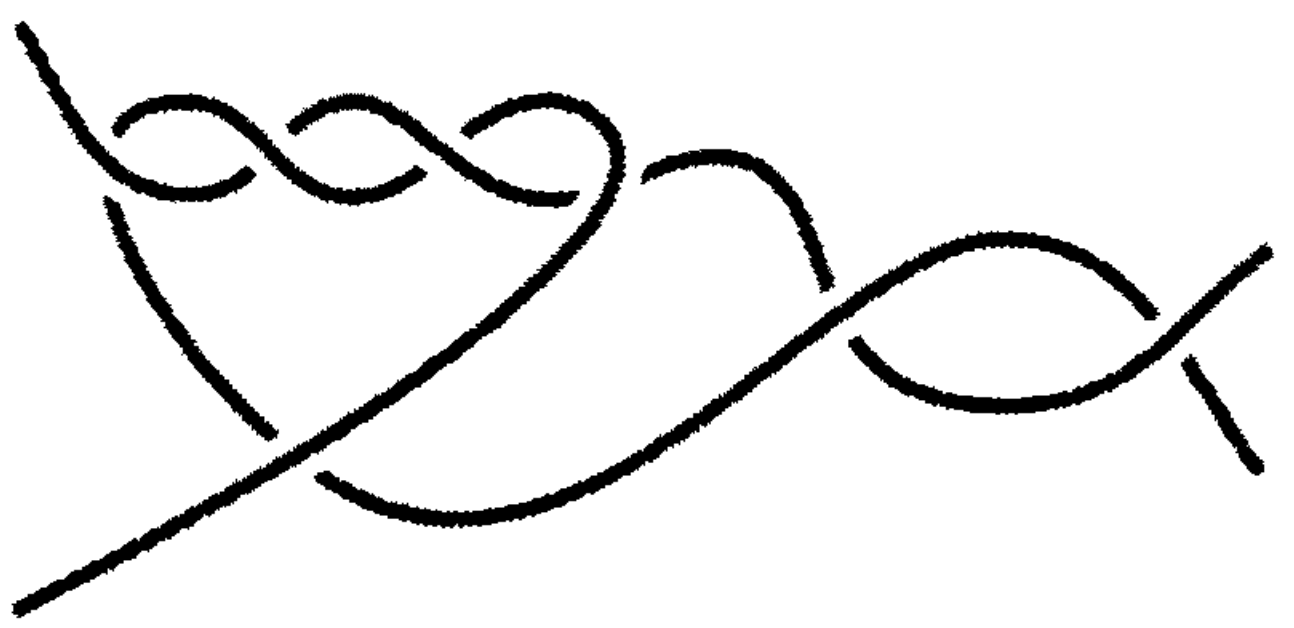
\includegraphics[width=0.8\linewidth]{Blender/ex2-13c.png}
            \caption{Tangle 3.}
            \label{fig:ex2-13c}
        \end{subfigure}
        \begin{subfigure}[b]{0.16\linewidth}
            \centering
            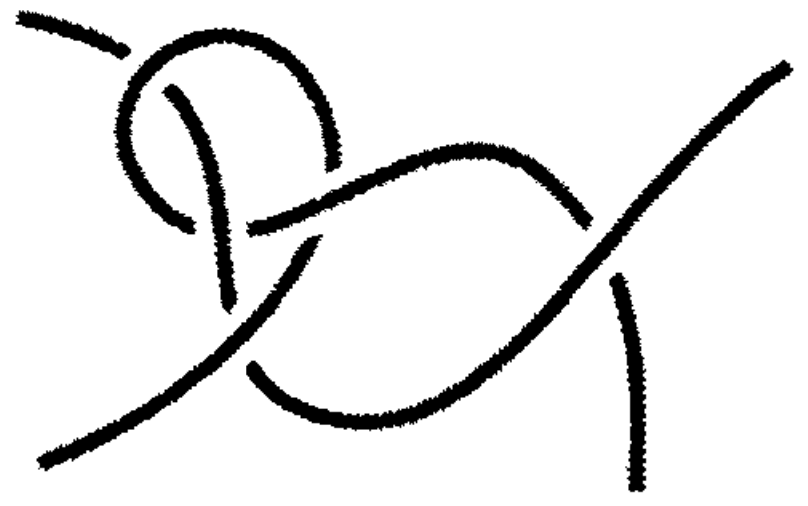
\includegraphics[width=0.8\linewidth]{Blender/ex2-13d.png}
            \caption{Tangle 4.}
            \label{fig:ex2-13d}
        \end{subfigure}
        \caption{Four rational tangles.}
        \label{fig:ex2-13}
    \end{figure}
    \begin{itemize}
        \item Tangle 1 (Figure \ref{fig:ex2-13a}) can be denoted $-1$ $-1$ $-2$ $-2$ $-2$.
        \begin{itemize}
            \item Its continued fraction simplifies as follows.
            \begin{align}
                \begin{split}
                    -2+\frac{1}{-2+\frac{1}{-2+\frac{1}{-1+\frac{1}{-1}}}} &= -2+\frac{1}{-2+\frac{1}{-2+\frac{1}{-2}}}\\
                    &= -2+\frac{1}{-2+\frac{-2}{5}}\\
                    &= -2+\frac{-5}{12}\\
                    &= \frac{-29}{12}\\
                \end{split}
            \end{align}
        \end{itemize}
        \item Tangle 2 (Figure \ref{fig:ex2-13b}) can be denoted 2 $-3$ 2.
        \begin{itemize}
            \item Its continued fraction simplifies as follows.
            \begin{align}
                \begin{split}\label{eqn:ex2-13b}
                    2+\frac{1}{-3+\frac{1}{2}} &= 2+\frac{-2}{5}\\
                    &= \frac{8}{5}\\
                \end{split}
            \end{align}
        \end{itemize}
        \item Tangle 3 (Figure \ref{fig:ex2-13c}) can be denoted $-4$ 1 2.
        \begin{itemize}
            \item Its continued fraction simplifies as follows.
            \begin{align}
                \begin{split}
                    2+\frac{1}{1+\frac{1}{-4}} &= 2+\frac{4}{3}\\
                    &= \frac{10}{3}\\
                \end{split}
            \end{align}
        \end{itemize}
        \item Tangle 4 (Figure \ref{fig:ex2-13d}) can be denoted 1 1 1 1 1.
        \begin{itemize}
            \item Its continued fraction simplifies as follows.
            \begin{align}
                \begin{split}\label{eqn:ex2-13d}
                    1+\frac{1}{1+\frac{1}{1+\frac{1}{1+\frac{1}{1}}}} &= 1+\frac{1}{1+\frac{1}{1+\frac{1}{2}}}\\
                    &= 1+\frac{1}{1+\frac{2}{3}}\\
                    &= 1+\frac{3}{5}\\
                    &= \frac{8}{5}\\
                \end{split}
            \end{align}
        \end{itemize}
        \item Therefore, tangles 2 and 4 (Figures \ref{fig:ex2-13b} and \ref{fig:ex2-13d}, respectively) are equivalent by equations \ref{eqn:ex2-13b} and \ref{eqn:ex2-13d}.
    \end{itemize}
    \item If we close off the ends of a rational tangle, i.e. NE to NW and SE to SW, we form a rational link.
    \item If the link is a knot, we can denote it by its tangle. For example, the figure-eight knot is a rational knot with \textbf{Conway notation} 22 (because of the two twists twice in its center and the gluing of its ends).
    \item \textbf{Conway's notation}: A method of denoting knots by their tangles (all aforementioned theory in this section).
    \item Multiplying tangles:
    \begin{itemize}
        \item Reflect the left tangle across its NW to SE diagonal and then glue its new NE and SE ends to the NW and SW ends, respectively, of the adjacent (to the right) tangle.
        \item Multiplying a rational tangle by an integer tangle will always generate a rational tangle, e.g. 32 comes from multiplying 3 by 2.
        \item To reflect a tangle over its NW-SE line, multiply it by the tangle, 0.
    \end{itemize}
    \begin{figure}[h!]
        \centering
        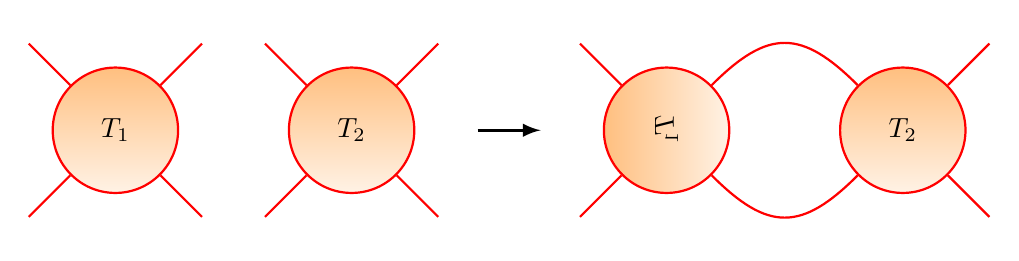
\begin{tikzpicture}
            \node (a) [draw=red,circle,thick,inner sep=4mm] [top color=orange!50,bottom color=orange!10] [xshift=-5cm]                     {$T_1$}
                edge [red,thick] +([xshift=-5cm]1.1,1.1)
                edge [red,thick] +([xshift=-5cm]-1.1,1.1)
                edge [red,thick] +([xshift=-5cm]1.1,-1.1)
                edge [red,thick] +([xshift=-5cm]-1.1,-1.1)
            ;
            \node (b) [draw=red,circle,thick,inner sep=4mm] [top color=orange!50,bottom color=orange!10] [xshift=-2cm]                     {$T_2$}
                edge [red,thick] +([xshift=-2cm]1.1,1.1)
                edge [red,thick] +([xshift=-2cm]-1.1,1.1)
                edge [red,thick] +([xshift=-2cm]1.1,-1.1)
                edge [red,thick] +([xshift=-2cm]-1.1,-1.1)
            ;
            \node (c) [draw=red,circle,thick,inner sep=4mm] [left color=orange!50,right color=orange!10] [rotate=90,xscale=-1,yshift=-2cm] {$T_1$}
                edge [red,thick] +([xshift=2cm]-1.1,1.1)
                edge [red,thick] +([xshift=2cm]-1.1,-1.1)
            ;
            \node (d) [draw=red,circle,thick,inner sep=4mm] [top color=orange!50,bottom color=orange!10] [xshift=5cm]                     {$T_2$}
                edge [red,thick] +([xshift=5cm]1.1,1.1)
                edge [red,thick] +([xshift=5cm]1.1,-1.1)
                edge [red,thick,bend left=45,looseness=1.4]  (c)
                edge [red,thick,bend left=-45,looseness=1.4] (c)
            ;
    
            \draw[very thick,-latex] (-0.4,0) -- (0.4,0);
        \end{tikzpicture}
        \caption{Multiplying tangles.}
        \label{fig:tanglemultiply}
    \end{figure}
    \item Adding tangles:
    \begin{itemize}
        \item Glue the left tangle's NE and SE ends to the right tangle's NW and SW ends, respectively.
        \item Note that no reflecting occurs here.
        \item \dq{If we multiply each tangle in a sequence of tangles by 0, and then add them all together, we denote the resultant tangle by the sequence of numbers that stand for the original tangles, only now separated by commas}{48}
    \end{itemize}
    \item \textbf{Pretzel knot}: \dq{A knot obtained from a tangle represented by a finite number of integers separated by commas}{48}
    \item \textbf{Algebraic tangle}: \dq{Any tangle obtained by the operations of addition and multiplication on rational tangles}{48}
    \item \textbf{Algebraic link}: \dq{A link formed when we connect the NW string to the NE string and the SW string to the SE string on an algebraic tangle}{48} \emph{Also known as} \textbf{aborescent link}.
    \begin{itemize}
        \item Denoted the same way as a tangle.
        \item Fun fact: The trefoil knot (Figure \ref{fig:circletrefoilb}) is an algebraic link of the 3 tangle (Figure \ref{fig:tanglesc}).
    \end{itemize}
    \item \textbf{Additive identity}: A quantity that can be added to a second quantity without changing that second quantity.
    \begin{itemize}
        \item 0 is an additive identity for the real numbers.
    \end{itemize}
    \item \emph{Exercise 2.21}: Is there an additive identity for tangles?
    \begin{itemize}
        \item The 0 tangle (Figure \ref{fig:tanglesb}) is an additive identity for tangles. Adding the 0 tangle does the same thing as extruding (performing a planar isotropy on) the NE and SE strands. Such an addition does not change the relative position of any strand's ordinal end(s).
        \item Continuing the analogy to the real numbers, it makes sense that the 0 tangle would be analogous to 0, the real number.
    \end{itemize}
    \item \textbf{Multiplicative identity}: A quantity that can be multiplied by a second quantity without changing that second quantity.
    \begin{itemize}
        \item 1 is a multiplicative identity for the real numbers.
    \end{itemize}
    \item \emph{Exercise 2.22}: Is there a multiplicative identity for tangles? Is it the same if you multiply a tangle by it on the right side or the left side?
    \begin{itemize}
        \item The 0 tangle (Figure \ref{fig:tanglesb}) is a multiplicative identity for tangles. Multiplying the 0 tangle does the same thing as extruding (performing a planar isotropy on) the SE and SW strands. Such a multiplication does not change the relative position of any strand's ordinal end(s).
        \item To part 2, yes.
    \end{itemize}
    \item The analogy to real numbers does not hold in some areas.
    \begin{itemize}
        \item Multiplication on tangles is not commutative --- $ab\neq ba$ for tangles.
        \item Multiplication on tangles is not associative --- $(ab)c\neq a(bc)$ for tangles.
        \item There are no inverse tangles --- there is no tangle that when added to $T$ gives back the trivial tangle, 0.
    \end{itemize}
    \item There are tangles that are not algebraic.
    \item New knots can be obtained via \textbf{mutation}.
    \item \textbf{Mutation}: Severing the connections between a tangle and any adjacent tangles, transforming it (flipping horizontally, vertically, or both), and gluing the strands to their new adjacent counterparts.
    \begin{itemize}
        \item Knots formed in this manner are called \textbf{mutants} of one another.
    \end{itemize}
    \item \emph{Exercise 2.25}: Show that if we have three tangles as in Figure \ref{fig:ex2-25a}, we can mutate several times in order to permute the tangles. Note that we can then permute $n$ tangles in a row.
    \begin{figure}[h!]
        \centering
        \begin{subfigure}[b]{0.4\linewidth}
            \centering
            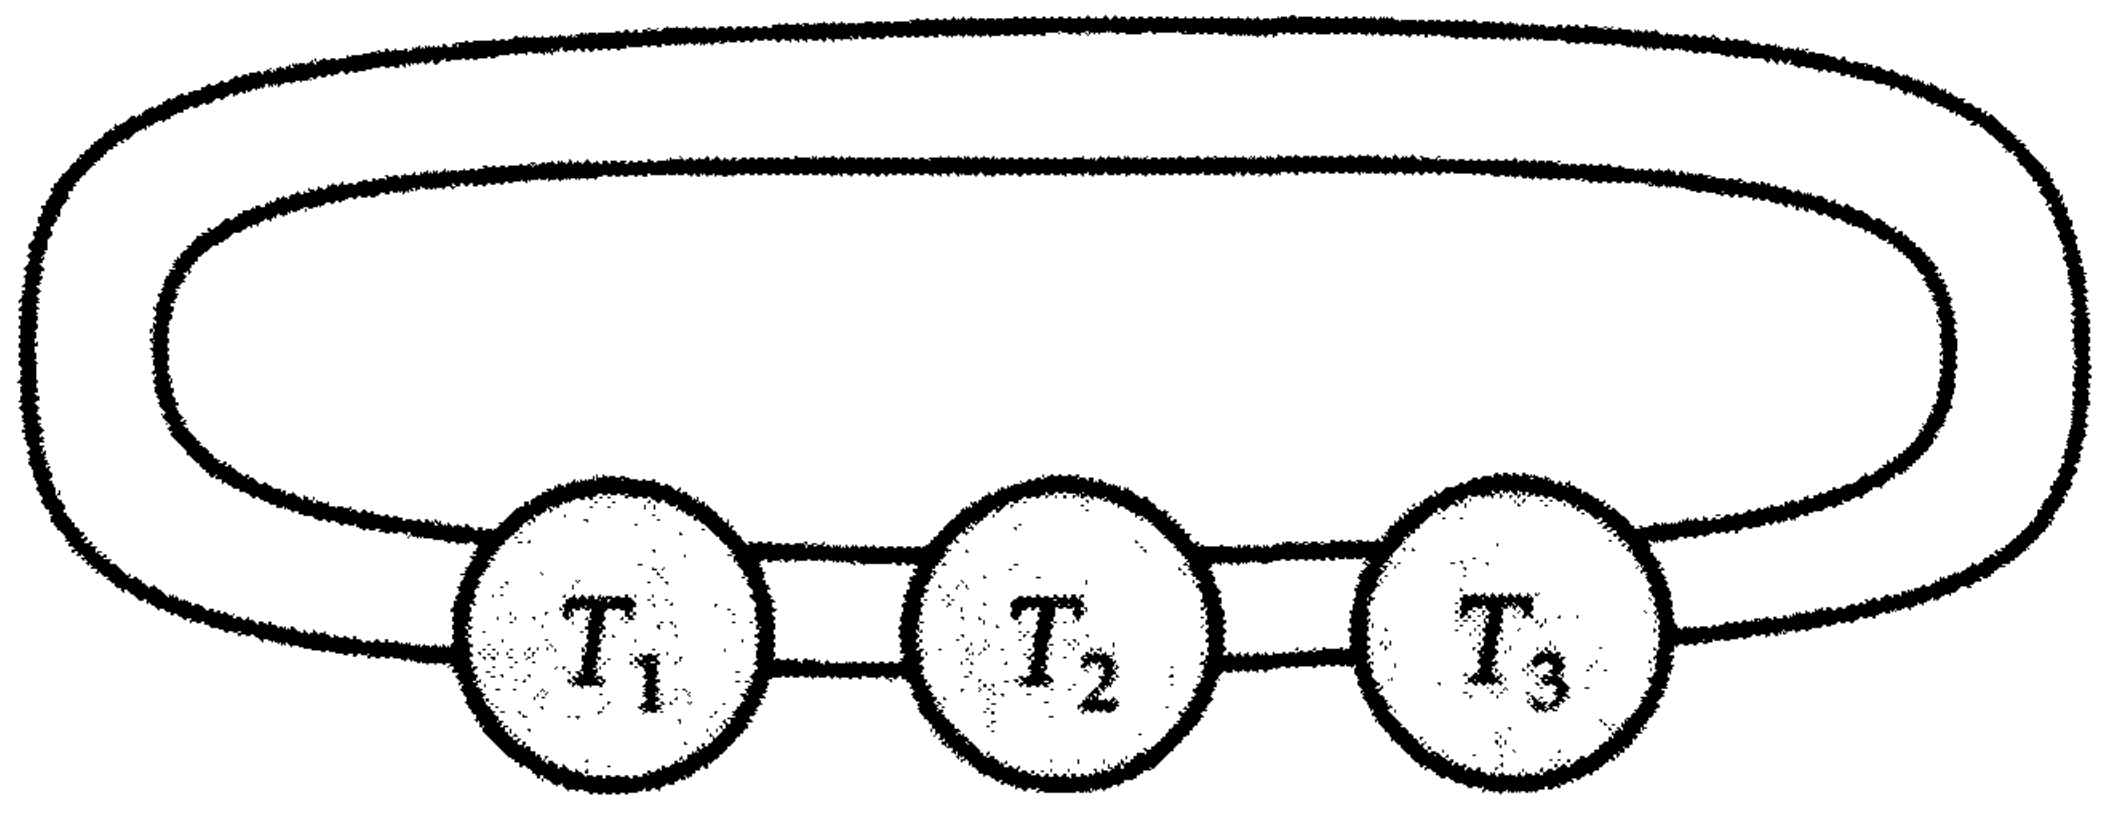
\includegraphics[width=0.8\linewidth]{Blender/ex2-25a.png}
            \caption{A knot.}
            \label{fig:ex2-25a}
        \end{subfigure}
        \begin{subfigure}[b]{0.4\linewidth}
            \centering
            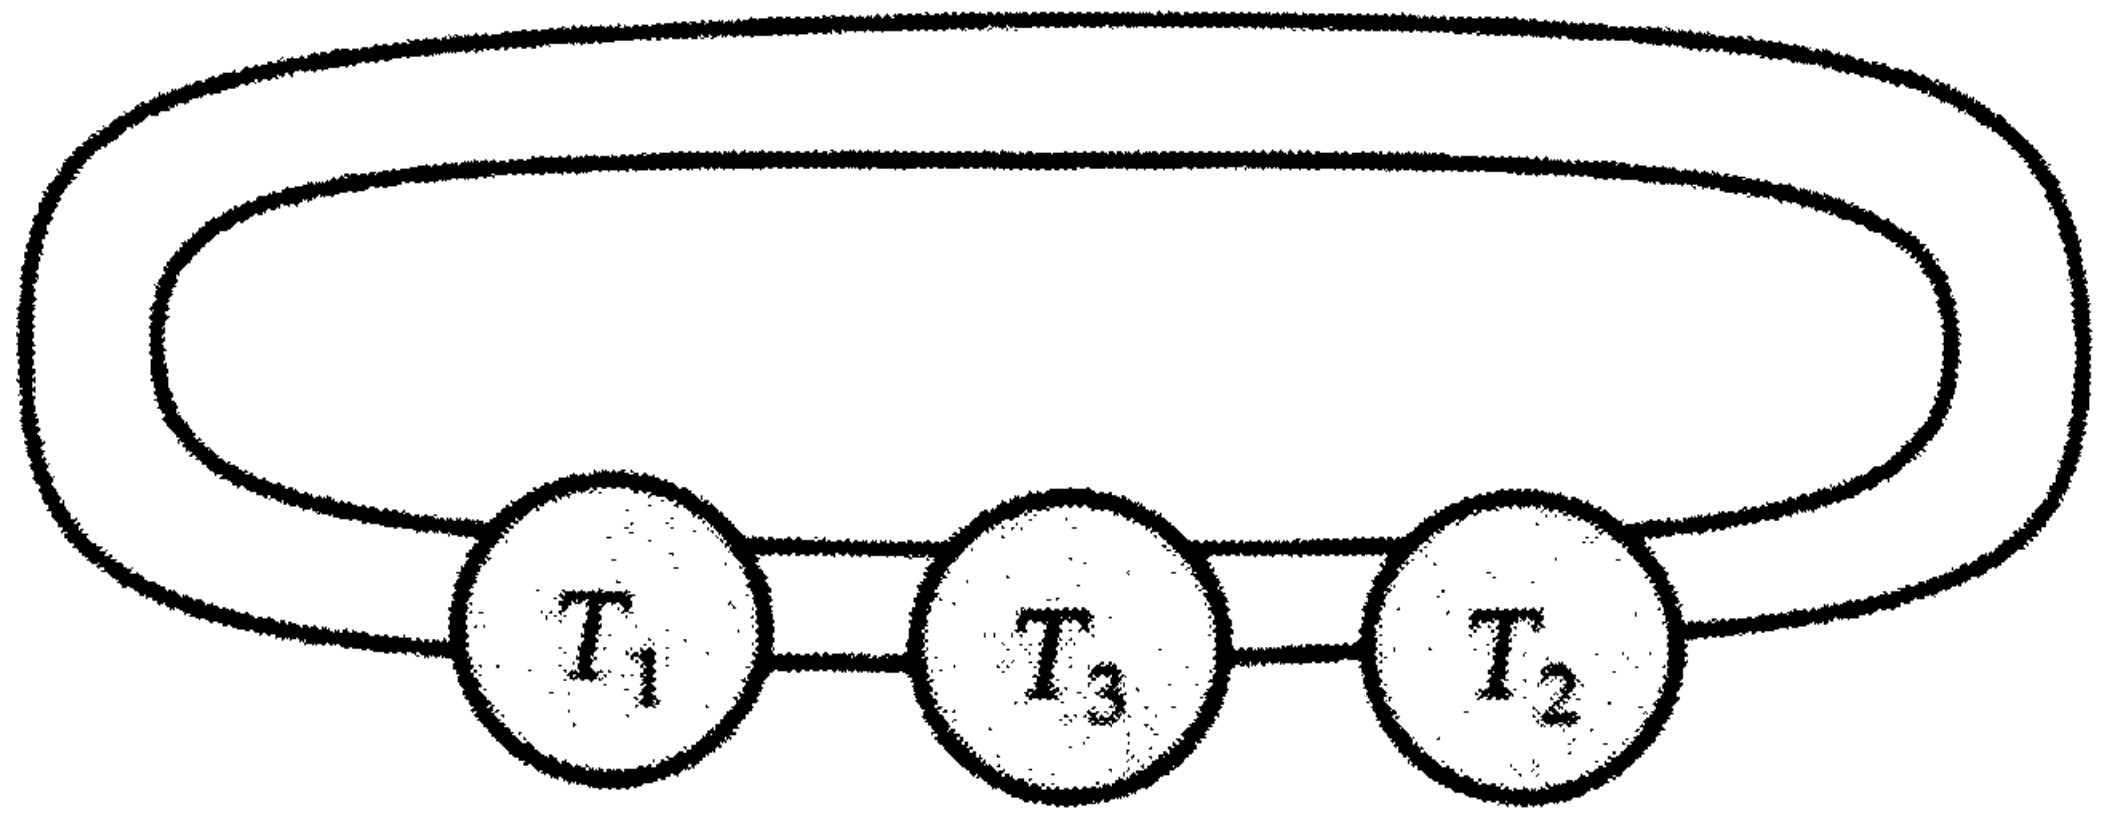
\includegraphics[width=0.8\linewidth]{Blender/ex2-25b.png}
            \caption{A mutant.}
            \label{fig:ex2-25b}
        \end{subfigure}
        \caption{Series of mutations.}
        \label{fig:ex2-9}
    \end{figure}
    \begin{itemize}
        \item Beginning in Figure \ref{fig:ex2-25a}, horizontally flip $T_2$.
        \item Horizontally flip $T_3$.
        \item Horizontally flip the unit of the flipped $T_2$ and $T_3$.
    \end{itemize}
    \item Mutation cannot turn a nontrivial knot into the trivial knot (Figure \ref{fig:circletrefoila}).
    \item More on mutant knots can be found in Sections \ref{sse:polynomials} and \ref{sse:biochemphys}.
\end{itemize}


\subsection{Knots and Planar Graphs}
\begin{itemize}
    \item This section's notation bridges knot theory and graph theory.
    \begin{itemize}
        \item It is capable of contributing to both branches of mathematics.
    \end{itemize}
    \item \textbf{Graph}: A set of points called vertices that are connected by edges.
    \item \textbf{Planar graph}: A graph that lies in a plane.
    \item Creating a planar graph from a projection of a knot or link:
    \begin{itemize}
        \item \dq{Shade every other region of the link projection so that the infinite outermost region is not shaded}{51}
        \item \dq{Put a vertex at the center of each shaded region and then connect with an edge any two vertices that are in regions that share a crossing}{52}
        \item Assign an orientation.
        \item \dq{Label each edge in the planar graph with a $+$ or a $-$, depending on whether the edge passes through a $+$ crossing or a $-$ crossing}{52} See Figure \ref{fig:crossingsign}. Recall computing link numbers in Section \ref{sss:Links} (see Figure \ref{fig:linkingnumber}, specifically).
        \item The result is a \textbf{signed planar graph}. See Figure \ref{fig:graphtrefoil} for an original example.
    \end{itemize}
    \begin{figure}[h!]
        \centering
        \begin{subfigure}[b]{0.2\linewidth}
            \centering
            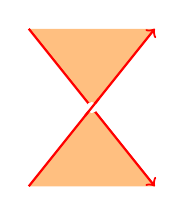
\begin{tikzpicture}
                \fill[orange!50] (-0.8,1) -- (0,0) -- (0.8,1);
                \fill[orange!50] (-0.8,-1) -- (0,0) -- (0.8,-1);
                \begin{knot}[
                    clip width=5,
                    clip radius=2pt,
                    every strand/.append style={red,thick,->}
                ]
                    \strand (-0.8,-1) to (0.8,1);
                    \strand (-0.8,1) to (0.8,-1);
                \end{knot}
            \end{tikzpicture}
            \caption{Denote $+$.}
            \label{fig:crossingsigna}
        \end{subfigure}
        \begin{subfigure}[b]{0.2\linewidth}
            \centering
            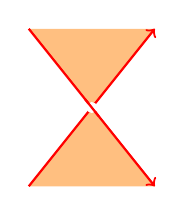
\begin{tikzpicture}
                \fill[orange!50] (-0.8,1) -- (0,0) -- (0.8,1);
                \fill[orange!50] (-0.8,-1) -- (0,0) -- (0.8,-1);
                \begin{knot}[
                    clip width=5,
                    clip radius=2pt,
                    every strand/.append style={red,thick,->},
                    flip crossing=1
                ]
                    \strand (-0.8,-1) to (0.8,1);
                    \strand (-0.8,1) to (0.8,-1);
                \end{knot}
            \end{tikzpicture}
            \caption{Denote $-$.}
            \label{fig:crossingsignb}
        \end{subfigure}
        \caption{Computing signs per crossing.}
        \label{fig:crossingsign}
    \end{figure}
    \begin{figure}[h!]
        \centering
        \begin{subfigure}[b]{0.3\linewidth}
            \centering
            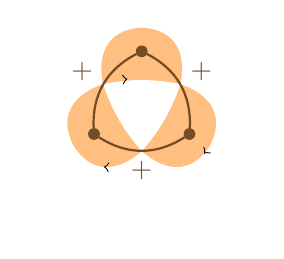
\begin{tikzpicture}
                \fill [orange!50] (90:1)
                    \foreach \x in {1,2,3} {
                        to [bend left=117,looseness=1.9] ({90+120*\x}:1)
                    }
                ;
                \fill [white] (30:0.57)
                    \foreach \x in {1,2,3} {
                        to [bend left=10] ({30-120*\x}:0.57)
                    }
                ;
    
                \begin{knot}[
                    clip width=5,
                    clip radius=2pt,
                    every strand/.append style={red,thick},
                    consider self intersections
                ]
                    \strand [
                        decoration={markings,
                        mark=at position 0.28 with {\arrow{>}},
                        mark=at position 0.48 with {\arrow{>}},
                        mark=at position 0.68 with {\arrow{>}}},
                        postaction={decorate}
                    ] (90:1)
                        \foreach \x in {1,2,3} {
                            to [bend left=117,looseness=1.9] ({90+120*\x}:1)
                        }
                    ;
                    \flipcrossings{1,3}
                \end{knot}
    
                \node (a) [circle,line width=0pt,fill=brown!60!black,inner sep=1.5pt] at (90:0.7){};
                \node (b) [circle,line width=0pt,fill=brown!60!black,inner sep=1.5pt] at (-30:0.7){}
                    edge [brown!60!black,thick,bend right=33] node[anchor=-150]{$+$} (a)
                ;
                \node (c) [circle,line width=0pt,fill=brown!60!black,inner sep=1.5pt] at (-150:0.7){}
                    edge [brown!60!black,thick,bend right=33] node[anchor=north]{$+$} (b)
                    edge [brown!60!black,thick,bend left=33]  node[anchor=-30]  {$+$} (a)
                ;
            \end{tikzpicture}
            \vspace{-0.7cm}
            \caption{Shaded trefoil projection.}
            \label{fig:graphtrefoila}
        \end{subfigure}
        \begin{subfigure}[b]{0.3\linewidth}
            \centering
            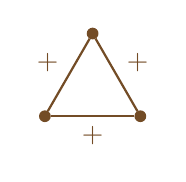
\begin{tikzpicture}
                \node (a) [circle,line width=0pt,fill=brown!60!black,inner sep=1.5pt] at (90:0.7){};
                \node (b) [circle,line width=0pt,fill=brown!60!black,inner sep=1.5pt] at (-30:0.7){}
                    edge [brown!60!black,thick] node[anchor=-150]{$+$} (a)
                ;
                \node (c) [circle,line width=0pt,fill=brown!60!black,inner sep=1.5pt] at (-150:0.7){}
                    edge [brown!60!black,thick] node[anchor=north]{$+$} (b)
                    edge [brown!60!black,thick] node[anchor=-30]  {$+$} (a)
                ;
            \end{tikzpicture}
            \vspace{-0.2cm}
            \caption{Signed planar graph.}
            \label{fig:graphtrefoilb}
        \end{subfigure}
        \caption{A signed planar graph from the standard trefoil knot projection.}
        \label{fig:graphtrefoil}
    \end{figure}
    \item It is also possible return the signed planar graph to a knot projection:
    \begin{itemize}
        \item \dq{Put an $x$ across each edge}{53}
        \item \dq{Connect the edges inside each region of the graph}{53}
        \item \dq{Shade those areas that contain a vertex}{53}
        \item \dq{At each of the $x$'s, put in a crossing corresponding to whether the edge is a $+$ edge or a $-$ edge}{53}
    \end{itemize}
    \item The significance here, as previously referenced, is that we can turn questions about knots into questions about graphs.
    \item \emph{Exercise 2.31}: What do the Reidemeister moves become when translated into operations on signed planar graphs? (Make sure you consider what happens when different regions are shaded.)
    \begin{itemize}
        \item Type I Reidemeister move: Extend an edge from one vertex to a newly created one. Either sign is acceptable (the sign option is analogous to the over-under crossing option).
        \item Type II Reidemeister move: Add two edges connecting two, specific vertices and intersecting no other edges. The signs on the new edges must be opposite, but it either can be positive (or negative; this option is analogous to the over-under crossing option).
        \item Type III Reidemeister move: I do not know$^[$\footnote{Return to this later.}$^]$.
    \end{itemize}
    \item See Section \ref{sss:StatisticalMechanics} for more on signed planar graphs.
\end{itemize}
\newpage



\section{Invariants of Knots}
\subsection{Unknotting Number}\label{sss:UnknottingNumber}
\begin{itemize}
    \item \textbf{Unknotting number}: A value $n\in\mathbb{N}$ specific to a knot $K$ that gives the fewest number of crossing changes needed in any projection to turn it into the unknot. \emph{Also known as} $\mathbf{u(K)}$.
    \begin{itemize}
        \item It may, however, be a nasty projection of the unknot (see Figure \ref{fig:ex1-11-2} and the related Exercise).
    \end{itemize}
    \item \emph{Exercise 3.1}: Find the unknotting number of the figure-eight knot (Figure \ref{fig:figure8knot}).
    \begin{itemize}
        \item $u(K)=1$, where $K$ is the figure-eight knot.
        \item $K$ is distinct from the unknot, so $u(K)\neq 0$. The next possibility ($u(K)=1$) succeeds with the projection in Figure \ref{fig:figure8knot} (in fact, flipping \emph{any} crossing in the referenced projection trivializes $K$).
    \end{itemize}
    \item Note that performing all of the crossing changes on one projection is equivalent to performing one such change, then an ambient isotropy, then another\dots
    \begin{itemize}
        \item A proof of this is listed on page 58.
    \end{itemize}
    \item \dq{The fact that every knot has a finite unknotting number follows from the fact that every projection of a knot can be changed into a projection of the unknot by changing some subset of the crossings in the projection}{58}
    \begin{itemize}
        \item See Exercise 1.7.
    \end{itemize}
    \item A proof of the above:
    \begin{itemize}
        \item Pick a starting point (not a crossing) on an arbitrary knot and an orientation in whose direction to traverse the knot.
        \item When you arrive at the first crossing, change it so that the strand that you are on is the over strand, if necessary.
        \item Continue changing every new crossing to which you come to make the current strand into the overstrand.
        \begin{itemize}
            \item Do not change crossings that you have already passed through once.
        \end{itemize}
        \item At this point, you now have a projection of a knot that was obtained from the original knot by changing crossings and that is the trivial knot. A proof of this triviality follows.
        \medskip
        \item Consider the knot in three-space, with the $z$-axis coming out of the page. Assign to the starting point the $z$-coordinate, $z=1$.
        \item Decrease the $z$-coordinate of each consecutive point as you traverse the knot, culminating in the original point being labeled, $z=0$.
        \begin{itemize}
            \item Connect the starting and ending points with a vertical bar to preserve the knot as a knot.
        \end{itemize}
        \item What you have now obtained is a knot in three-space that, when projected from the top is the knot that we constructed before the line break, but has no crossings when projected from the side (and is therefore the trivial knot).
        \item Q.E.D.
    \end{itemize}
    \item It is very hard, in general, to find the unknotting number of a knot. How do you know that there isn't a better projection?
    \item \dq{A knot with unknotting number 1 is prime}{61}
    \item Therefore, a composite knot cannot be unknotted with a one crossing change.
    \begin{itemize}
        \item Another way to think about this idea is that changing a crossing to unknot one factor knot would yield the composition of the other factor knot with the unknot, which, according to Section \ref{sss:Composition}, is simply the other factor knot (obviously still fully knotted).
    \end{itemize}
    \begin{equation}
        u(K_1\#K_2)\leq u(K_1)+u(K_2)
    \end{equation}
    \item The unknotting number can be realized by a projection that is not \textbf{minimal}.
    \item \textbf{Minimal projection}: The projection of a knot with the lowest possible number of crossings.
    \item \textbf{\emph{k}-move}: A local change in the projection that replaces two untwisted strings with two strings that twist around each other with $k$ crossings in a right-handed manner. See Figure \ref{fig:k-moves}.
    \begin{itemize}
        \item If $k$ is positive, then the overstrand has a positive slope.
    \end{itemize}
    \begin{figure}[h!]
        \centering
        \begin{subfigure}[b]{0.2\linewidth}
            \centering
            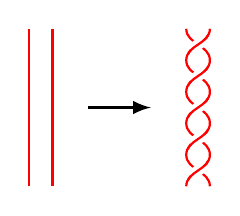
\begin{tikzpicture}[
                every to/.style={out=90,in=-90}
            ]
                \def\val{0.15}
                \begin{scope}[red, thick, xshift=-1cm]
                    \draw (-\val,-1) -- (-\val,1);
                    \draw (\val,-1) -- (\val,1);
                \end{scope}
                \draw[very thick,-latex] (-0.4,0) -- (0.4,0);
                \begin{knot}[
                    clip width=5,
                    clip radius=3pt,
                    every strand/.append style={red,thick},
                    xshift=1cm,
                    ignore endpoint intersections=false
                ]
                    \strand (-\val,-1) to (\val,-0.6) to (-\val,-0.2) to (\val,0.2) to (-\val,0.6) to (\val,1);
                    \strand (\val,-1) to (-\val,-0.6) to (\val,-0.2) to (-\val,0.2) to (\val,0.6) to (-\val,1);
                    \flipcrossings{2,4}
                \end{knot}
            \end{tikzpicture}
            \caption{A 5-move.}
            \label{fig:k-movesa}
        \end{subfigure}
        \begin{subfigure}[b]{0.2\linewidth}
            \centering
            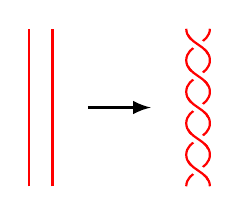
\begin{tikzpicture}[
                every to/.style={out=90,in=-90}
            ]
                \def\val{0.15}
                \begin{scope}[red, thick, xshift=-1cm]
                    \draw (-\val,-1) -- (-\val,1);
                    \draw (\val,-1) -- (\val,1);
                \end{scope}
                \draw[very thick,-latex] (-0.4,0) -- (0.4,0);
                \begin{knot}[
                    clip width=5,
                    clip radius=3pt,
                    every strand/.append style={red,thick},
                    xshift=1cm,
                    ignore endpoint intersections=false
                ]
                    \strand (\val,-1) to (-\val,-0.6) to (\val,-0.2) to (-\val,0.2) to (\val,0.6) to (-\val,1);
                    \strand (-\val,-1) to (\val,-0.6) to (-\val,-0.2) to (\val,0.2) to (-\val,0.6) to (\val,1);
                    \flipcrossings{2,4}
                \end{knot}
            \end{tikzpicture}
            \caption{A $-5$-move.}
            \label{fig:k-movesb}
        \end{subfigure}
        \caption{Examples of $k$-moves.}
        \label{fig:k-moves}
    \end{figure}
    \item \textbf{\emph{k}-equivalent}: Two knot or link projections that can be transformed into each other through a series of $k$-moves and $-k$-moves.
    \begin{itemize}
        \item Ambient isotropies are allowed between $k$-moves.
    \end{itemize}
    \item \emph{Exercise 3.8}: Show that the knots in Figure \ref{fig:ex3-8} are each three-equivalent to a trivial link.
    \begin{figure}[h!]
        \centering
        \begin{subfigure}[b]{0.3\linewidth}
            \centering
            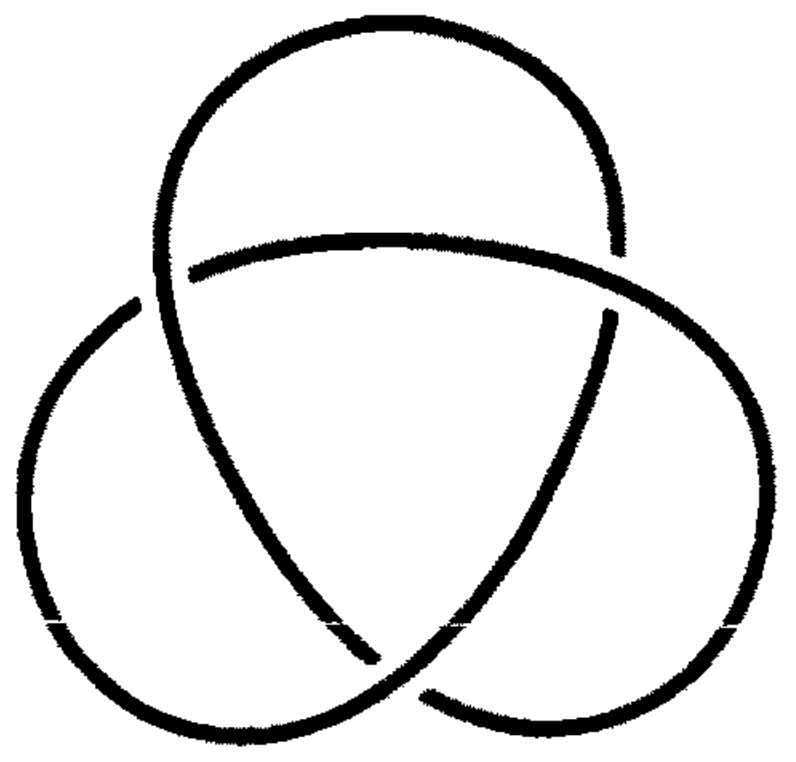
\includegraphics[width=0.5\linewidth]{Blender/ex3-8a.png}
            \caption{The knot $3_1$.}
            \label{fig:ex3-8a}
        \end{subfigure}
        \begin{subfigure}[b]{0.3\linewidth}
            \centering
            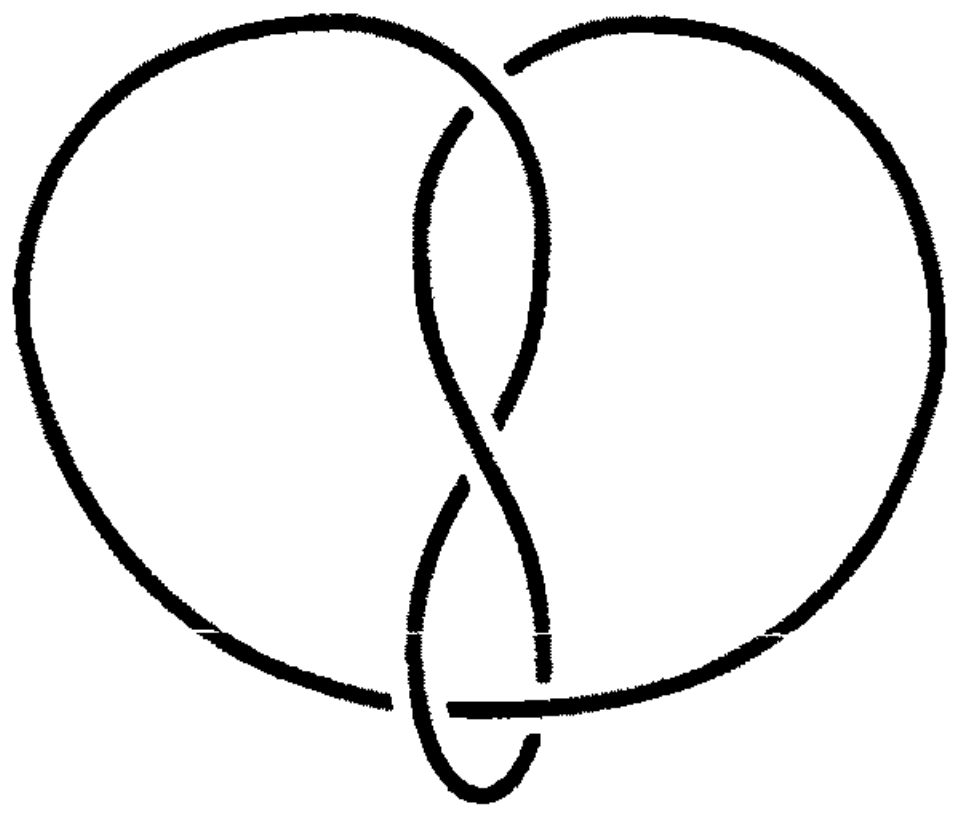
\includegraphics[width=0.55\linewidth]{Blender/ex3-8b.png}
            \caption{The knot $4_1$.}
            \label{fig:ex3-8b}
        \end{subfigure}
        \caption{Knots that are 3-equivalent to trivial links.}
        \label{fig:ex3-8}
    \end{figure}
    \begin{figure}[h!]
        \centering
        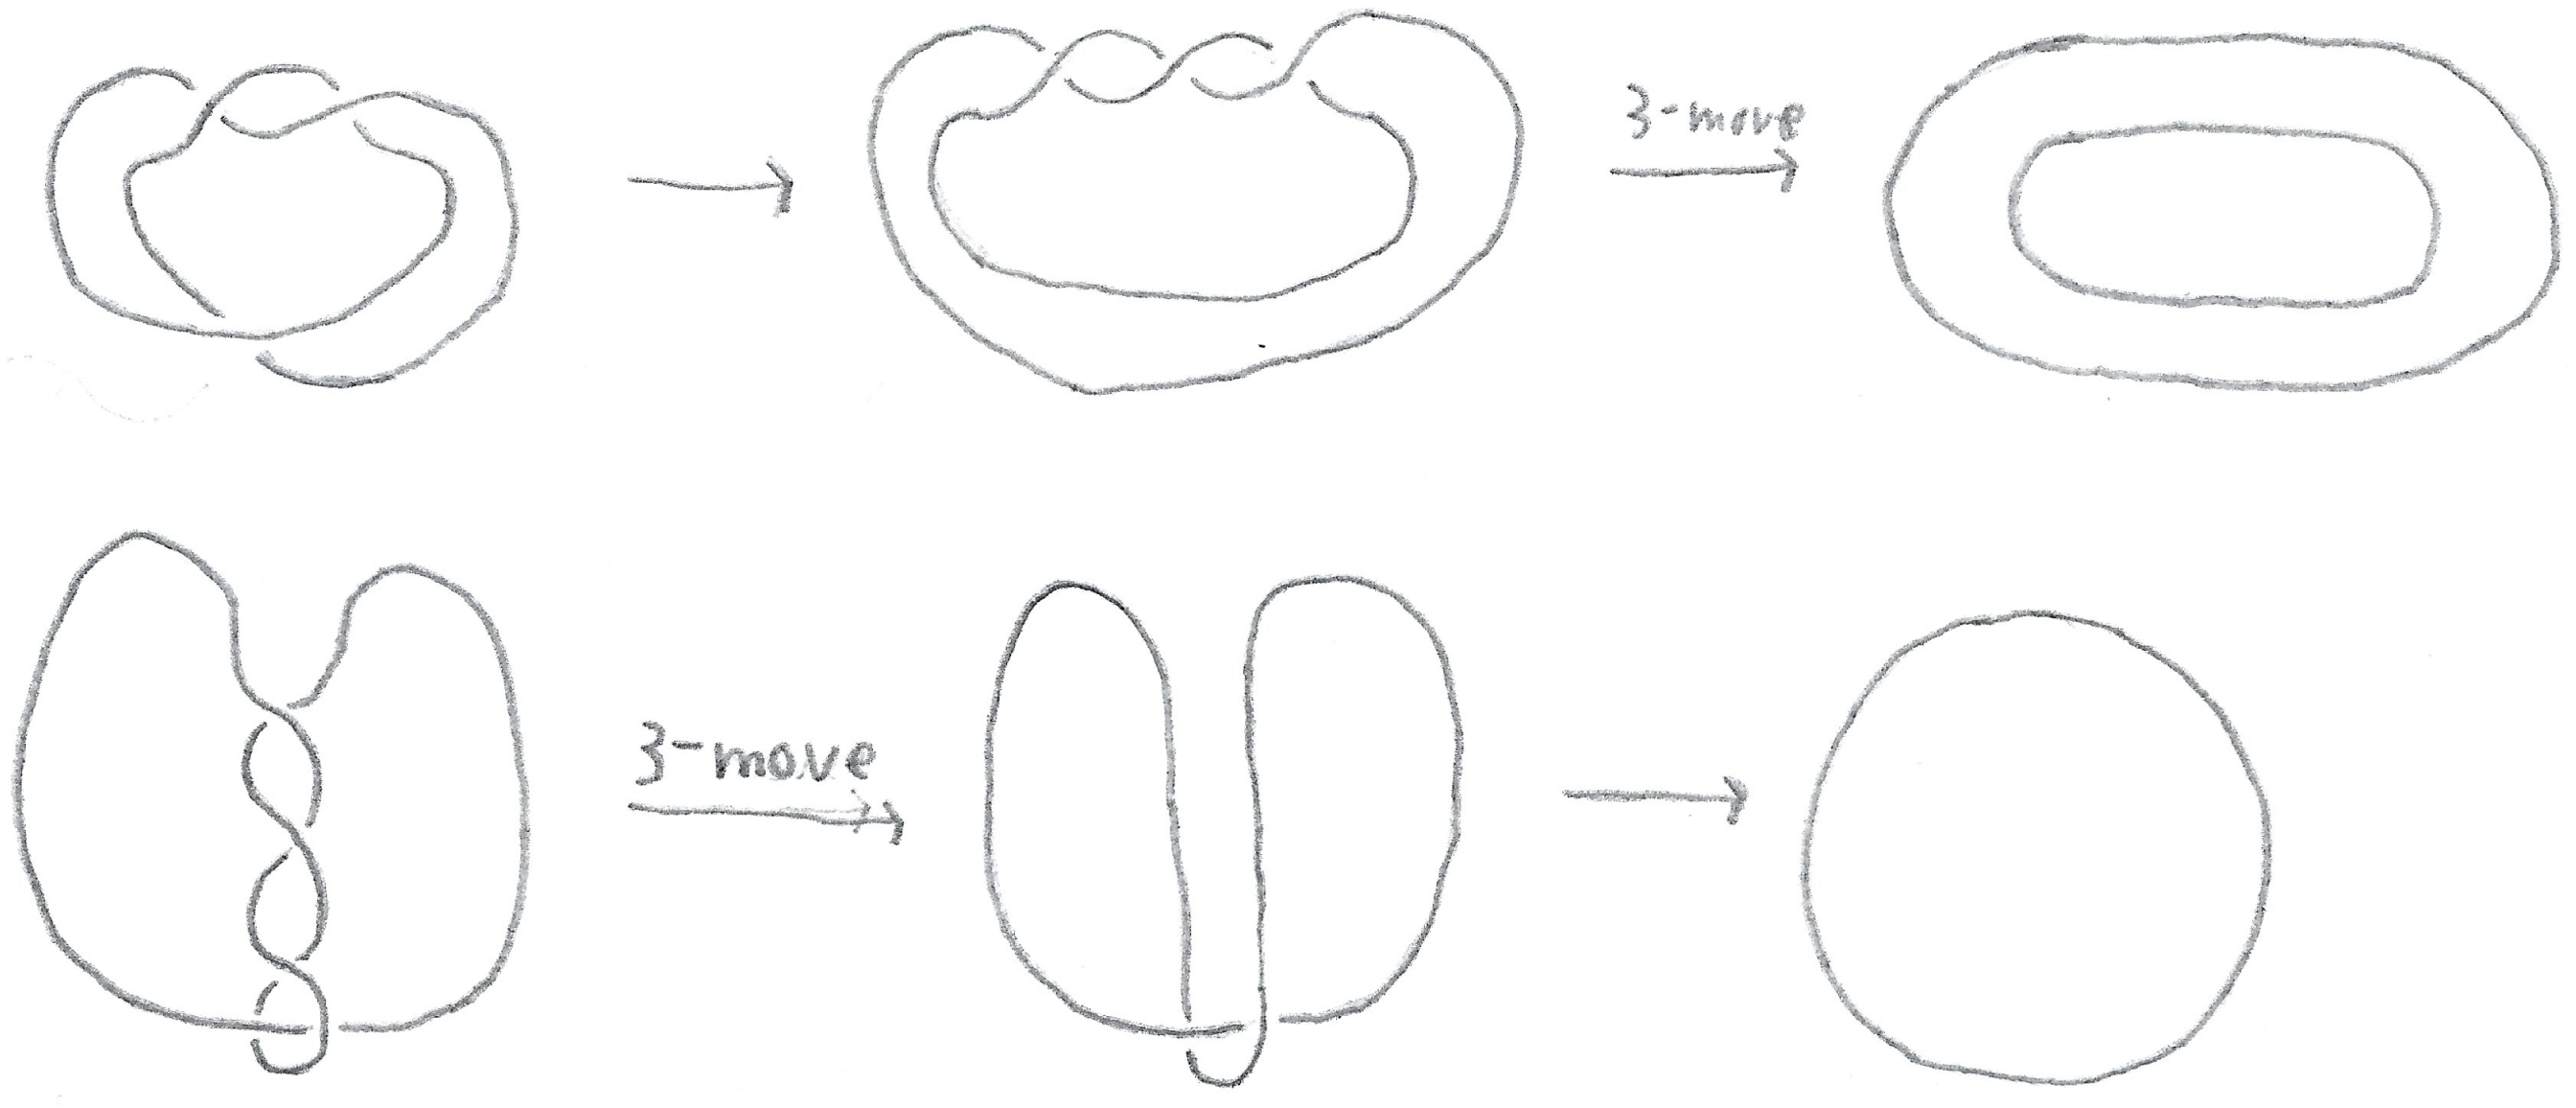
\includegraphics[width=0.7\linewidth]{Blender/ex3-8-2.png}
        \caption{Solution to \emph{Exercise 3.8}.}
        \label{fig:ex3-8-2}
    \end{figure}
\end{itemize}


\subsection{Bridge Number}
\begin{itemize}
    \item Think of knots as \dq{cutting through the projection plane, rather than lying in it}{64}
    \begin{itemize}
        \item Every overstrand is entirely above and every understrand is entirely beneath. The points where the strand shifts from over to under are known as \textbf{vertices}.
    \end{itemize}
    \item \textbf{Bridge number}: The least number of unknotted arcs lying above the plane in any projection of the knot. \emph{Also known as} $\mathbf{b(K)}$
    \begin{itemize}
        \item The number of maximal overpasses in in the projection.
    \end{itemize}
    \item \textbf{Overpass}: \dq{A subarc of the knot that goes over at least one crossing but never goes under a crossing}{64}
    \item \textbf{Maximal overpass}: \dq{An overpass that could not be made any longer}{65}
    \begin{figure}[h!]
        \centering
        \begin{subfigure}[b]{0.4\linewidth}
            \centering
            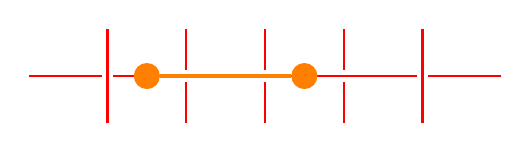
\begin{tikzpicture}
                \def\val{0.6}
                \begin{knot}[
                    clip width=5,
                    every strand/.append style={red,thick}
                ]
                    \strand (0,0) to (6,0);
                    \strand (1,-\val) to (1,\val);
                    \strand (2,-\val) to (2,\val);
                    \strand (3,-\val) to (3,\val);
                    \strand (4,-\val) to (4,\val);
                    \strand (5,-\val) to (5,\val);
                    \flipcrossings{1,5}
                \end{knot}
                \node [circle,fill=orange] (a) at (1.5,0) {};
                \node [circle,fill=orange] (b) at (3.5,0) {}
                    edge [ultra thick,orange] (a)
                ;
            \end{tikzpicture}
            \caption{An overpass.}
            \label{fig:overpassa}
        \end{subfigure}
        \begin{subfigure}[b]{0.4\linewidth}
            \centering
            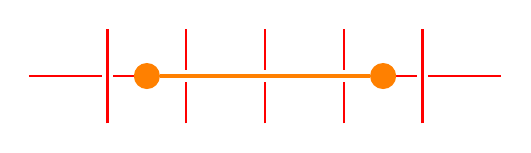
\begin{tikzpicture}
                \def\val{0.6}
                \begin{knot}[
                    clip width=5,
                    every strand/.append style={red,thick}
                ]
                    \strand (0,0) to (6,0);
                    \strand (1,-\val) to (1,\val);
                    \strand (2,-\val) to (2,\val);
                    \strand (3,-\val) to (3,\val);
                    \strand (4,-\val) to (4,\val);
                    \strand (5,-\val) to (5,\val);
                    \flipcrossings{1,5}
                \end{knot}
                \node [circle,fill=orange] (a) at (1.5,0) {};
                \node [circle,fill=orange] (b) at (4.5,0) {}
                    edge [ultra thick,orange] (a)
                ;
            \end{tikzpicture}
            \caption{A maximal overpass.}
            \label{fig:overpassb}
        \end{subfigure}
        \caption{Overpasses.}
        \label{fig:overpass}
    \end{figure}
    \item \emph{Exercise 3.10}: Show that if a knot has bridge number 1, it must be the unknot.
    \begin{itemize}
        \item If a knot has bridge number 1, $\exists$ a projection of the knot such that there is only one arc above the projection plane and 1 arc below the projection plane.
        \item This projection, viewed from above, will look like any isotropy of the knot. However, viewed from the side, there will be 0 crossings --- therefore, it is the unknot.
    \end{itemize}
    \item \emph{Exercise 3.11}: Show that the knot $5_2$ has bridge number 2$^[$\footnote{Idea for a paper: On reducing bridge number. Discuss manipulating a projection to its Dowker redraw to create the "killzone" and then using "killzone moves" to make the projection nonalternating.}$^]$.
    \begin{itemize}
        \item Since $5_2$ is distinct from the unknot, $b(K)\neq 1$.
        \item Therefore, the next possibility to check is 2. Then, a projection of $5_2$ with bridge number 2 $\Rightarrow b(k)=2$.
        \begin{figure}[h!]
            \centering
            \begin{subfigure}[b]{0.2\linewidth}
                \centering
                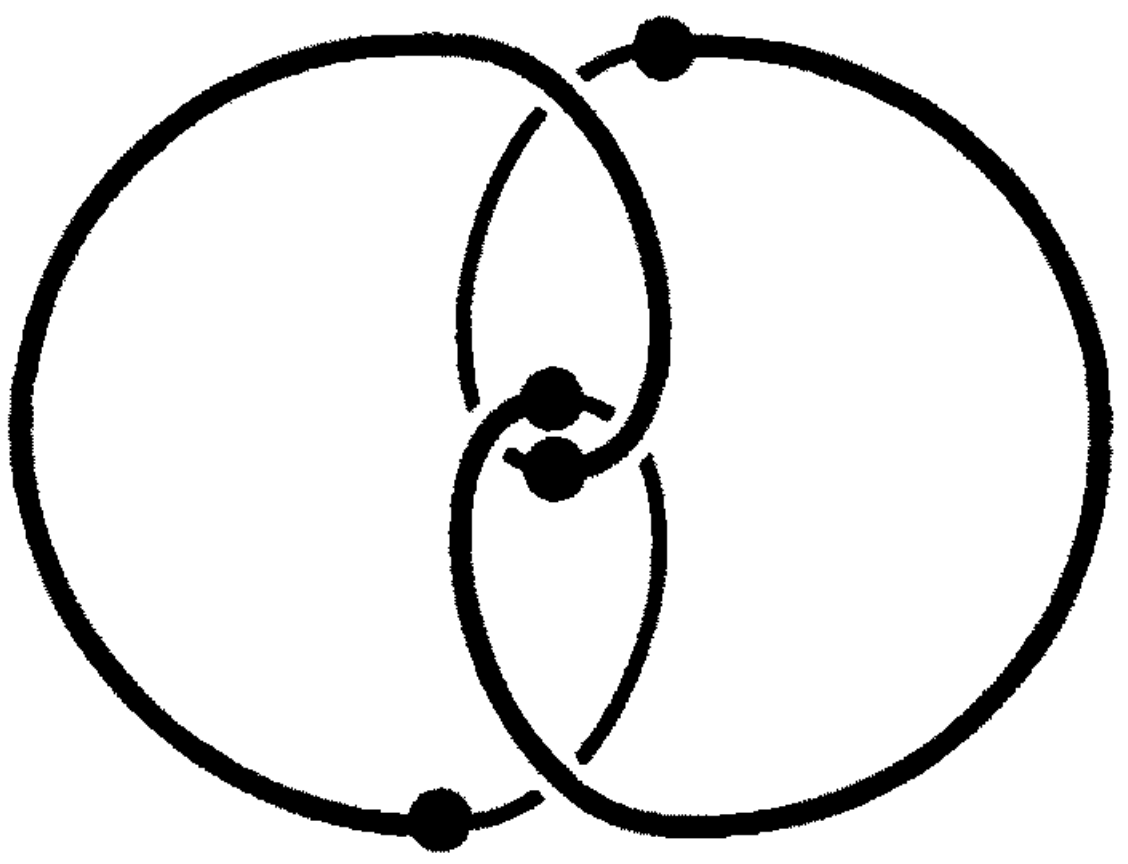
\includegraphics[width=0.8\linewidth]{Blender/ex3-11a.png}
                \caption{$3_1$ with $b(K)=2$.}
                \label{fig:ex3-11a}
            \end{subfigure}
            \begin{subfigure}[b]{0.2\linewidth}
                \centering
                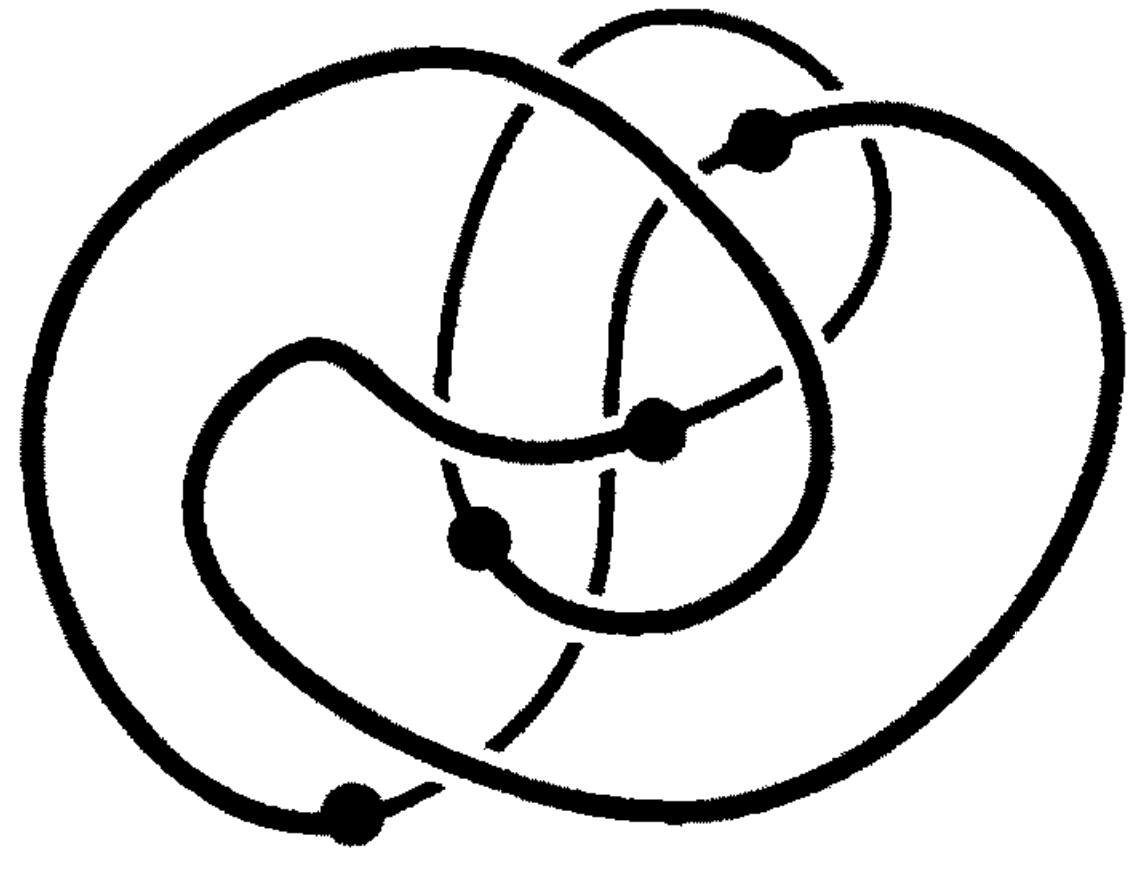
\includegraphics[width=0.8\linewidth]{Blender/ex3-11b.png}
                \caption{$4_1$ with $b(K)=2$.}
                \label{fig:ex3-11b}
            \end{subfigure}
            \caption{Reducing bridge number between projections.}
            \label{fig:ex3-11}
        \end{figure}
        \item Before tackling this problem, though, let's look at some simpler examples.
        \begin{itemize}
            \item From these, we notice that there are tangling moves which can reduce or increase the bridge number by $\pm 1$.
            \item Furthermore, long overstrands call to mind a Dowker reconstruction (Figure \ref{fig:reconstruction}).
        \end{itemize}
        \item Find the Dowker notation of $5_2$.
    \end{itemize}
\end{itemize}




\end{document}